
\documentclass[11pt,a4paper]{article}
\usepackage[margin=1in]{geometry}
\usepackage{graphicx}
\usepackage{grffile}
\usepackage{float}
\usepackage{booktabs}
\usepackage{longtable}
\usepackage{array}
\usepackage{multirow}
\usepackage{caption}
\usepackage{subcaption}
\usepackage{xcolor}
\usepackage{amsmath}
\usepackage{hyperref}
\usepackage{cleveref}
\usepackage{listings}
\usepackage{enumitem}
\usepackage{placeins}
\usepackage{pdflscape}
\usepackage{adjustbox}
\usepackage[numbers,sort&compress]{natbib}

\hypersetup{colorlinks=true, linkcolor=blue!55!black, citecolor=blue!55!black, urlcolor=blue!55!black}
\lstset{basicstyle=\ttfamily\scriptsize, breaklines=true, frame=single, columns=fullflexible, keepspaces=true, showstringspaces=false}
\captionsetup{font=small, labelfont=bf}
\setlist[itemize]{leftmargin=1.3em}
\setlength{\parskip}{0.35em}
\setlength{\parindent}{0pt}

\newif\ifincludeallresultgallery
\includeallresultgalleryfalse
% For a quick Overleaf preview, change the previous line to: \includeallresultgalleryfalse

\title{\textbf{Image Segmentation Using Adaptive Color--Spatial--Texture Feature Spaces}\\[0.3em]
\large Advanced Digital Image Processing (CSE 6243), Assignment 02}
\author{Student Name: \textbf{Your Name} \\ Roll No.: \textbf{Your Roll No.} \\ Department of Computer Science and Engineering, KUET}
\date{January Semester 2026}

\begin{document}
\maketitle
\begin{abstract}
This project implements unsupervised image segmentation using multiple feature-space representations built from color, normalized spatial location, and texture responses. The system prepares manual ground-truth masks and contours from LabelMe-style polygon annotations, generates segmentation outputs using MiniBatch K-means and Mean Shift clustering, applies connected-component post-processing, and evaluates each result against ground truth after label matching. The submitted material contains \textbf{478 post-processed segmentation cases} across ten images, full program files, self and peer ground-truth images, annotation files, qualitative output images, and CSV files containing Precision, Recall, IoU, Boundary F1-score, and normalized confusion matrix values. A peer-ground-truth test is also included using the selected best prediction for each image.
\end{abstract}

\tableofcontents
\listoffigures
\listoftables
\clearpage


\section{Introduction}
Image segmentation partitions an image into visually meaningful regions. In this assignment the goal is not only to produce a segmented image, but to design and test feature spaces that make clustering easier. A single RGB pixel value is usually insufficient because similar objects may have different illumination, and different objects may share similar colors. The core idea of this project is therefore to describe every pixel with a richer vector containing some or all of the following components:
\begin{itemize}
    \item normalized spatial coordinates $(x,y)$, which encourage spatially coherent regions;
    \item color channels from RGB, HSV, and Lab spaces, which describe appearance from complementary viewpoints;
    \item texture responses from filter banks or statistical texture descriptors, which help separate surfaces that are similar in color but different in local pattern;
    \item dimension reduction and sampling strategies so that Mean Shift remains practical for high-dimensional feature spaces.
\end{itemize}

The project evaluates these feature spaces with two unsupervised clustering algorithms: MiniBatch K-means and Mean Shift. K-means gives a fast baseline with a fixed number of regions, while Mean Shift estimates modes in feature space and can adapt the number of clusters to the data distribution \citep{macqueen1967,llyod1982,comaniciu2002}. The segmentation masks are then post-processed and compared with the manually prepared ground truth using label matching, normalized confusion matrices, Precision, Recall, Intersection-over-Union (IoU), and Boundary F1-score.

\textbf{Main contribution.} The implemented method is an adaptive color--spatial--texture segmentation pipeline. Instead of using one fixed feature vector for all images, the project tests separate features and combinations, then uses the most suitable texture family and computational mode according to image scale and visual structure. This makes the project stronger than a direct ``RGB + K-means'' implementation because it systematically studies how each feature source affects segmentation quality.


\section{Dataset, Annotation, and Ground Truth Preparation}
\subsection{Assignment requirements covered}
The submitted package follows the requested deliverable structure. It contains manual ground-truth masks and contours, machine generated output images, peer ground-truth images, annotation JSON files, Python program files, and CSV numerical results. The quantitative CSV files are stored under \texttt{numerical\_results/}, while the raw output images are stored under \texttt{outputs/}.

\begin{table}[H]
\centering
\caption{Project material summary.}
\begin{tabular}{@{}lr@{}}
\toprule
Item & Count / description \\
\midrule
Input images with self GT & 10 images \\
Post-processed segmentation cases & 478 cases \\
Unique feature-space labels in outputs & 45 feature-set names \\
Peer GT images used for additional evaluation & 10 images \\
Program files & \texttt{main\_3\_final.py}, \texttt{datasetCreation.py}, \texttt{evaluate\_2.py} \\
Numerical result format & CSV files for per-image, per-class, confusion-matrix, and summary metrics \\
\bottomrule
\end{tabular}
\label{tab:material-summary}
\end{table}

\subsection{Manual annotation format}
The ground truth was prepared with polygon annotations in a LabelMe-style JSON file. Each annotated object or region is stored as a polygon with a semantic label and a list of $(x,y)$ points. The file is then rasterized into three useful ground-truth products: a filled mask, a contour image, and a contour overlay on the original image. This representation is convenient because the JSON remains editable, while the raster masks are directly usable for pixel-level evaluation.

\begin{figure}[H]
\centering
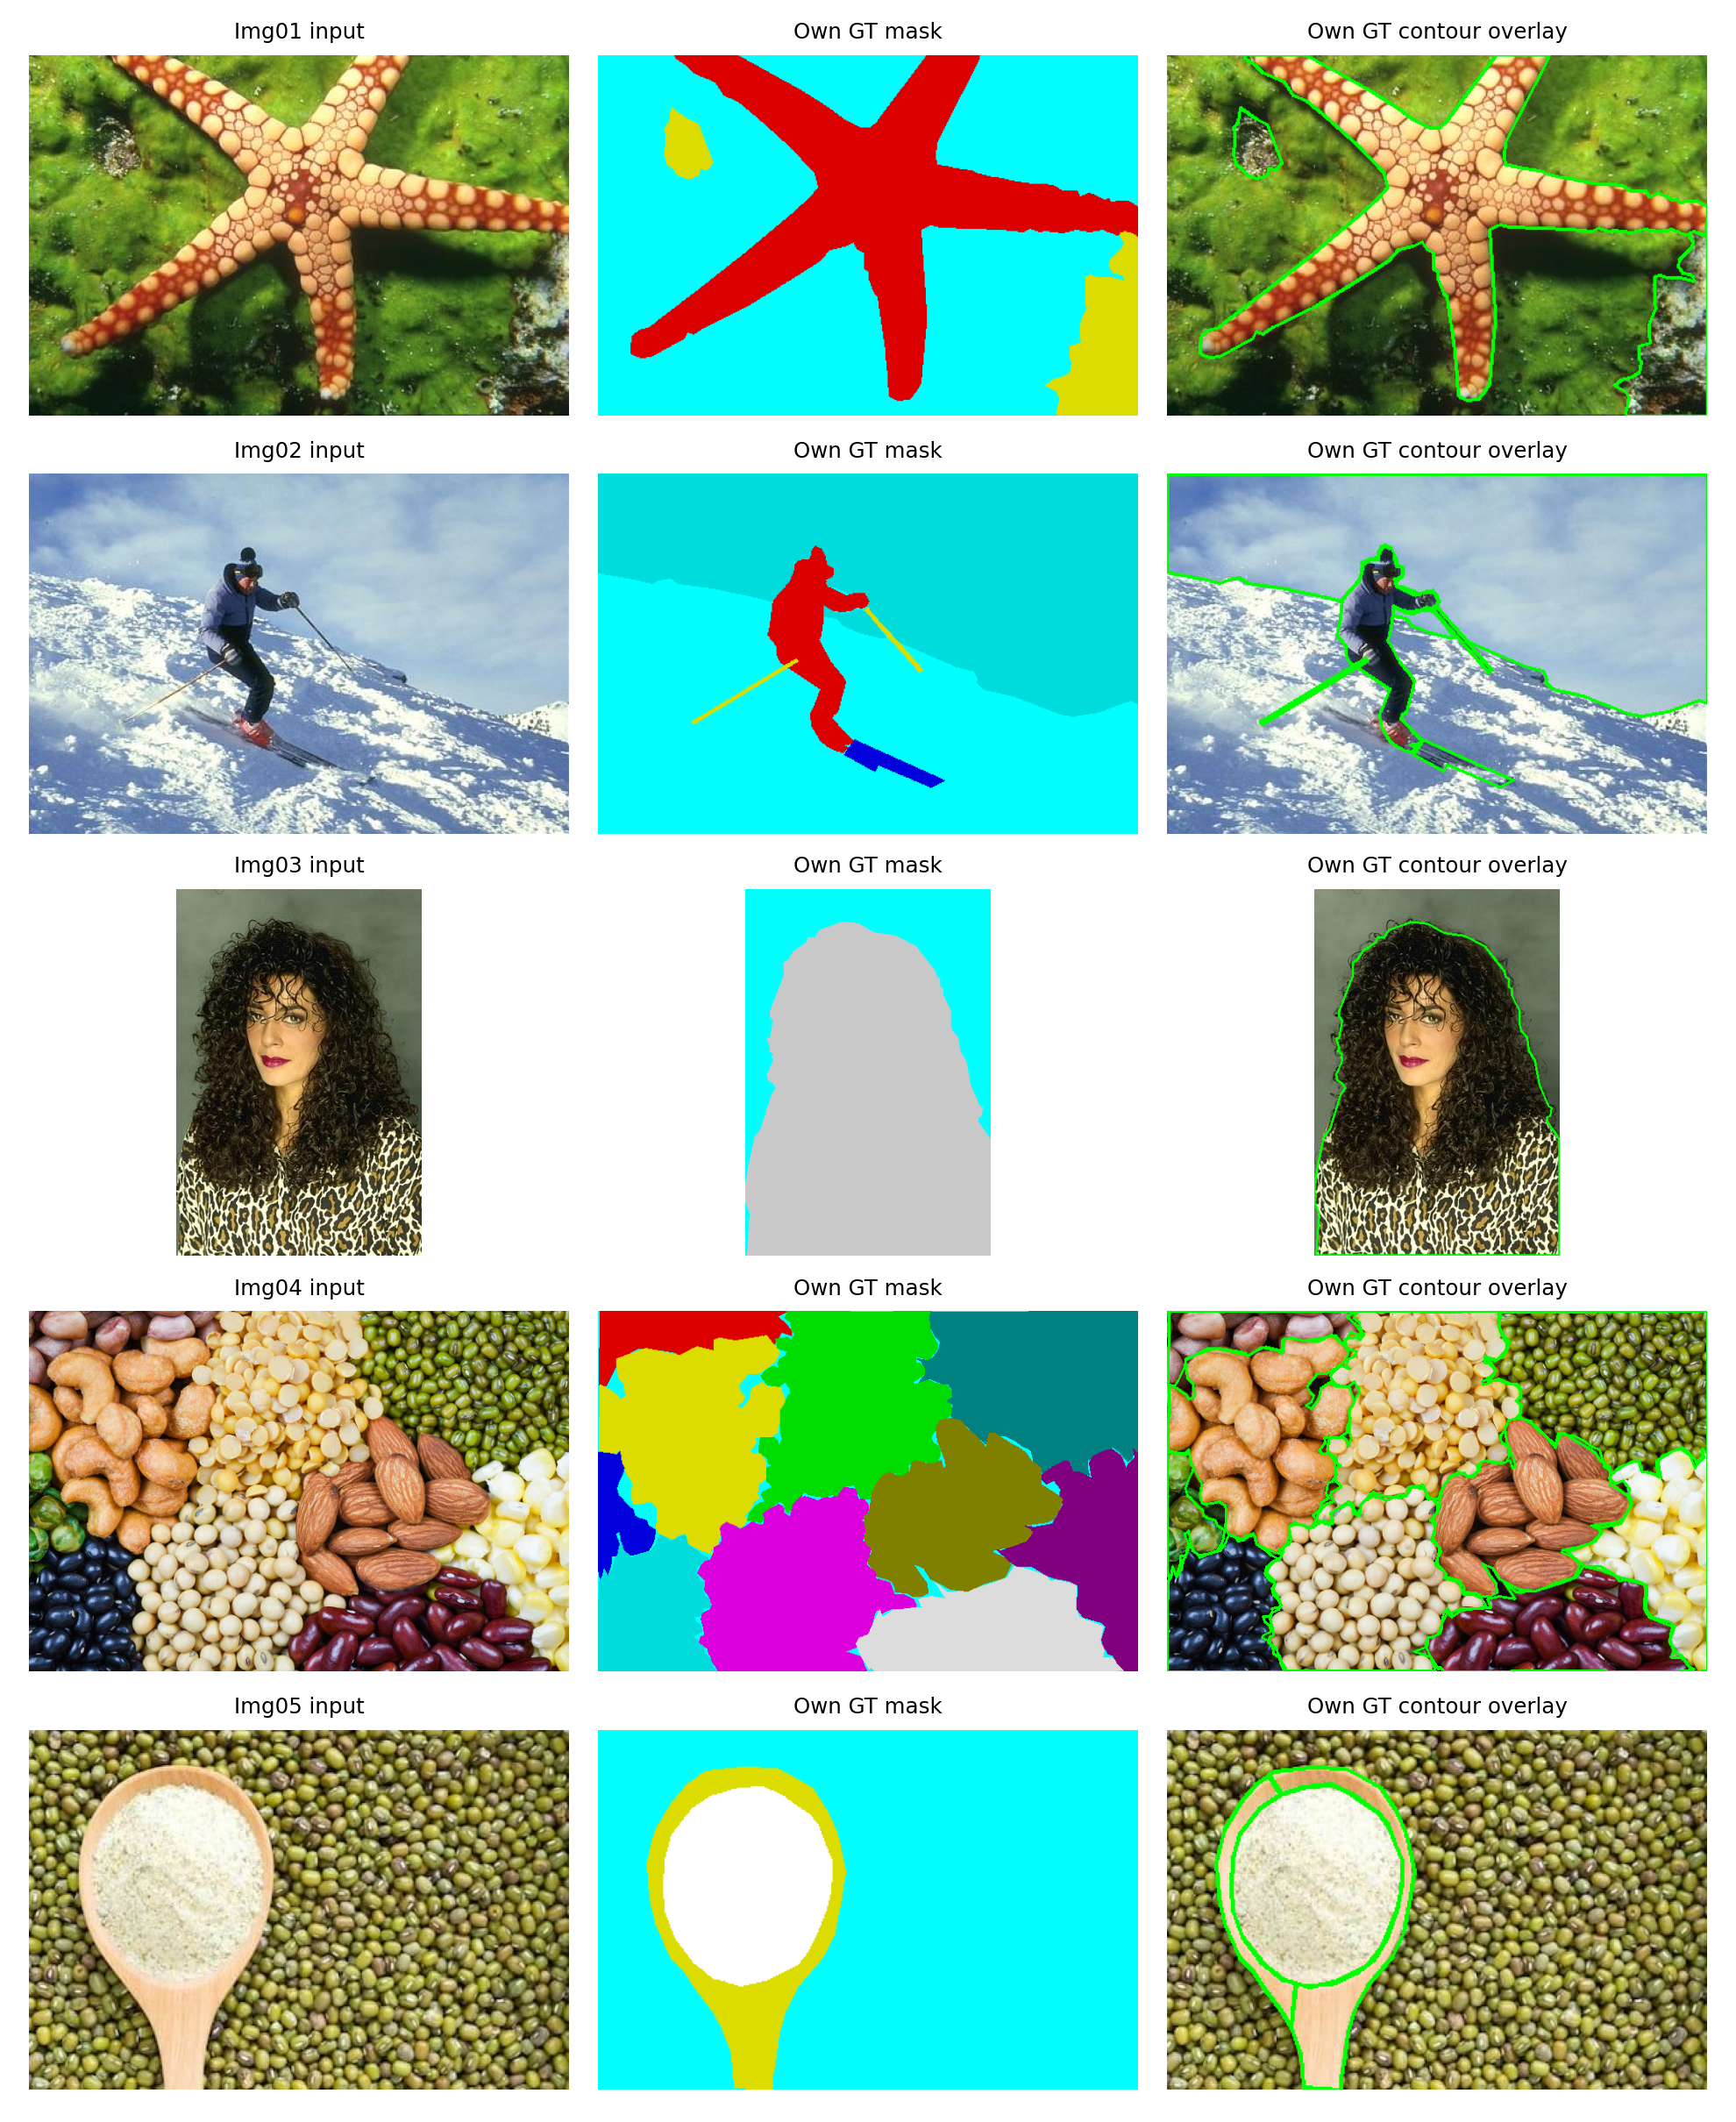
\includegraphics[width=0.88\textwidth,height=0.42\textheight,keepaspectratio]{figures/grids/own_gt_gallery_part1.png}
\caption{Self-created ground-truth examples for Images 01--05. Each row shows the input image, the filled GT mask, and the contour overlay.}
\label{fig:own-gt-gallery-a}
\end{figure}
\begin{figure}[H]
\centering
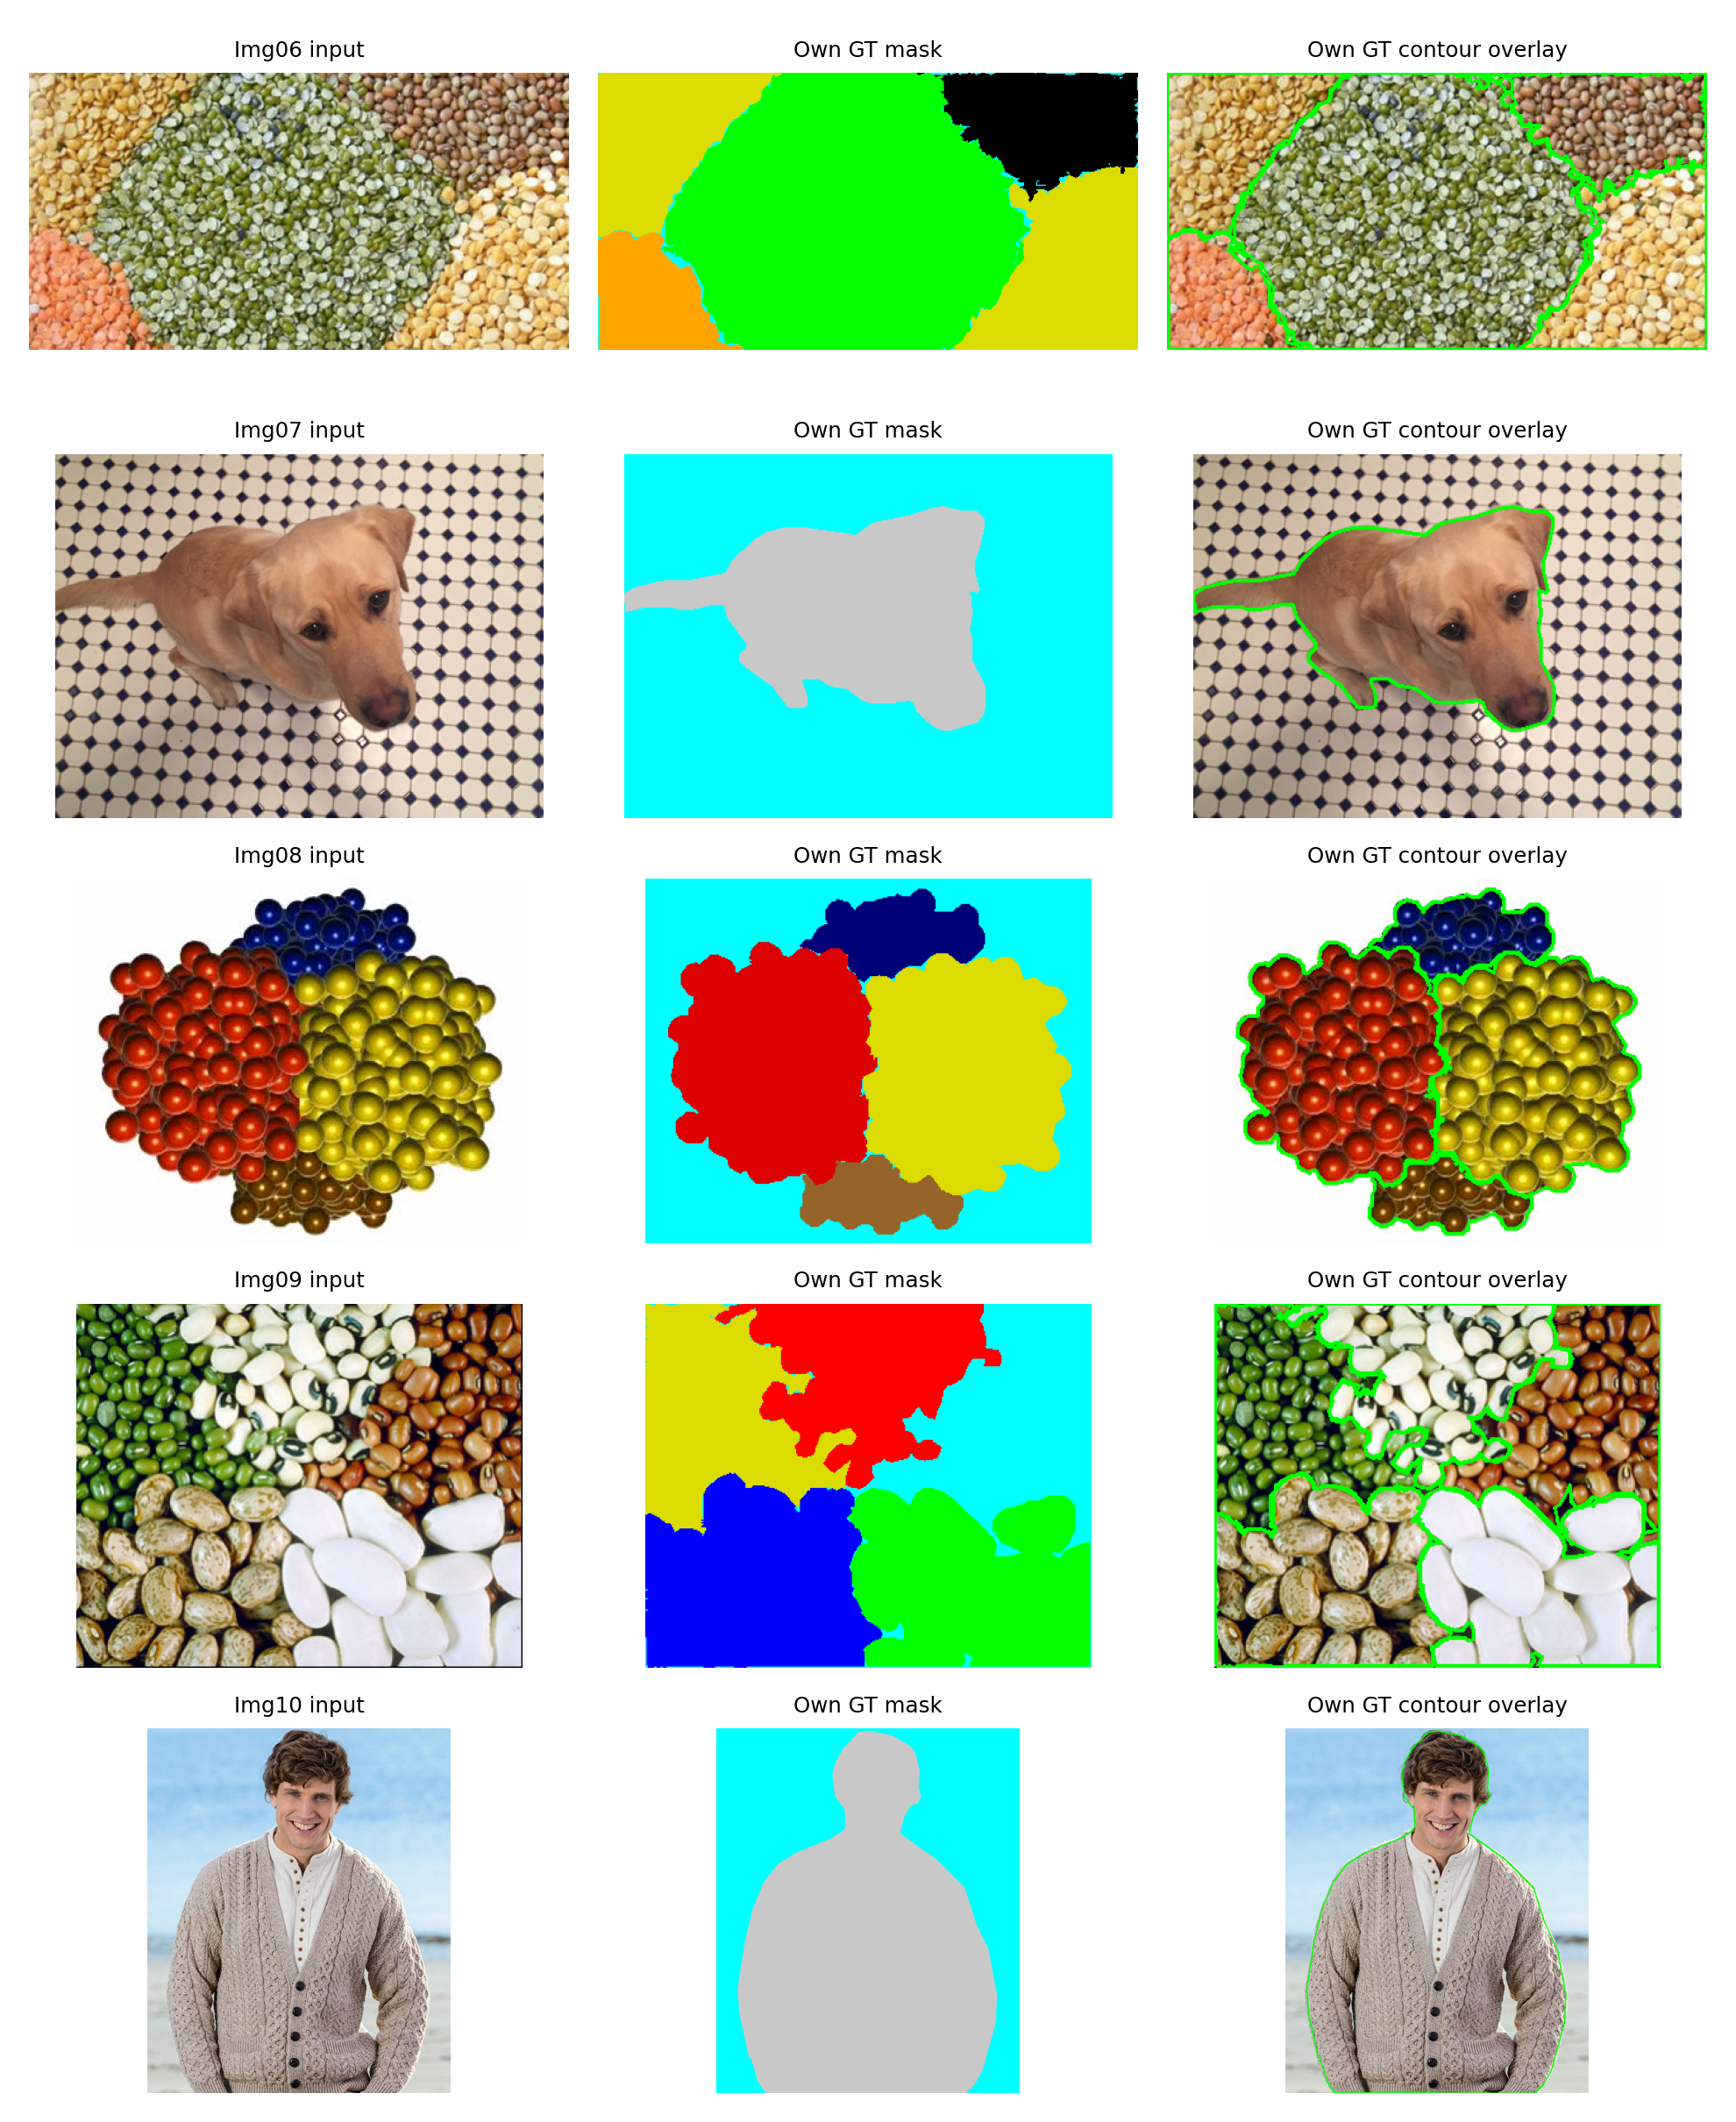
\includegraphics[width=0.88\textwidth,height=0.42\textheight,keepaspectratio]{figures/grids/own_gt_gallery_part2.png}
\caption{Self-created ground-truth examples for Images 06--10. The complete GT folders are included in \texttt{outputs/GT Ehsanul Karim/} and editable JSON files are included in \texttt{annotations/self/}.}
\label{fig:own-gt-gallery-b}
\end{figure}

\subsection{Why masks, contours, and overlays are all stored}
The mask image is used for quantitative pixel-level evaluation. The contour image is used to visually inspect boundary quality and to blend self and peer annotations. The overlay image makes the annotation quality easy to check against the input image. Keeping all three forms prevents ambiguity: masks support metrics, contours support boundary inspection, and overlays support qualitative reporting.


\section{Proposed Methodology}
\subsection{Feature-space design}
For every pixel, the program builds a feature vector from one or more feature groups. Each feature channel is normalized before clustering so that one scale, such as spatial coordinate or Lab intensity, does not dominate the distance function. The tested feature groups are:
\begin{itemize}
    \item \textbf{XY:} normalized horizontal and vertical pixel positions;
    \item \textbf{RGB:} raw color channels in the standard red, green, and blue representation;
    \item \textbf{HSV:} hue, saturation, and value channels for illumination-aware color separation;
    \item \textbf{Lab:} perceptually motivated lightness and chromaticity channels;
    \item \textbf{Texture:} local texture responses using Gabor, Leung--Malik, or GLCM-style descriptors depending on the image group;
    \item \textbf{Combinations:} XY + color, XY + texture, color + texture, and XY + color + texture.
\end{itemize}

The idea is that color separates regions with different appearance, XY penalizes spatially scattered clusters, and texture separates regions with similar color but different surface pattern. This is especially useful for natural images where object boundaries are often defined by texture changes rather than color alone.

\subsection{Texture features}
Gabor filters are useful for orientation- and frequency-selective texture analysis. In this implementation a multi-scale, multi-orientation bank is applied to the grayscale image and the absolute filter responses are used as texture channels. For images where material-like texture is more important, a Leung--Malik-style bank of Gaussian derivatives and isotropic filters is used. For some images, GLCM-style texture outputs are included in the generated results, especially where co-occurrence statistics were more stable than direct filter responses.

\begin{figure}[H]
\centering
\begin{subfigure}{0.47\textwidth}
\centering
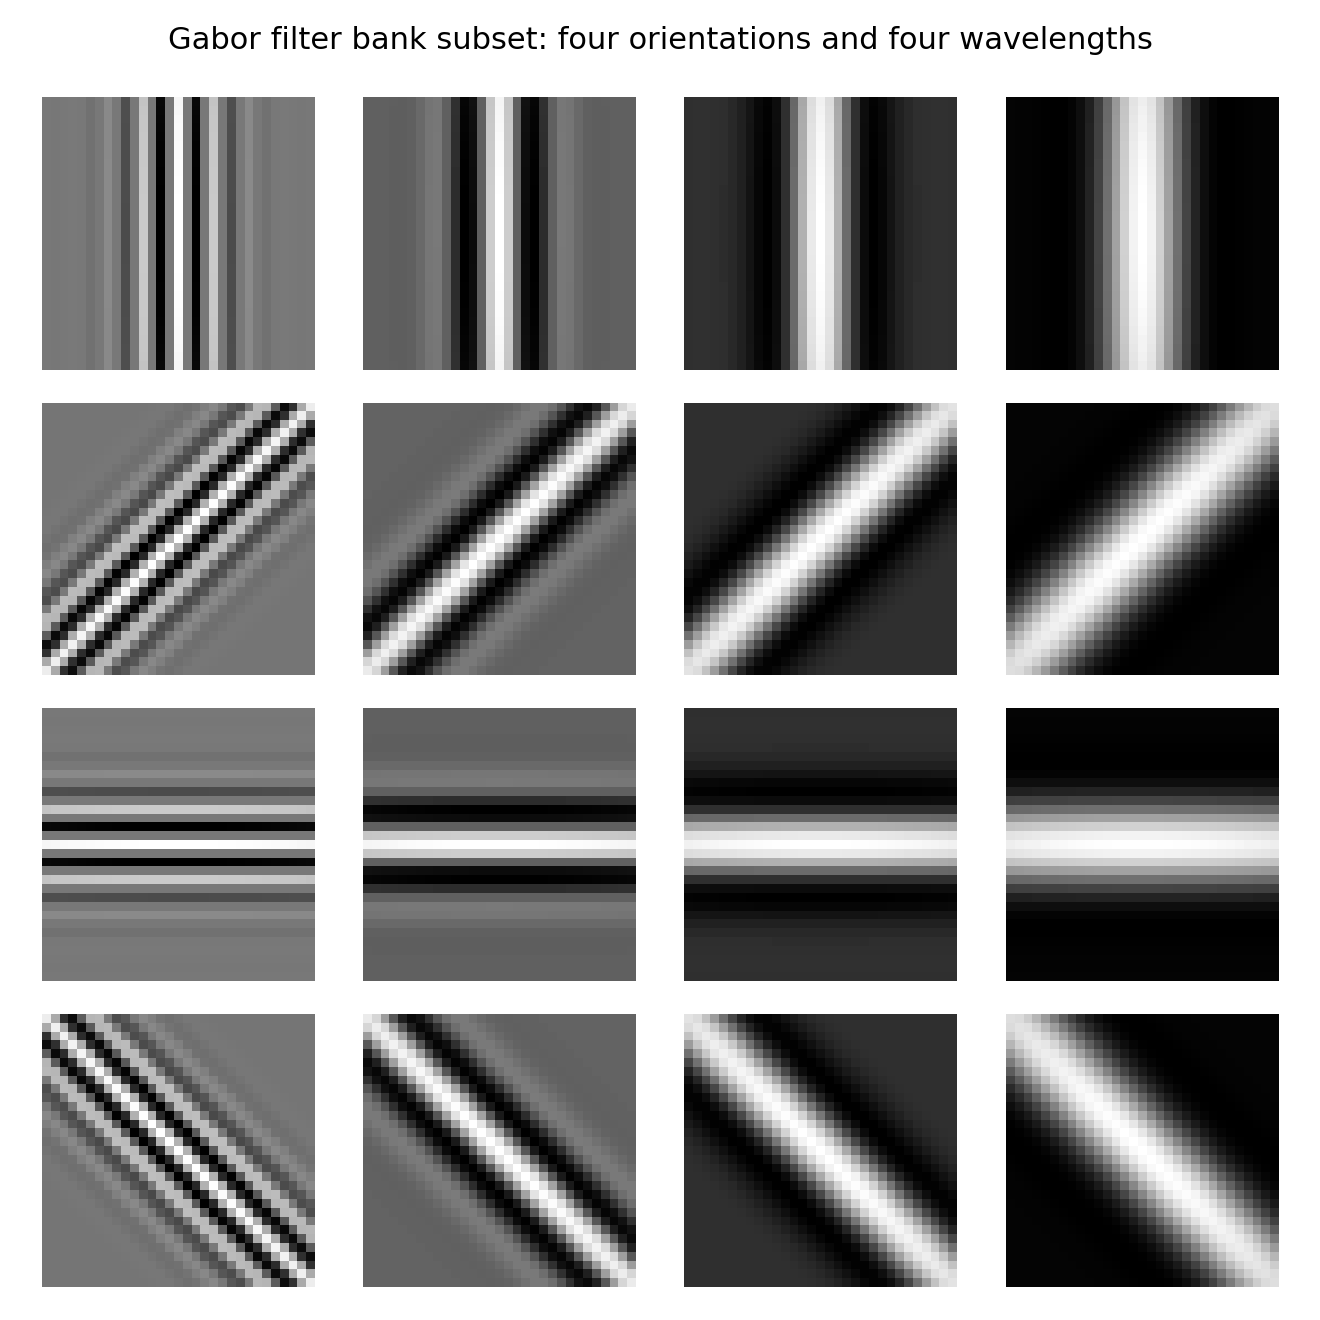
\includegraphics[width=\textwidth]{figures/method/gabor_filter_bank_subset.png}
\caption{Subset of the Gabor bank.}
\end{subfigure}\hfill
\begin{subfigure}{0.47\textwidth}
\centering
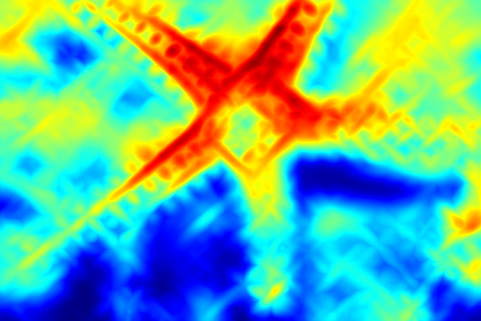
\includegraphics[width=\textwidth]{figures/method/gabor_activation_img01.png}
\caption{JET heat map of maximum Gabor response on Image 01.}
\end{subfigure}
\caption{Gabor filter visualization and response map. The heat map highlights pixels where at least one filter in the bank activates strongly.}
\label{fig:gabor-method}
\end{figure}

\begin{figure}[H]
\centering
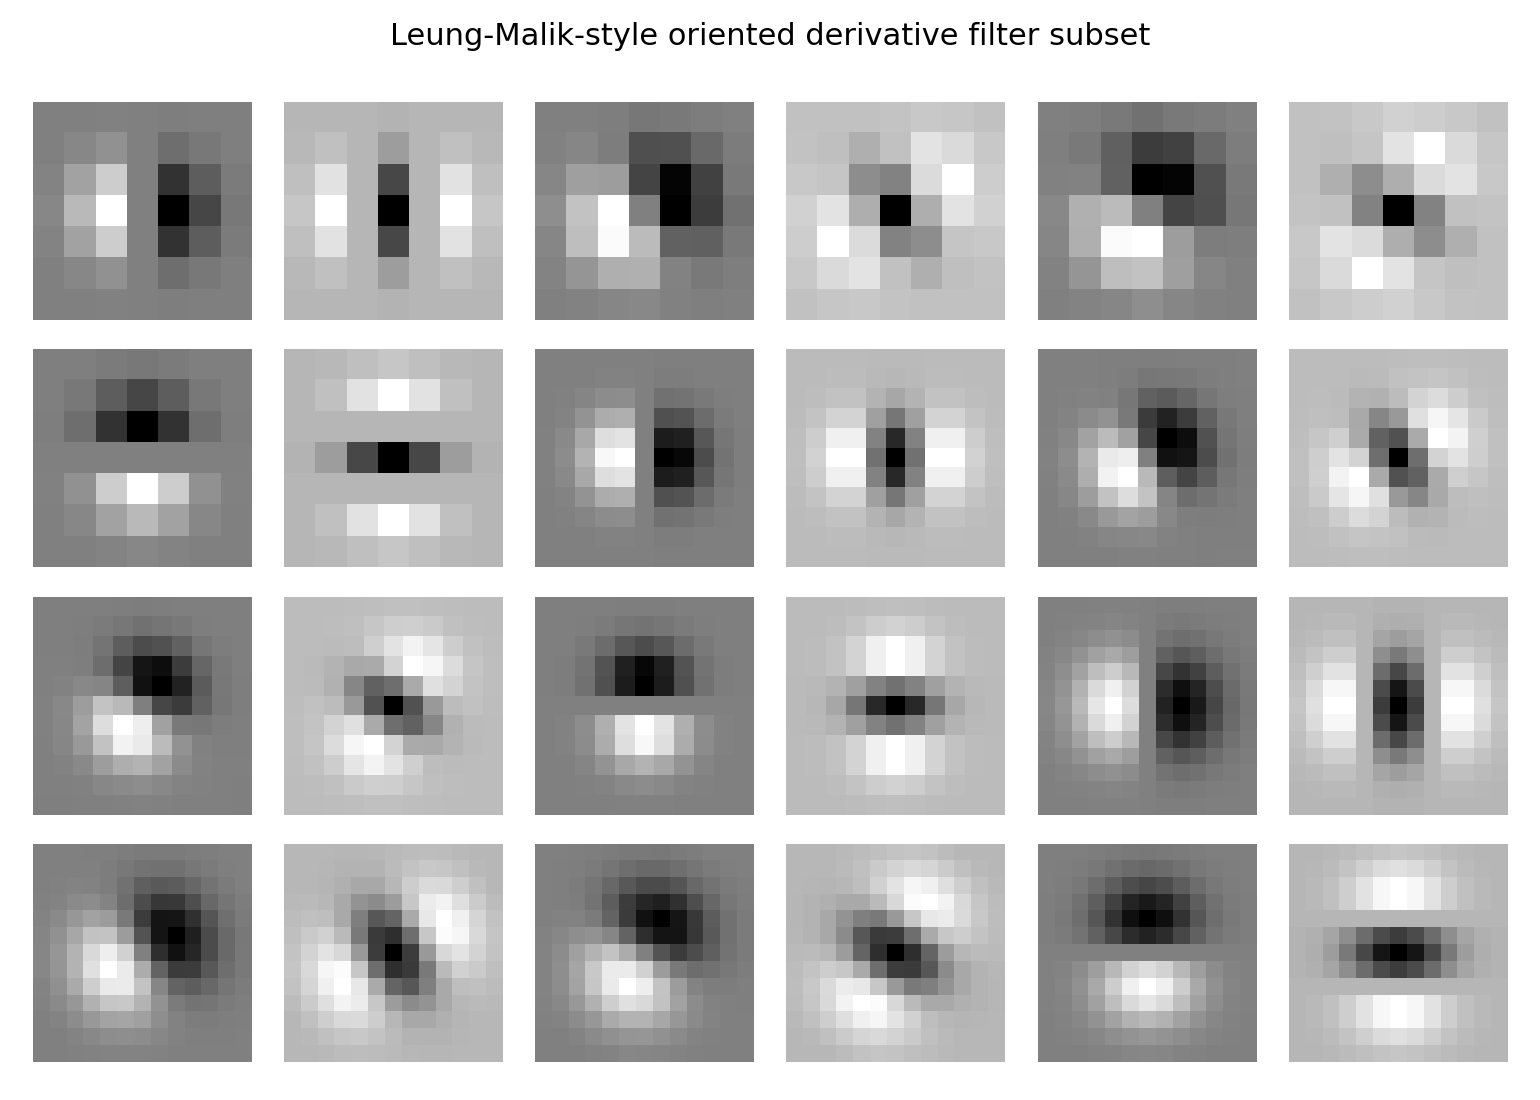
\includegraphics[width=0.72\textwidth]{figures/method/lm_filter_bank_subset.png}
\caption{Representative subset of the Leung--Malik-style oriented derivative filter bank used for texture representation.}
\label{fig:lm-method}
\end{figure}

\subsection{Clustering algorithms}
Two unsupervised clustering strategies are used.
\textbf{MiniBatch K-means} is used as the fast fixed-cluster baseline. It uses K-means++ initialization and mini-batches to reduce computation time. Most runs use $K=5$, while additional $K=4$ and $K=10$ outputs are stored for selected images to study under- and over-segmentation.

\textbf{Mean Shift} is used as an adaptive mode-seeking method. Two bandwidth values are tested in most output batches. Because Mean Shift becomes expensive in high-dimensional spaces, the implementation includes three practical modes: sampled Mean Shift, quarter-size Mean Shift, and half-size Mean Shift with PCA retaining 95\% variance. This directly follows the assignment note that resizing and PCA may be used to make Mean Shift feasible.

\subsection{Post-processing}
After clustering, small connected components are removed. Each small component is assigned to the most common surrounding label in a local dilation neighborhood. This step reduces isolated fragments and makes the segmentation more region-like without changing the main cluster structure. The report and CSVs use the post-processed masks, which are the final deliverable outputs.


\section{Implementation Details}
The project is implemented in Python using OpenCV, NumPy, scikit-learn, SciPy, Pillow, Pandas, and Matplotlib. The main program is menu-driven and saves every output to a predefined folder, so the results are reproducible and do not remain only as screen previews.

\begin{table}[H]
\centering
\caption{Main program components.}
\begin{tabular}{@{}p{0.28\textwidth}p{0.64\textwidth}@{}}
\toprule
File & Purpose \\
\midrule
\texttt{main\_3\_final.py} & Builds feature spaces, runs MiniBatch K-means and Mean Shift, saves raw and post-processed segmentation outputs. \\
\texttt{datasetCreation.py} & Converts annotation JSON polygons into mask, contour, and contour-overlay GT images. \\
\texttt{evaluate\_2.py} & Evaluates segmentation masks against GT using label matching, confusion matrices, Precision, Recall, IoU, and Boundary F1-score. \\
\texttt{fast\_eval\_minimal.py} & Helper script used in this package to regenerate compact CSV summaries quickly. \\
\texttt{evaluate\_peer\_selected.py} & Helper script used to evaluate selected best predictions against peer GT. \\
\bottomrule
\end{tabular}
\label{tab:program-components}
\end{table}

\subsection{Output folder convention}
The output folder is organized by image, feature space, and algorithm. For example, a typical result is stored as:
\begin{lstlisting}
outputs/Img01/xy_hsv/Half Resize PCA 95 Mean Shift/Post Processed Img01-meanshift-0.8.png
\end{lstlisting}
This path tells us the image ID, feature set, Mean Shift computation mode, and bandwidth parameter. K-means outputs are stored similarly under a \texttt{KMeans} subfolder.

\subsection{Evaluation protocol}
The machine-generated segmentation labels do not necessarily have the same numeric/color IDs as the GT labels, so label matching is required before measuring metrics. This package uses many-to-one label matching in the regenerated CSV summaries. That choice is suitable for segmentation because an algorithm may over-segment a single GT object into several pieces; those pieces should still be allowed to map to the same GT class for pixel-level scoring. The normalized confusion matrix is then computed after matching.

The per-class measures are:
\begin{align}
\mathrm{Precision} &= \frac{TP}{TP + FP}, &
\mathrm{Recall} &= \frac{TP}{TP + FN}, &
\mathrm{IoU} &= \frac{TP}{TP + FP + FN}.
\end{align}
Boundary F1-score is computed by extracting class boundaries and allowing a tolerance of 2 pixels. Macro scores are averaged over foreground classes, with background excluded from the macro average but still recorded in the per-class CSV files.


\section{Results and Analysis}
\subsection{Qualitative results}
\Cref{fig:best-qualitative-a,fig:best-qualitative-b} shows the best selected result for each image according to own-GT macro IoU. The full appendix includes the complete output gallery with all 478 post-processed result cases. In the main report, these selected examples show how the feature-space combinations behave across different images.

\begin{figure}[H]
\centering
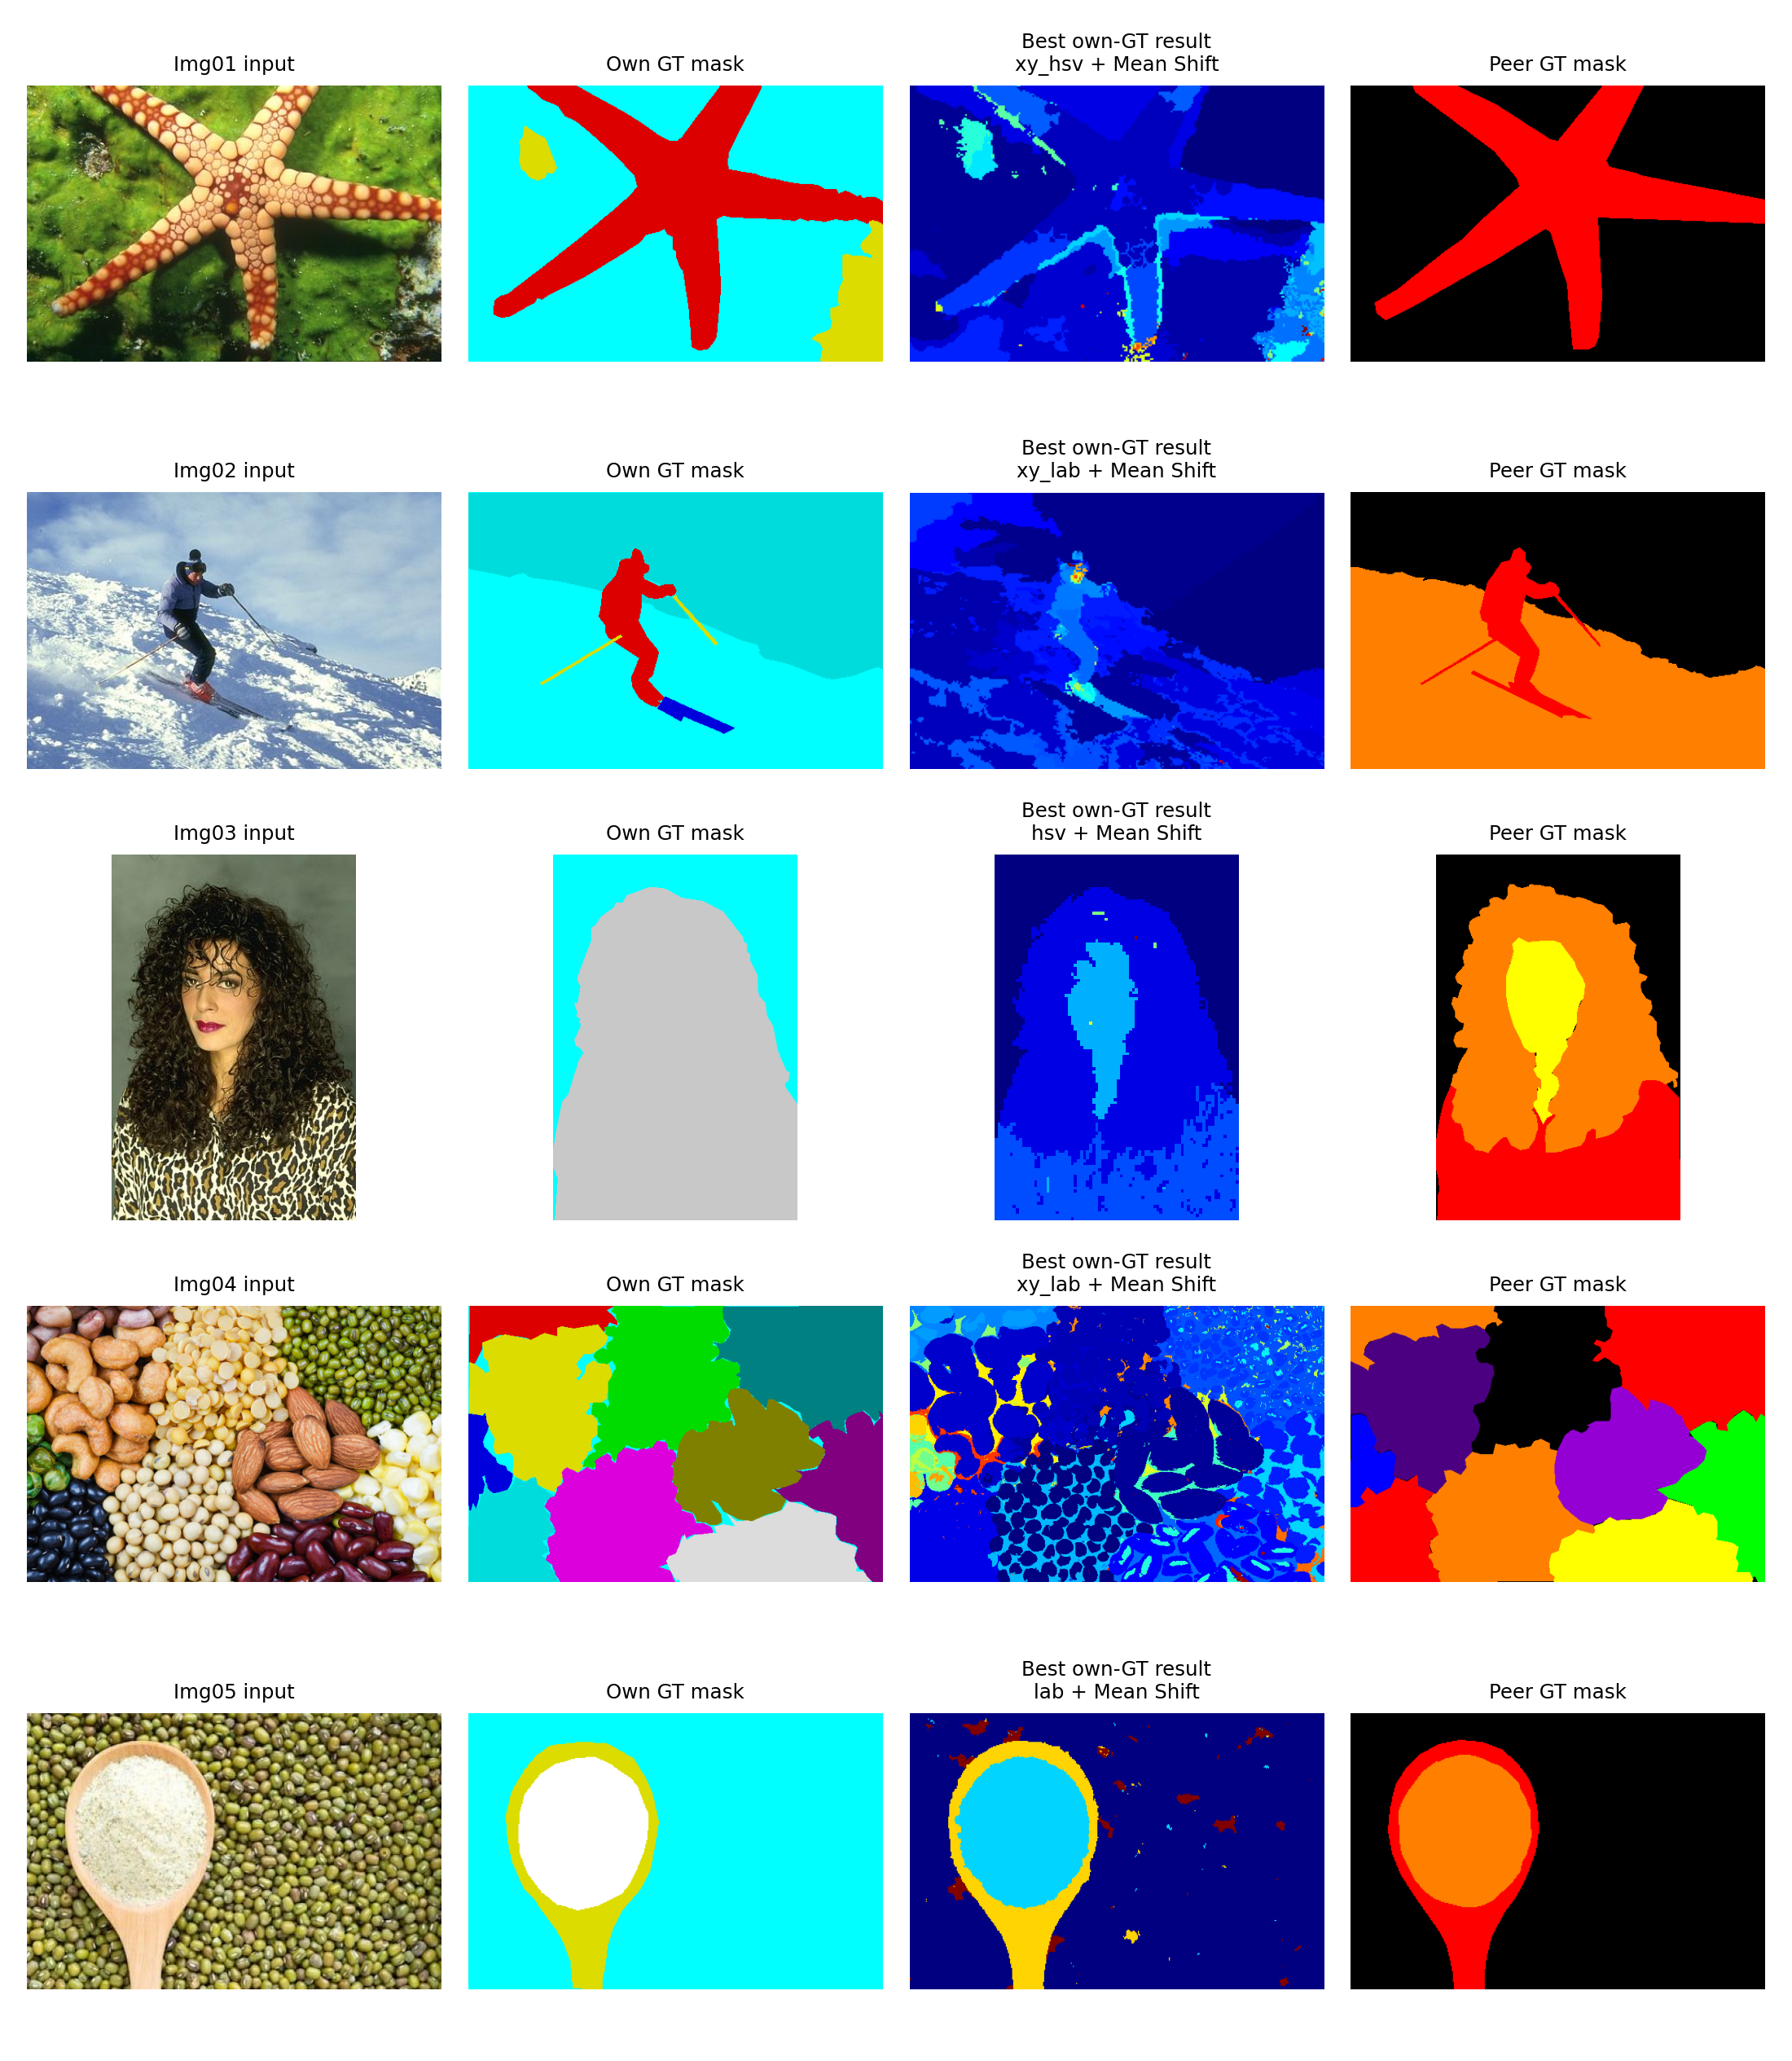
\includegraphics[width=0.95\textwidth,height=0.43\textheight,keepaspectratio]{figures/grids/best_qualitative_results_part1.png}
\caption{Best qualitative segmentation examples for Images 01--05, selected per image using own-GT macro IoU. Each row shows the input, own GT mask, selected machine output, and peer GT mask.}
\label{fig:best-qualitative-a}
\end{figure}
\begin{figure}[H]
\centering
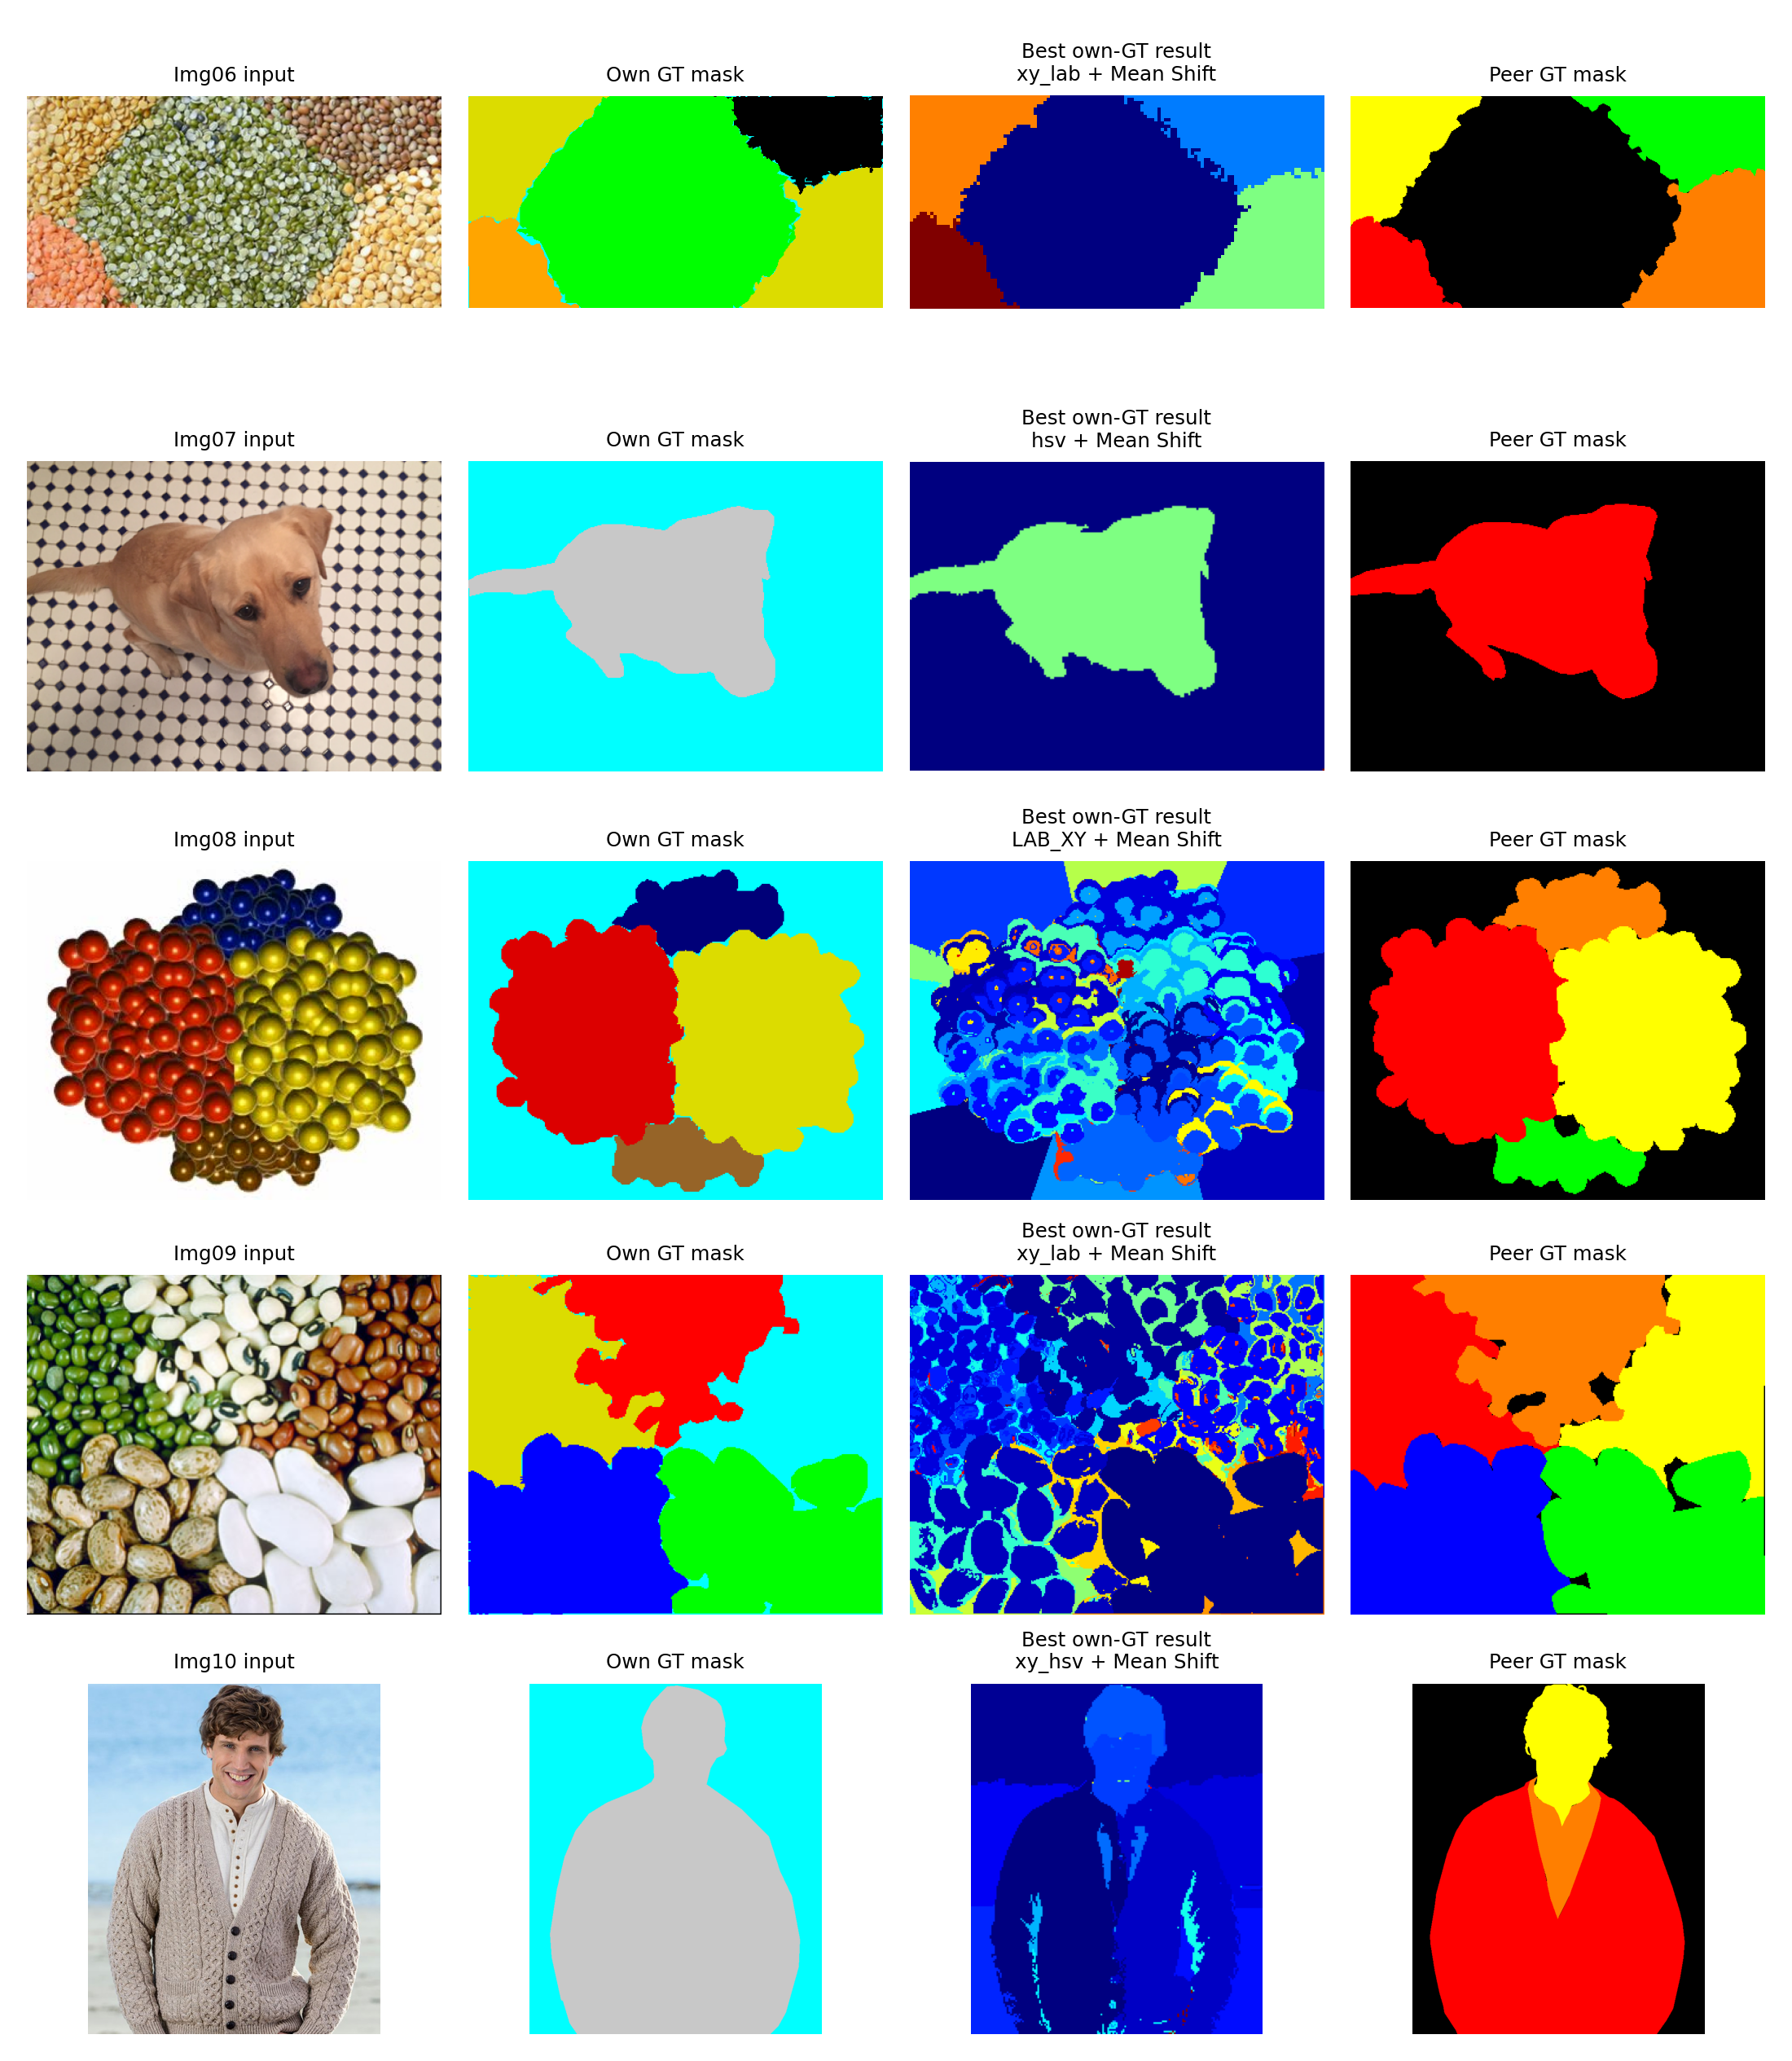
\includegraphics[width=0.95\textwidth,height=0.43\textheight,keepaspectratio]{figures/grids/best_qualitative_results_part2.png}
\caption{Best qualitative segmentation examples for Images 06--10, selected per image using own-GT macro IoU.}
\label{fig:best-qualitative-b}
\end{figure}

\subsection{Quantitative summary}
Across all 478 post-processed outputs, the overall macro Precision is 0.588, macro Recall is 0.601, macro IoU is 0.498, and macro Boundary F1-score is 0.257. These averages include deliberately weak feature spaces, under-segmented outputs, over-segmented outputs, and multiple Mean Shift bandwidths, so they represent the full experimental sweep rather than only the best cases.

\begin{figure}[H]
\centering
\begin{subfigure}{0.48\textwidth}
\centering
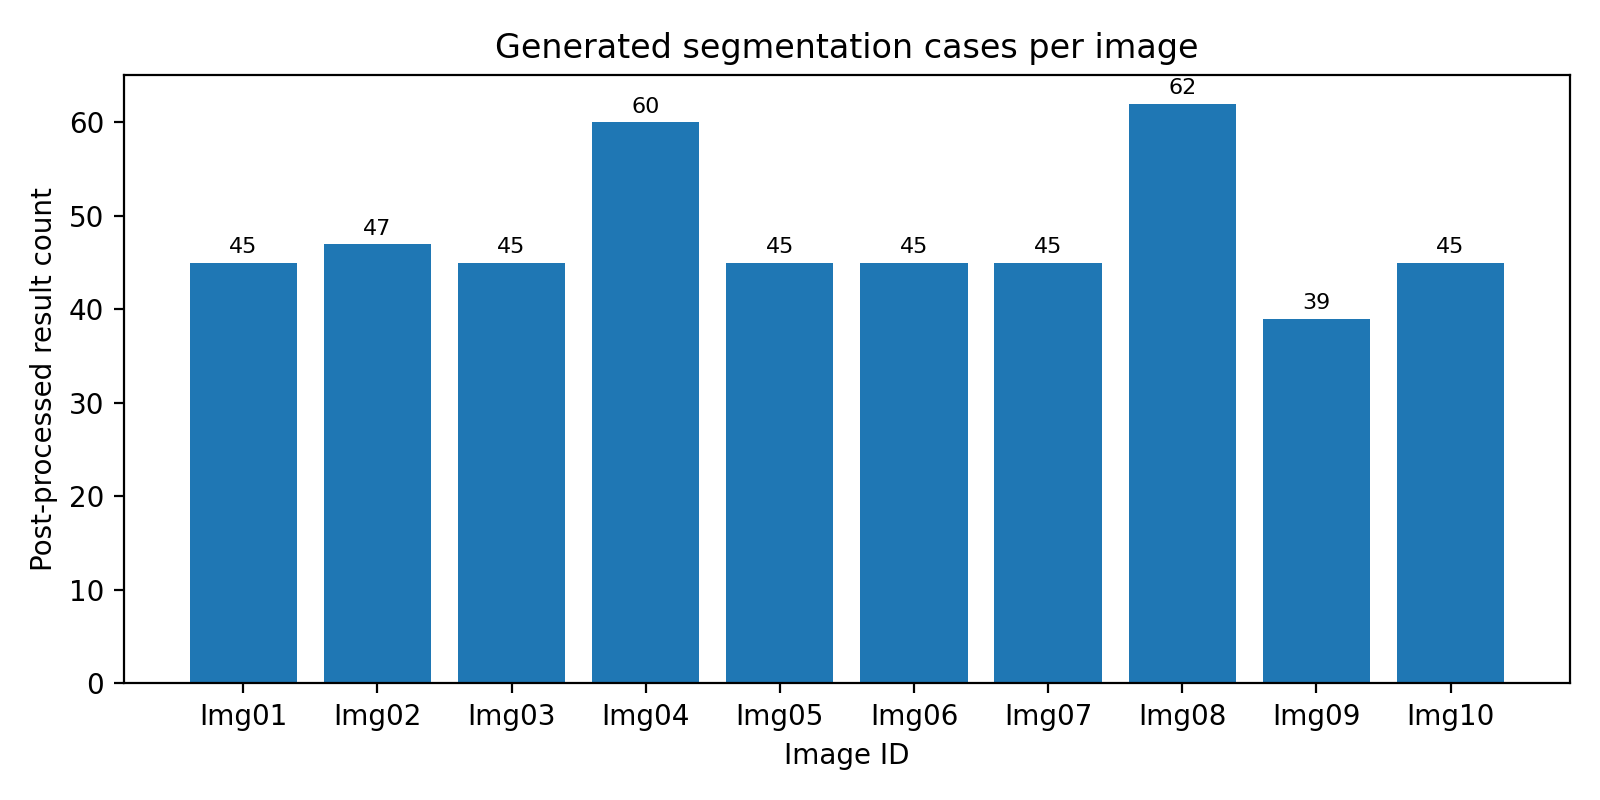
\includegraphics[width=\textwidth]{figures/charts/output_count_by_image.png}
\caption{Number of generated result cases per image.}
\end{subfigure}\hfill
\begin{subfigure}{0.48\textwidth}
\centering
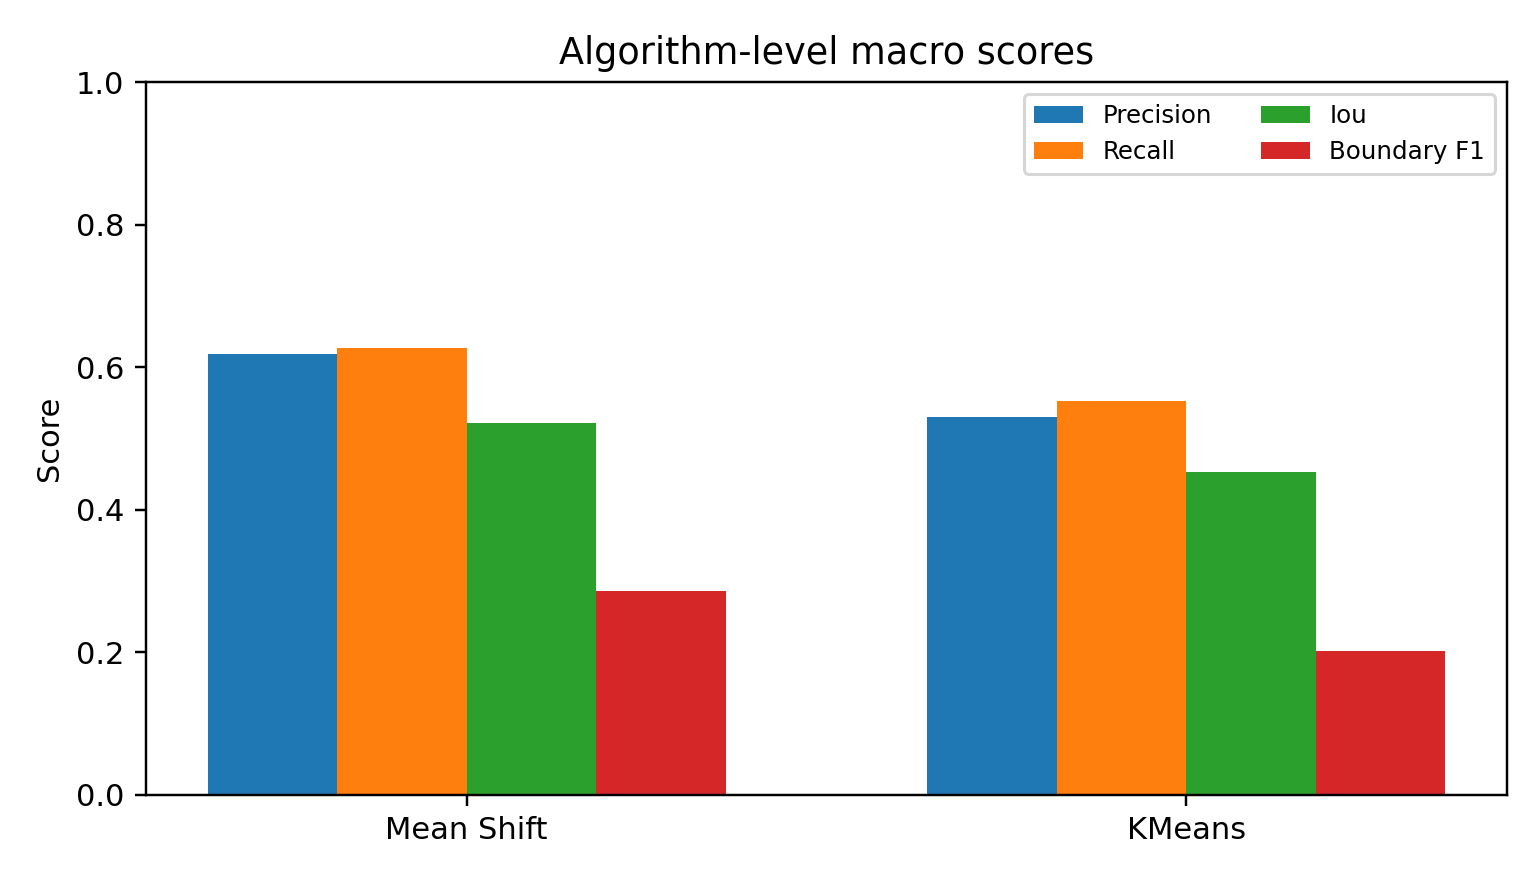
\includegraphics[width=\textwidth]{figures/charts/algorithm_summary_metrics.png}
\caption{Macro scores grouped by algorithm.}
\end{subfigure}
\caption{Quantitative overview of the complete experiment.}
\label{fig:quant-overview}
\end{figure}

\begin{table}[H]
\centering
\caption{Algorithm-level quantitative results over the generated outputs.}
\resizebox{\textwidth}{!}{%
\begin{tabular}{@{}lrrrrrr@{}}
\toprule
Algorithm & Cases & Images & Prec. & Recall & IoU & BF \\
\midrule
Mean Shift & 314 & 10 & 0.619 & 0.626 & 0.521 & 0.285 \\
KMeans & 164 & 10 & 0.530 & 0.553 & 0.454 & 0.202 \\
\bottomrule
\end{tabular}
}
\label{tab:algorithm-results}
\end{table}

\subsection{Best feature-space groups}
The strongest feature-space groups combine spatial coordinates with Lab or HSV color, and in some cases texture. This supports the design idea: spatial features improve compactness, while perceptual color spaces make the clusters more meaningful than raw RGB alone.

\begin{figure}[H]
\centering
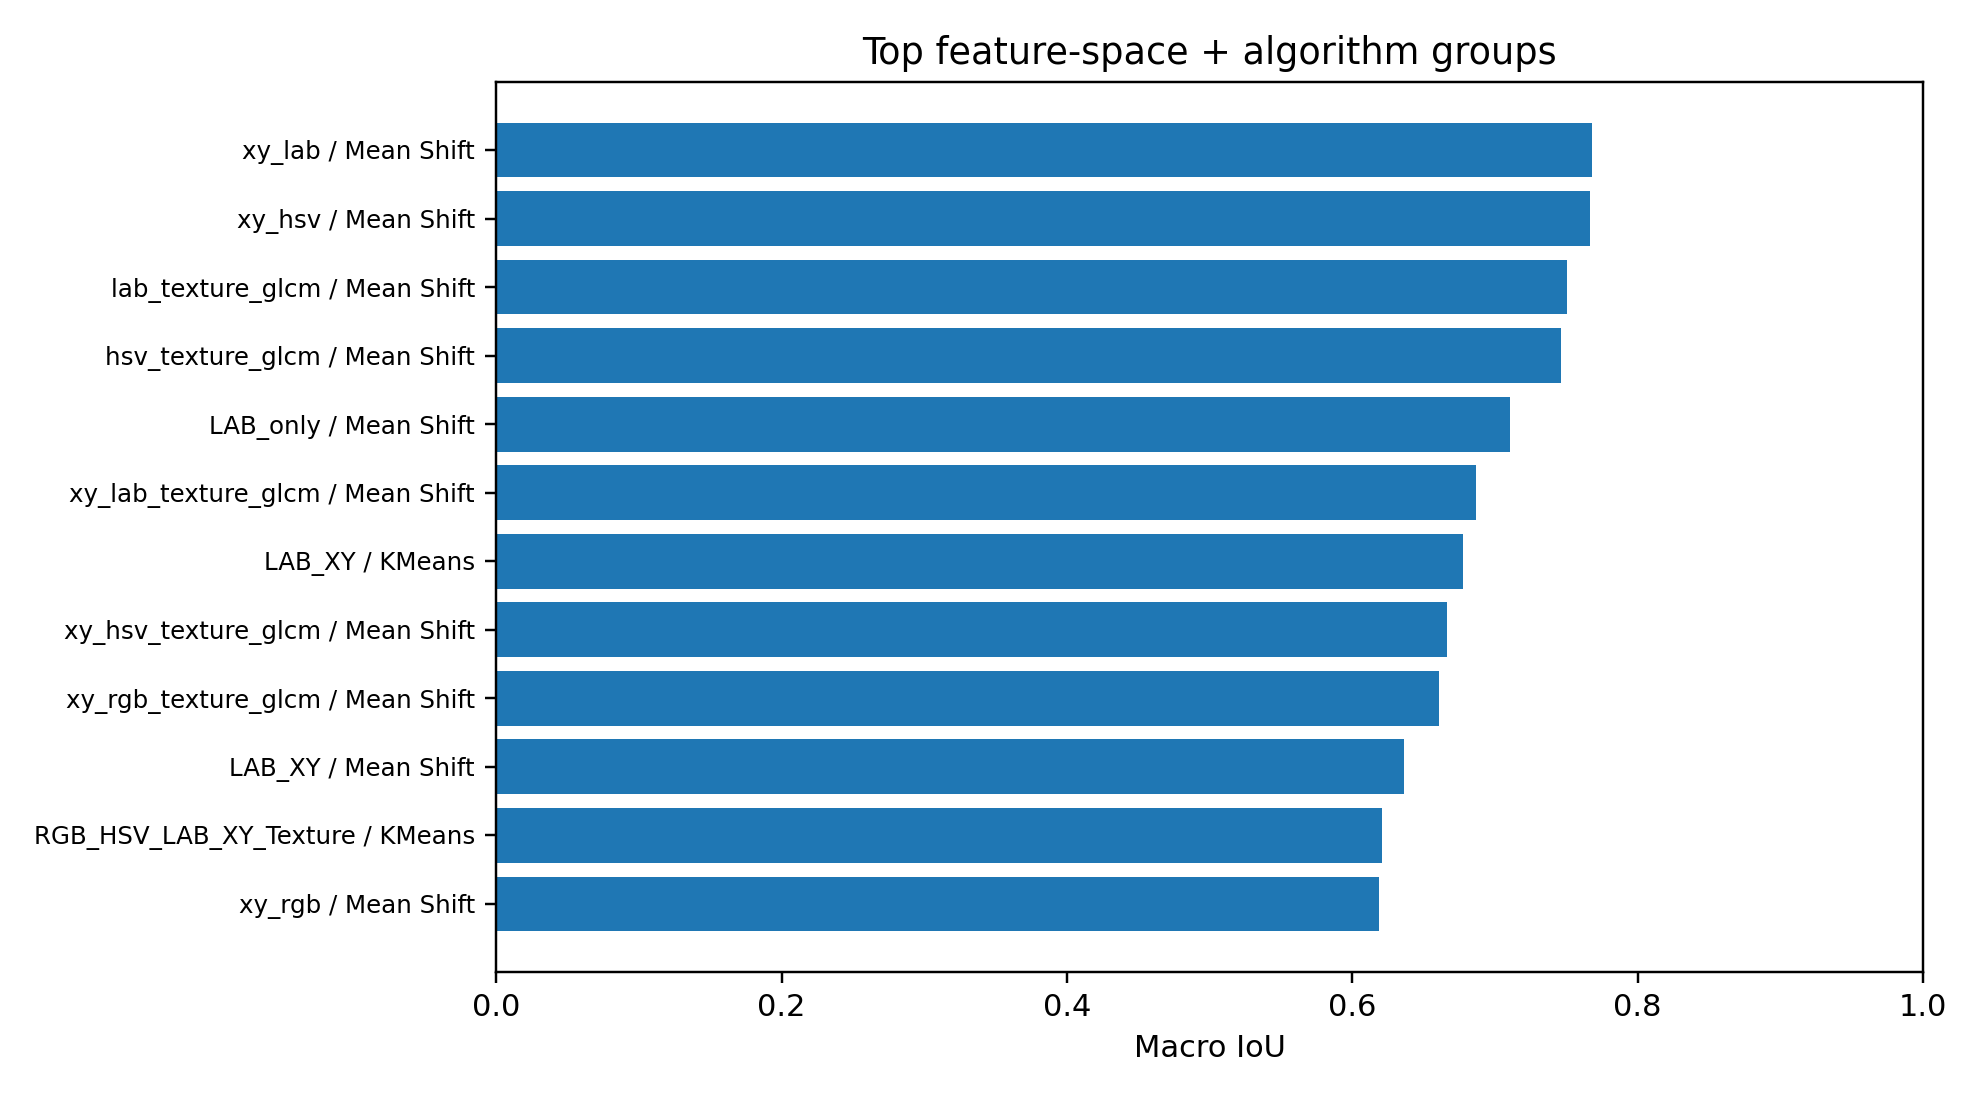
\includegraphics[width=0.9\textwidth]{figures/charts/top_feature_algorithm_macro_iou.png}
\caption{Top feature-space and algorithm groups ranked by macro IoU.}
\label{fig:top-feature-algorithm}
\end{figure}

\begin{table}[H]
\centering
\caption{Top feature-space and algorithm groups by macro IoU.}
\resizebox{\textwidth}{!}{%
\begin{tabular}{@{}lrrrrrrr@{}}
\toprule
Feature set & Alg. & Cases & Images & Prec. & Recall & IoU & BF \\
\midrule
xy\_lab & Mean Shift & 18 & 9 & 0.825 & 0.821 & 0.768 & 0.514 \\
xy\_hsv & Mean Shift & 18 & 9 & 0.833 & 0.825 & 0.767 & 0.501 \\
lab\_texture\_glcm & Mean Shift & 6 & 3 & 0.848 & 0.796 & 0.750 & 0.446 \\
hsv\_texture\_glcm & Mean Shift & 6 & 3 & 0.822 & 0.816 & 0.746 & 0.434 \\
LAB\_only & Mean Shift & 6 & 1 & 0.747 & 0.789 & 0.711 & 0.552 \\
xy\_lab\_texture\_glcm & Mean Shift & 6 & 3 & 0.800 & 0.741 & 0.687 & 0.430 \\
LAB\_XY & KMeans & 1 & 1 & 0.699 & 0.727 & 0.678 & 0.482 \\
xy\_hsv\_texture\_glcm & Mean Shift & 6 & 3 & 0.820 & 0.731 & 0.666 & 0.429 \\
\bottomrule
\end{tabular}
}
\label{tab:top-feature-algorithm}
\end{table}

\subsection{Representative normalized confusion matrix}
The normalized confusion matrix in \Cref{fig:representative-cm} shows a representative best-scoring result. Values on the diagonal correspond to correctly matched GT classes, while off-diagonal entries show class confusion after label matching. The complete long-form normalized confusion matrices are included in \texttt{numerical\_results/own\_gt/confusion\_matrices\_long.csv}.

\begin{figure}[H]
\centering
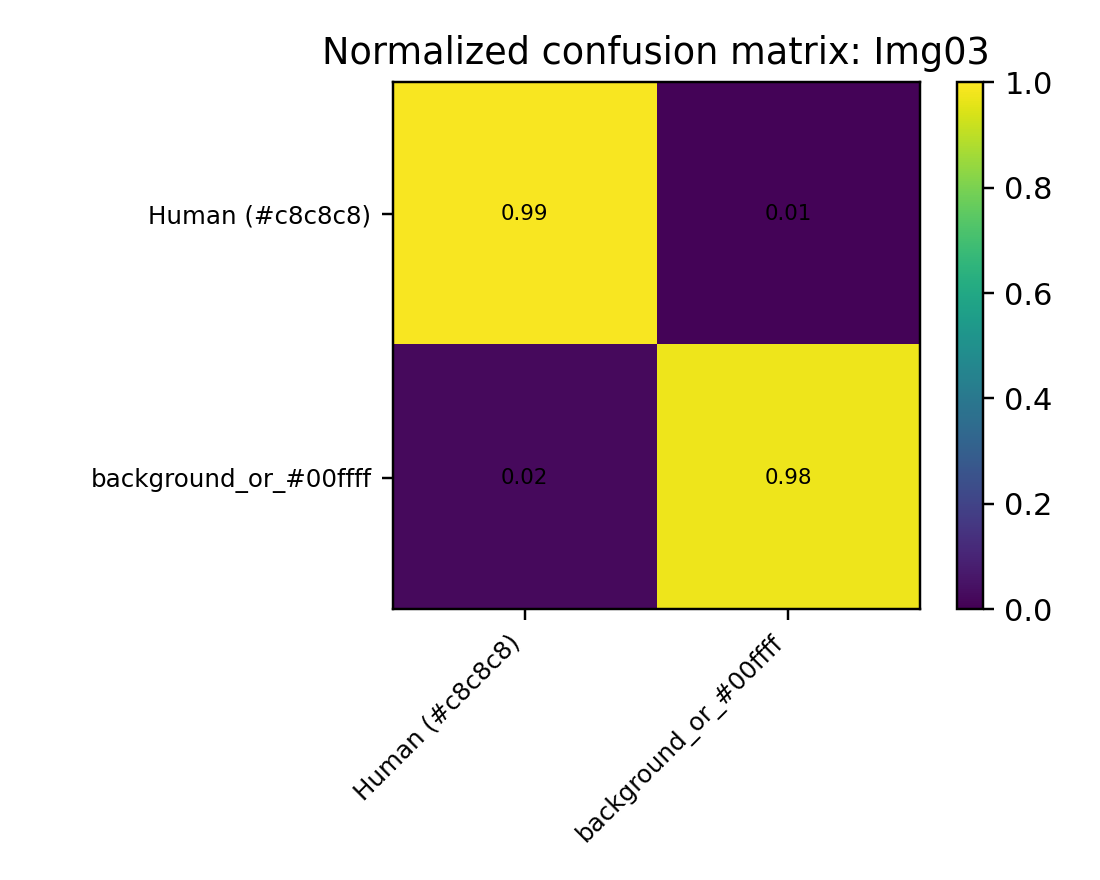
\includegraphics[width=0.58\textwidth]{figures/charts/representative_confusion_matrix.png}
\caption{Representative row-normalized confusion matrix after many-to-one label matching.}
\label{fig:representative-cm}
\end{figure}

\subsection{Discussion}
Several trends are visible in the output tables and figures. First, XY combined with Lab or HSV is consistently strong, because it balances color discrimination with spatial coherence. Second, texture-only features can be useful when surface pattern dominates, but they may be unstable when the image contains smooth regions or when Mean Shift produces too many small modes. Third, K-means is fast and stable but depends on a chosen $K$, while Mean Shift can adapt cluster count but needs careful bandwidth, sampling, resizing, or PCA. Finally, post-processing improves visual smoothness by removing isolated components, which is important because unsupervised clustering often produces small noisy islands.


\section{Peer Ground Truth Evaluation}
The assignment also asks for testing with at least one peer's GT. The peer masks and annotation JSON files are included in \texttt{peer\_ground\_truth\_images/} and also copied into \texttt{outputs/Peer GT/} in the same format as the self GT. Because a full peer comparison was not originally completed, this package adds an additional numerical peer-GT evaluation.

The protocol is: for each image, select the strongest prediction according to own-GT macro IoU, then evaluate that prediction against the peer GT using the same many-to-one label matching and metric definitions. This is a fair late-stage peer test because it does not tune parameters on peer labels; it uses the already selected best result and checks how well it agrees with another annotator.

\begin{figure}[H]
\centering
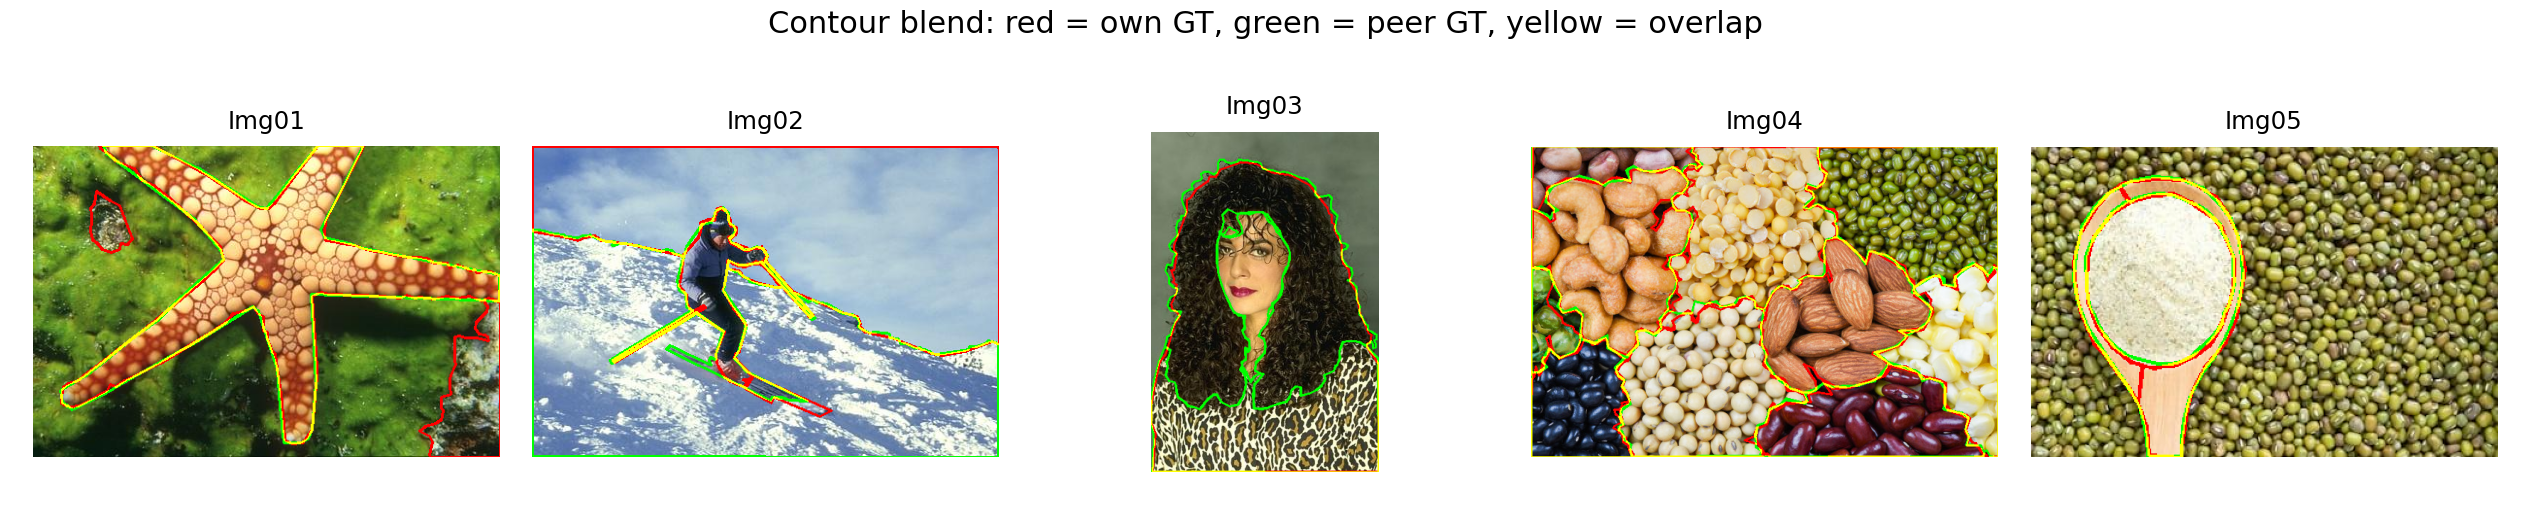
\includegraphics[width=0.95\textwidth,height=0.30\textheight,keepaspectratio]{figures/grids/peer_contour_blend_part1.png}
\caption{Self-vs-peer contour blends for Images 01--05. Red shows the self GT contour, green shows the peer GT contour, and yellow indicates overlap.}
\label{fig:peer-contour-blend-a}
\end{figure}
\begin{figure}[H]
\centering
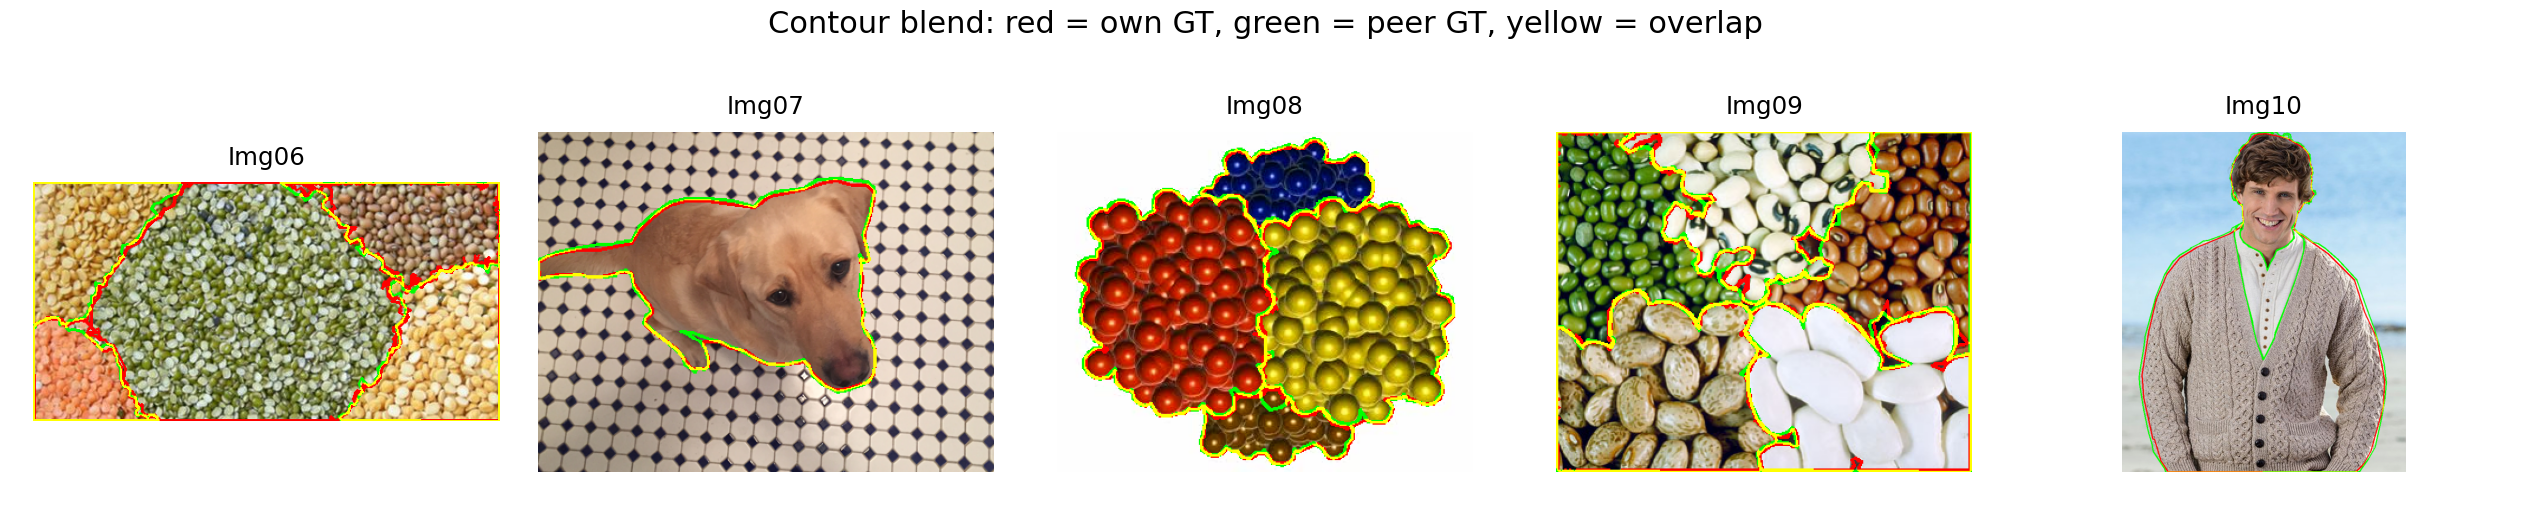
\includegraphics[width=0.95\textwidth,height=0.30\textheight,keepaspectratio]{figures/grids/peer_contour_blend_part2.png}
\caption{Self-vs-peer contour blends for Images 06--10.}
\label{fig:peer-contour-blend-b}
\end{figure}

\begin{figure}[H]
\centering
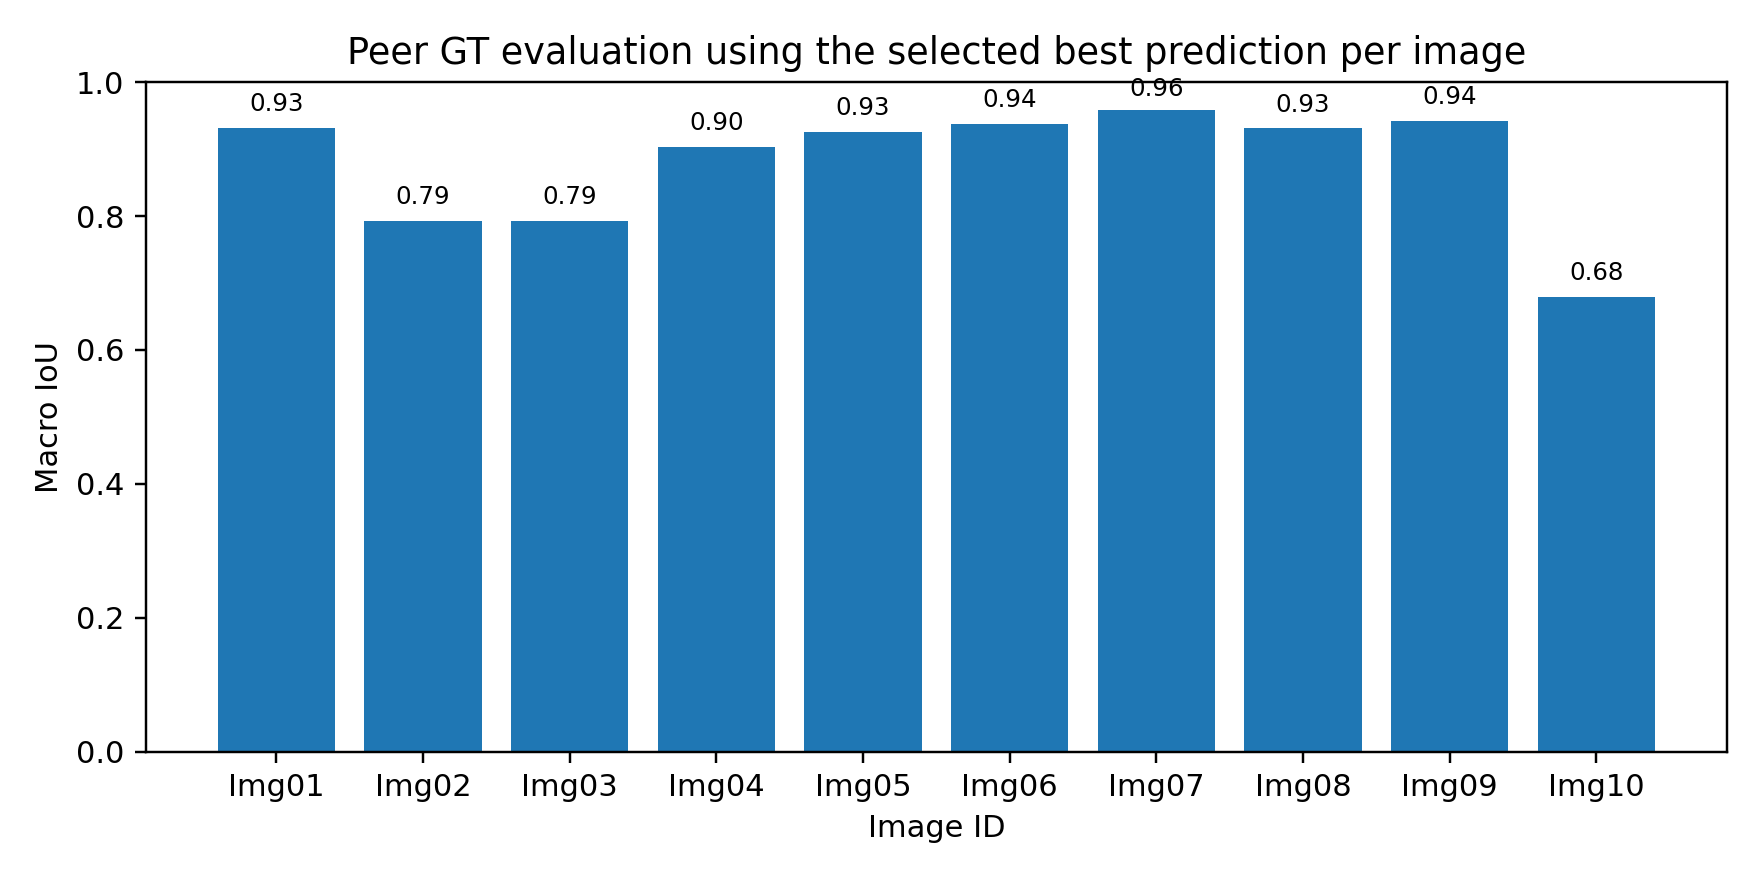
\includegraphics[width=0.82\textwidth]{figures/charts/peer_best_iou_by_image.png}
\caption{Macro IoU against peer GT using the selected best prediction per image.}
\label{fig:peer-iou}
\end{figure}

The peer-GT evaluation over ten images obtains macro Precision 0.958, macro Recall 0.917, macro IoU 0.880, and macro Boundary F1-score 0.681. The detailed per-image peer results are stored in \texttt{numerical\_results/peer\_gt/peer\_best\_per\_image\_results.csv}.

\begin{table}[H]
\centering
\caption{Peer-GT numerical results for the selected best prediction per image.}
\resizebox{\textwidth}{!}{%
\begin{tabular}{@{}lrrrrrr@{}}
\toprule
Image & Feature & Alg. & Prec. & Recall & IoU & BF \\
\midrule
Img01 & xy\_hsv & Mean Shift & 0.972 & 0.958 & 0.932 & 0.781 \\
Img02 & xy\_lab & Mean Shift & 0.945 & 0.836 & 0.793 & 0.532 \\
Img03 & hsv & Mean Shift & 0.924 & 0.856 & 0.793 & 0.344 \\
Img04 & xy\_lab & Mean Shift & 0.933 & 0.965 & 0.904 & 0.615 \\
Img05 & lab & Mean Shift & 0.953 & 0.970 & 0.926 & 0.904 \\
Img06 & xy\_lab & Mean Shift & 0.957 & 0.979 & 0.937 & 0.769 \\
Img07 & hsv & Mean Shift & 0.991 & 0.966 & 0.958 & 0.833 \\
Img08 & LAB\_XY & Mean Shift & 0.970 & 0.959 & 0.931 & 0.889 \\
Img09 & xy\_lab & Mean Shift & 0.961 & 0.980 & 0.942 & 0.778 \\
Img10 & xy\_hsv & Mean Shift & 0.971 & 0.706 & 0.680 & 0.361 \\
\bottomrule
\end{tabular}
}
\label{tab:peer-results}
\end{table}

The contour blend indicates that the largest disagreements usually occur at ambiguous boundaries or thin structures. This is expected because manual polygon annotations from two people rarely match perfectly. The high peer macro IoU still suggests that the selected segmentations are not merely overfitting one annotation set; they are broadly consistent with another GT interpretation.


\section{Conclusion}
This project presents a complete segmentation workflow from manual annotation to quantitative evaluation. The proposed idea is to convert pixels into adaptive feature spaces that combine spatial position, color, and texture, then apply K-means and Mean Shift clustering with practical speed controls such as sampling, resizing, and PCA. The final package includes all required materials: GT masks/contours/overlays, peer GT, annotation JSON files, program files, full output images, and CSV results.

The experiments show that color-space and spatial combinations, especially XY + Lab and XY + HSV with Mean Shift, are strong choices for this image set. Texture features are valuable but should be selected carefully according to image content, since high-dimensional filter responses can make Mean Shift slower and sometimes less stable. The added peer-GT evaluation provides an extra check of annotation robustness and shows that the selected best outputs remain strong against another annotator's masks.

Future improvements would include a fully unified Gaussian/Epanechnikov Mean Shift implementation for all images, automatic bandwidth selection, and a deeper comparison between Gabor, Leung--Malik, GLCM, and learned texture descriptors such as DINO-style features.


\bibliographystyle{plainnat}
\bibliography{references}

\appendix

\section{Head Views of Important Files}
This appendix shows small previews of important files. The full files are included in the project folders.

\subsection{Project folder head}
\lstinputlisting{materials/head_views/project_tree_head.txt}

\subsection{Annotation JSON head}
\lstinputlisting{materials/head_views/annotation_head_Img01.json}

\subsection{Program feature-menu head}
\lstinputlisting[language=Python]{materials/head_views/program_feature_menu_head.py}

\subsection{Per-image result CSV head}
\lstinputlisting{materials/head_views/per_image_results_head.csv}

\subsection{Feature/algorithm summary CSV head}
\lstinputlisting{materials/head_views/macro_by_feature_algorithm_head.csv}

\subsection{Peer result CSV head}
\lstinputlisting{materials/head_views/peer_best_results_head.csv}

\section{Ground Truth Gallery}

All self and peer GT files are stored in the project folders. The following figures show the image, mask, contour, and overlay for each GT set.

\begin{figure}[H]
\centering
\begin{minipage}{0.23\textwidth}
\centering

\includegraphics[width=\linewidth]{\detokenize{outputs/Img01/Img01.jpg}}
\caption*{\scriptsize Input}
\end{minipage}\hfill
\begin{minipage}{0.23\textwidth}
\centering

\includegraphics[width=\linewidth]{\detokenize{outputs/GT Ehsanul Karim/Img01/mask.png}}
\caption*{\scriptsize Own mask}
\end{minipage}\hfill
\begin{minipage}{0.23\textwidth}
\centering

\includegraphics[width=\linewidth]{\detokenize{outputs/GT Ehsanul Karim/Img01/contour.png}}
\caption*{\scriptsize Own contour}
\end{minipage}\hfill
\begin{minipage}{0.23\textwidth}
\centering

\includegraphics[width=\linewidth]{\detokenize{outputs/GT Ehsanul Karim/Img01/contour_overlay.png}}
\caption*{\scriptsize Own overlay}
\end{minipage}\hfill
\caption{Self ground truth products for Img01.}
\label{fig:own-gt-Img01}
\end{figure}

\begin{figure}[H]
\centering
\begin{minipage}{0.23\textwidth}
\centering

\includegraphics[width=\linewidth]{\detokenize{outputs/Img02/Img02.jpg}}
\caption*{\scriptsize Input}
\end{minipage}\hfill
\begin{minipage}{0.23\textwidth}
\centering

\includegraphics[width=\linewidth]{\detokenize{outputs/GT Ehsanul Karim/Img02/mask.png}}
\caption*{\scriptsize Own mask}
\end{minipage}\hfill
\begin{minipage}{0.23\textwidth}
\centering

\includegraphics[width=\linewidth]{\detokenize{outputs/GT Ehsanul Karim/Img02/contour.png}}
\caption*{\scriptsize Own contour}
\end{minipage}\hfill
\begin{minipage}{0.23\textwidth}
\centering

\includegraphics[width=\linewidth]{\detokenize{outputs/GT Ehsanul Karim/Img02/contour_overlay.png}}
\caption*{\scriptsize Own overlay}
\end{minipage}\hfill
\caption{Self ground truth products for Img02.}
\label{fig:own-gt-Img02}
\end{figure}

\begin{figure}[H]
\centering
\begin{minipage}{0.23\textwidth}
\centering

\includegraphics[width=\linewidth]{\detokenize{outputs/Img03/Img03.jpg}}
\caption*{\scriptsize Input}
\end{minipage}\hfill
\begin{minipage}{0.23\textwidth}
\centering

\includegraphics[width=\linewidth]{\detokenize{outputs/GT Ehsanul Karim/Img03/mask.png}}
\caption*{\scriptsize Own mask}
\end{minipage}\hfill
\begin{minipage}{0.23\textwidth}
\centering

\includegraphics[width=\linewidth]{\detokenize{outputs/GT Ehsanul Karim/Img03/contour.png}}
\caption*{\scriptsize Own contour}
\end{minipage}\hfill
\begin{minipage}{0.23\textwidth}
\centering

\includegraphics[width=\linewidth]{\detokenize{outputs/GT Ehsanul Karim/Img03/contour_overlay.png}}
\caption*{\scriptsize Own overlay}
\end{minipage}\hfill
\caption{Self ground truth products for Img03.}
\label{fig:own-gt-Img03}
\end{figure}

\begin{figure}[H]
\centering
\begin{minipage}{0.23\textwidth}
\centering

\includegraphics[width=\linewidth]{\detokenize{outputs/Img04/Img04.jpg}}
\caption*{\scriptsize Input}
\end{minipage}\hfill
\begin{minipage}{0.23\textwidth}
\centering

\includegraphics[width=\linewidth]{\detokenize{outputs/GT Ehsanul Karim/Img04/mask.png}}
\caption*{\scriptsize Own mask}
\end{minipage}\hfill
\begin{minipage}{0.23\textwidth}
\centering

\includegraphics[width=\linewidth]{\detokenize{outputs/GT Ehsanul Karim/Img04/contour.png}}
\caption*{\scriptsize Own contour}
\end{minipage}\hfill
\begin{minipage}{0.23\textwidth}
\centering

\includegraphics[width=\linewidth]{\detokenize{outputs/GT Ehsanul Karim/Img04/contour_overlay.png}}
\caption*{\scriptsize Own overlay}
\end{minipage}\hfill
\caption{Self ground truth products for Img04.}
\label{fig:own-gt-Img04}
\end{figure}

\begin{figure}[H]
\centering
\begin{minipage}{0.23\textwidth}
\centering

\includegraphics[width=\linewidth]{\detokenize{outputs/Img05/Img05.jpg}}
\caption*{\scriptsize Input}
\end{minipage}\hfill
\begin{minipage}{0.23\textwidth}
\centering

\includegraphics[width=\linewidth]{\detokenize{outputs/GT Ehsanul Karim/Img05/mask.png}}
\caption*{\scriptsize Own mask}
\end{minipage}\hfill
\begin{minipage}{0.23\textwidth}
\centering

\includegraphics[width=\linewidth]{\detokenize{outputs/GT Ehsanul Karim/Img05/contour.png}}
\caption*{\scriptsize Own contour}
\end{minipage}\hfill
\begin{minipage}{0.23\textwidth}
\centering

\includegraphics[width=\linewidth]{\detokenize{outputs/GT Ehsanul Karim/Img05/contour_overlay.png}}
\caption*{\scriptsize Own overlay}
\end{minipage}\hfill
\caption{Self ground truth products for Img05.}
\label{fig:own-gt-Img05}
\end{figure}

\begin{figure}[H]
\centering
\begin{minipage}{0.23\textwidth}
\centering

\includegraphics[width=\linewidth]{\detokenize{outputs/Img06/Img06.jpg}}
\caption*{\scriptsize Input}
\end{minipage}\hfill
\begin{minipage}{0.23\textwidth}
\centering

\includegraphics[width=\linewidth]{\detokenize{outputs/GT Ehsanul Karim/Img06/mask.png}}
\caption*{\scriptsize Own mask}
\end{minipage}\hfill
\begin{minipage}{0.23\textwidth}
\centering

\includegraphics[width=\linewidth]{\detokenize{outputs/GT Ehsanul Karim/Img06/contour.png}}
\caption*{\scriptsize Own contour}
\end{minipage}\hfill
\begin{minipage}{0.23\textwidth}
\centering

\includegraphics[width=\linewidth]{\detokenize{outputs/GT Ehsanul Karim/Img06/contour_overlay.png}}
\caption*{\scriptsize Own overlay}
\end{minipage}\hfill
\caption{Self ground truth products for Img06.}
\label{fig:own-gt-Img06}
\end{figure}

\begin{figure}[H]
\centering
\begin{minipage}{0.23\textwidth}
\centering

\includegraphics[width=\linewidth]{\detokenize{outputs/Img07/Img07.png}}
\caption*{\scriptsize Input}
\end{minipage}\hfill
\begin{minipage}{0.23\textwidth}
\centering

\includegraphics[width=\linewidth]{\detokenize{outputs/GT Ehsanul Karim/Img07/mask.png}}
\caption*{\scriptsize Own mask}
\end{minipage}\hfill
\begin{minipage}{0.23\textwidth}
\centering

\includegraphics[width=\linewidth]{\detokenize{outputs/GT Ehsanul Karim/Img07/contour.png}}
\caption*{\scriptsize Own contour}
\end{minipage}\hfill
\begin{minipage}{0.23\textwidth}
\centering

\includegraphics[width=\linewidth]{\detokenize{outputs/GT Ehsanul Karim/Img07/contour_overlay.png}}
\caption*{\scriptsize Own overlay}
\end{minipage}\hfill
\caption{Self ground truth products for Img07.}
\label{fig:own-gt-Img07}
\end{figure}

\begin{figure}[H]
\centering
\begin{minipage}{0.23\textwidth}
\centering

\includegraphics[width=\linewidth]{\detokenize{outputs/Img08/Img08.jpg}}
\caption*{\scriptsize Input}
\end{minipage}\hfill
\begin{minipage}{0.23\textwidth}
\centering

\includegraphics[width=\linewidth]{\detokenize{outputs/GT Ehsanul Karim/Img08/mask.png}}
\caption*{\scriptsize Own mask}
\end{minipage}\hfill
\begin{minipage}{0.23\textwidth}
\centering

\includegraphics[width=\linewidth]{\detokenize{outputs/GT Ehsanul Karim/Img08/contour.png}}
\caption*{\scriptsize Own contour}
\end{minipage}\hfill
\begin{minipage}{0.23\textwidth}
\centering

\includegraphics[width=\linewidth]{\detokenize{outputs/GT Ehsanul Karim/Img08/contour_overlay.png}}
\caption*{\scriptsize Own overlay}
\end{minipage}\hfill
\caption{Self ground truth products for Img08.}
\label{fig:own-gt-Img08}
\end{figure}

\begin{figure}[H]
\centering
\begin{minipage}{0.23\textwidth}
\centering

\includegraphics[width=\linewidth]{\detokenize{outputs/Img09/Img09.png}}
\caption*{\scriptsize Input}
\end{minipage}\hfill
\begin{minipage}{0.23\textwidth}
\centering

\includegraphics[width=\linewidth]{\detokenize{outputs/GT Ehsanul Karim/Img09/mask.png}}
\caption*{\scriptsize Own mask}
\end{minipage}\hfill
\begin{minipage}{0.23\textwidth}
\centering

\includegraphics[width=\linewidth]{\detokenize{outputs/GT Ehsanul Karim/Img09/contour.png}}
\caption*{\scriptsize Own contour}
\end{minipage}\hfill
\begin{minipage}{0.23\textwidth}
\centering

\includegraphics[width=\linewidth]{\detokenize{outputs/GT Ehsanul Karim/Img09/contour_overlay.png}}
\caption*{\scriptsize Own overlay}
\end{minipage}\hfill
\caption{Self ground truth products for Img09.}
\label{fig:own-gt-Img09}
\end{figure}

\begin{figure}[H]
\centering
\begin{minipage}{0.23\textwidth}
\centering

\includegraphics[width=\linewidth]{\detokenize{outputs/Img10/Img10.jpg}}
\caption*{\scriptsize Input}
\end{minipage}\hfill
\begin{minipage}{0.23\textwidth}
\centering

\includegraphics[width=\linewidth]{\detokenize{outputs/GT Ehsanul Karim/Img10/mask.png}}
\caption*{\scriptsize Own mask}
\end{minipage}\hfill
\begin{minipage}{0.23\textwidth}
\centering

\includegraphics[width=\linewidth]{\detokenize{outputs/GT Ehsanul Karim/Img10/contour.png}}
\caption*{\scriptsize Own contour}
\end{minipage}\hfill
\begin{minipage}{0.23\textwidth}
\centering

\includegraphics[width=\linewidth]{\detokenize{outputs/GT Ehsanul Karim/Img10/contour_overlay.png}}
\caption*{\scriptsize Own overlay}
\end{minipage}\hfill
\caption{Self ground truth products for Img10.}
\label{fig:own-gt-Img10}
\end{figure}

\begin{figure}[H]
\centering
\begin{minipage}{0.23\textwidth}
\centering
\includegraphics[width=\linewidth]{\detokenize{outputs/Peer GT/Img01/input.png}}
\caption*{\scriptsize Peer input}
\end{minipage}\hfill
\begin{minipage}{0.23\textwidth}
\centering

\includegraphics[width=\linewidth]{\detokenize{outputs/Peer GT/Img01/mask.png}}
\caption*{\scriptsize Peer mask}
\end{minipage}\hfill
\begin{minipage}{0.23\textwidth}
\centering

\includegraphics[width=\linewidth]{\detokenize{outputs/Peer GT/Img01/contour.png}}
\caption*{\scriptsize Peer contour}
\end{minipage}\hfill
\begin{minipage}{0.23\textwidth}
\centering

\includegraphics[width=\linewidth]{\detokenize{outputs/Peer GT/Img01/contour_overlay.png}}
\caption*{\scriptsize Peer overlay}
\end{minipage}\hfill
\caption{Peer ground truth products for Img01.}
\label{fig:peer-gt-Img01}
\end{figure}

\begin{figure}[H]
\centering
\begin{minipage}{0.23\textwidth}
\centering
\includegraphics[width=\linewidth]{\detokenize{outputs/Peer GT/Img02/input.png}}
\caption*{\scriptsize Peer input}
\end{minipage}\hfill
\begin{minipage}{0.23\textwidth}
\centering

\includegraphics[width=\linewidth]{\detokenize{outputs/Peer GT/Img02/mask.png}}
\caption*{\scriptsize Peer mask}
\end{minipage}\hfill
\begin{minipage}{0.23\textwidth}
\centering

\includegraphics[width=\linewidth]{\detokenize{outputs/Peer GT/Img02/contour.png}}
\caption*{\scriptsize Peer contour}
\end{minipage}\hfill
\begin{minipage}{0.23\textwidth}
\centering

\includegraphics[width=\linewidth]{\detokenize{outputs/Peer GT/Img02/contour_overlay.png}}
\caption*{\scriptsize Peer overlay}
\end{minipage}\hfill
\caption{Peer ground truth products for Img02.}
\label{fig:peer-gt-Img02}
\end{figure}

\begin{figure}[H]
\centering
\begin{minipage}{0.23\textwidth}
\centering
\includegraphics[width=\linewidth]{\detokenize{outputs/Peer GT/Img03/input.png}}
\caption*{\scriptsize Peer input}
\end{minipage}\hfill
\begin{minipage}{0.23\textwidth}
\centering

\includegraphics[width=\linewidth]{\detokenize{outputs/Peer GT/Img03/mask.png}}
\caption*{\scriptsize Peer mask}
\end{minipage}\hfill
\begin{minipage}{0.23\textwidth}
\centering

\includegraphics[width=\linewidth]{\detokenize{outputs/Peer GT/Img03/contour.png}}
\caption*{\scriptsize Peer contour}
\end{minipage}\hfill
\begin{minipage}{0.23\textwidth}
\centering

\includegraphics[width=\linewidth]{\detokenize{outputs/Peer GT/Img03/contour_overlay.png}}
\caption*{\scriptsize Peer overlay}
\end{minipage}\hfill
\caption{Peer ground truth products for Img03.}
\label{fig:peer-gt-Img03}
\end{figure}

\begin{figure}[H]
\centering
\begin{minipage}{0.23\textwidth}
\centering
\includegraphics[width=\linewidth]{\detokenize{outputs/Peer GT/Img04/input.png}}
\caption*{\scriptsize Peer input}
\end{minipage}\hfill
\begin{minipage}{0.23\textwidth}
\centering

\includegraphics[width=\linewidth]{\detokenize{outputs/Peer GT/Img04/mask.png}}
\caption*{\scriptsize Peer mask}
\end{minipage}\hfill
\begin{minipage}{0.23\textwidth}
\centering

\includegraphics[width=\linewidth]{\detokenize{outputs/Peer GT/Img04/contour.png}}
\caption*{\scriptsize Peer contour}
\end{minipage}\hfill
\begin{minipage}{0.23\textwidth}
\centering

\includegraphics[width=\linewidth]{\detokenize{outputs/Peer GT/Img04/contour_overlay.png}}
\caption*{\scriptsize Peer overlay}
\end{minipage}\hfill
\caption{Peer ground truth products for Img04.}
\label{fig:peer-gt-Img04}
\end{figure}

\begin{figure}[H]
\centering
\begin{minipage}{0.23\textwidth}
\centering
\includegraphics[width=\linewidth]{\detokenize{outputs/Peer GT/Img05/input.png}}
\caption*{\scriptsize Peer input}
\end{minipage}\hfill
\begin{minipage}{0.23\textwidth}
\centering

\includegraphics[width=\linewidth]{\detokenize{outputs/Peer GT/Img05/mask.png}}
\caption*{\scriptsize Peer mask}
\end{minipage}\hfill
\begin{minipage}{0.23\textwidth}
\centering

\includegraphics[width=\linewidth]{\detokenize{outputs/Peer GT/Img05/contour.png}}
\caption*{\scriptsize Peer contour}
\end{minipage}\hfill
\begin{minipage}{0.23\textwidth}
\centering

\includegraphics[width=\linewidth]{\detokenize{outputs/Peer GT/Img05/contour_overlay.png}}
\caption*{\scriptsize Peer overlay}
\end{minipage}\hfill
\caption{Peer ground truth products for Img05.}
\label{fig:peer-gt-Img05}
\end{figure}

\begin{figure}[H]
\centering
\begin{minipage}{0.23\textwidth}
\centering
\includegraphics[width=\linewidth]{\detokenize{outputs/Peer GT/Img06/input.png}}
\caption*{\scriptsize Peer input}
\end{minipage}\hfill
\begin{minipage}{0.23\textwidth}
\centering

\includegraphics[width=\linewidth]{\detokenize{outputs/Peer GT/Img06/mask.png}}
\caption*{\scriptsize Peer mask}
\end{minipage}\hfill
\begin{minipage}{0.23\textwidth}
\centering

\includegraphics[width=\linewidth]{\detokenize{outputs/Peer GT/Img06/contour.png}}
\caption*{\scriptsize Peer contour}
\end{minipage}\hfill
\begin{minipage}{0.23\textwidth}
\centering

\includegraphics[width=\linewidth]{\detokenize{outputs/Peer GT/Img06/contour_overlay.png}}
\caption*{\scriptsize Peer overlay}
\end{minipage}\hfill
\caption{Peer ground truth products for Img06.}
\label{fig:peer-gt-Img06}
\end{figure}

\begin{figure}[H]
\centering
\begin{minipage}{0.23\textwidth}
\centering
\includegraphics[width=\linewidth]{\detokenize{outputs/Peer GT/Img07/input.png}}
\caption*{\scriptsize Peer input}
\end{minipage}\hfill
\begin{minipage}{0.23\textwidth}
\centering

\includegraphics[width=\linewidth]{\detokenize{outputs/Peer GT/Img07/mask.png}}
\caption*{\scriptsize Peer mask}
\end{minipage}\hfill
\begin{minipage}{0.23\textwidth}
\centering

\includegraphics[width=\linewidth]{\detokenize{outputs/Peer GT/Img07/contour.png}}
\caption*{\scriptsize Peer contour}
\end{minipage}\hfill
\begin{minipage}{0.23\textwidth}
\centering

\includegraphics[width=\linewidth]{\detokenize{outputs/Peer GT/Img07/contour_overlay.png}}
\caption*{\scriptsize Peer overlay}
\end{minipage}\hfill
\caption{Peer ground truth products for Img07.}
\label{fig:peer-gt-Img07}
\end{figure}

\begin{figure}[H]
\centering
\begin{minipage}{0.23\textwidth}
\centering
\includegraphics[width=\linewidth]{\detokenize{outputs/Peer GT/Img08/input.png}}
\caption*{\scriptsize Peer input}
\end{minipage}\hfill
\begin{minipage}{0.23\textwidth}
\centering

\includegraphics[width=\linewidth]{\detokenize{outputs/Peer GT/Img08/mask.png}}
\caption*{\scriptsize Peer mask}
\end{minipage}\hfill
\begin{minipage}{0.23\textwidth}
\centering

\includegraphics[width=\linewidth]{\detokenize{outputs/Peer GT/Img08/contour.png}}
\caption*{\scriptsize Peer contour}
\end{minipage}\hfill
\begin{minipage}{0.23\textwidth}
\centering

\includegraphics[width=\linewidth]{\detokenize{outputs/Peer GT/Img08/contour_overlay.png}}
\caption*{\scriptsize Peer overlay}
\end{minipage}\hfill
\caption{Peer ground truth products for Img08.}
\label{fig:peer-gt-Img08}
\end{figure}

\begin{figure}[H]
\centering
\begin{minipage}{0.23\textwidth}
\centering
\includegraphics[width=\linewidth]{\detokenize{outputs/Peer GT/Img09/input.png}}
\caption*{\scriptsize Peer input}
\end{minipage}\hfill
\begin{minipage}{0.23\textwidth}
\centering

\includegraphics[width=\linewidth]{\detokenize{outputs/Peer GT/Img09/mask.png}}
\caption*{\scriptsize Peer mask}
\end{minipage}\hfill
\begin{minipage}{0.23\textwidth}
\centering

\includegraphics[width=\linewidth]{\detokenize{outputs/Peer GT/Img09/contour.png}}
\caption*{\scriptsize Peer contour}
\end{minipage}\hfill
\begin{minipage}{0.23\textwidth}
\centering

\includegraphics[width=\linewidth]{\detokenize{outputs/Peer GT/Img09/contour_overlay.png}}
\caption*{\scriptsize Peer overlay}
\end{minipage}\hfill
\caption{Peer ground truth products for Img09.}
\label{fig:peer-gt-Img09}
\end{figure}

\begin{figure}[H]
\centering
\begin{minipage}{0.23\textwidth}
\centering
\includegraphics[width=\linewidth]{\detokenize{outputs/Peer GT/Img10/input.png}}
\caption*{\scriptsize Peer input}
\end{minipage}\hfill
\begin{minipage}{0.23\textwidth}
\centering

\includegraphics[width=\linewidth]{\detokenize{outputs/Peer GT/Img10/mask.png}}
\caption*{\scriptsize Peer mask}
\end{minipage}\hfill
\begin{minipage}{0.23\textwidth}
\centering

\includegraphics[width=\linewidth]{\detokenize{outputs/Peer GT/Img10/contour.png}}
\caption*{\scriptsize Peer contour}
\end{minipage}\hfill
\begin{minipage}{0.23\textwidth}
\centering

\includegraphics[width=\linewidth]{\detokenize{outputs/Peer GT/Img10/contour_overlay.png}}
\caption*{\scriptsize Peer overlay}
\end{minipage}\hfill
\caption{Peer ground truth products for Img10.}
\label{fig:peer-gt-Img10}
\end{figure}
\ifincludeallresultgallery
  \section{Complete Post-Processed Output Gallery}
This appendix contains all 478 post-processed result figures available in the submitted output folder. Each caption lists the image ID, feature set, algorithm/mode, and saved prediction name.
\clearpage
\subsection{Img01}
\begin{figure}[p]
\centering
\begin{minipage}{0.31\textwidth}
\centering

\includegraphics[width=\linewidth,height=0.20\textheight,keepaspectratio]{\detokenize{outputs/Img01/hsv/KMeans/Postprocessed Img01-segment of 5.png}}
\caption*{\scriptsize hsv | KMeans | Postprocessed Img01-segment of 5}
\end{minipage}\hfill
\begin{minipage}{0.31\textwidth}
\centering

\includegraphics[width=\linewidth,height=0.20\textheight,keepaspectratio]{\detokenize{outputs/Img01/hsv/Half Resize PCA 95 Mean Shift/Post Processed Img01-meanshift-0.8.png}}
\caption*{\scriptsize hsv | Half Resize PCA 95 Mean Shift | Post Processed Img01-meanshift-0.8}
\end{minipage}\hfill
\begin{minipage}{0.31\textwidth}
\centering

\includegraphics[width=\linewidth,height=0.20\textheight,keepaspectratio]{\detokenize{outputs/Img01/hsv/Half Resize PCA 95 Mean Shift/Post Processed Img01-meanshift-1.5.png}}
\caption*{\scriptsize hsv | Half Resize PCA 95 Mean Shift | Post Processed Img01-meanshift-1.5}
\end{minipage}\hfill
\begin{minipage}{0.31\textwidth}
\centering

\includegraphics[width=\linewidth,height=0.20\textheight,keepaspectratio]{\detokenize{outputs/Img01/hsv_texture/KMeans/Postprocessed Img01-segment of 5.png}}
\caption*{\scriptsize hsv\_texture | KMeans | Postprocessed Img01-segment of 5}
\end{minipage}\hfill
\begin{minipage}{0.31\textwidth}
\centering

\includegraphics[width=\linewidth,height=0.20\textheight,keepaspectratio]{\detokenize{outputs/Img01/hsv_texture/Half Resize PCA 95 Mean Shift/Post Processed Img01-meanshift-0.8.png}}
\caption*{\scriptsize hsv\_texture | Half Resize PCA 95 Mean Shift | Post Processed Img01-meanshift-0.8}
\end{minipage}\hfill
\begin{minipage}{0.31\textwidth}
\centering

\includegraphics[width=\linewidth,height=0.20\textheight,keepaspectratio]{\detokenize{outputs/Img01/hsv_texture/Half Resize PCA 95 Mean Shift/Post Processed Img01-meanshift-1.5.png}}
\caption*{\scriptsize hsv\_texture | Half Resize PCA 95 Mean Shift | Post Processed Img01-meanshift-1.5}
\end{minipage}\hfill
\begin{minipage}{0.31\textwidth}
\centering

\includegraphics[width=\linewidth,height=0.20\textheight,keepaspectratio]{\detokenize{outputs/Img01/lab/KMeans/Postprocessed Img01-segment of 5.png}}
\caption*{\scriptsize lab | KMeans | Postprocessed Img01-segment of 5}
\end{minipage}\hfill
\begin{minipage}{0.31\textwidth}
\centering

\includegraphics[width=\linewidth,height=0.20\textheight,keepaspectratio]{\detokenize{outputs/Img01/lab/Half Resize PCA 95 Mean Shift/Post Processed Img01-meanshift-0.8.png}}
\caption*{\scriptsize lab | Half Resize PCA 95 Mean Shift | Post Processed Img01-meanshift-0.8}
\end{minipage}\hfill
\begin{minipage}{0.31\textwidth}
\centering

\includegraphics[width=\linewidth,height=0.20\textheight,keepaspectratio]{\detokenize{outputs/Img01/lab/Half Resize PCA 95 Mean Shift/Post Processed Img01-meanshift-1.5.png}}
\caption*{\scriptsize lab | Half Resize PCA 95 Mean Shift | Post Processed Img01-meanshift-1.5}
\end{minipage}\hfill
\caption{Post-processed segmentation outputs for Img01 (gallery part 1).}
\end{figure}
\FloatBarrier
\begin{figure}[p]
\centering
\begin{minipage}{0.31\textwidth}
\centering

\includegraphics[width=\linewidth,height=0.20\textheight,keepaspectratio]{\detokenize{outputs/Img01/lab_texture/KMeans/Postprocessed Img01-segment of 5.png}}
\caption*{\scriptsize lab\_texture | KMeans | Postprocessed Img01-segment of 5}
\end{minipage}\hfill
\begin{minipage}{0.31\textwidth}
\centering

\includegraphics[width=\linewidth,height=0.20\textheight,keepaspectratio]{\detokenize{outputs/Img01/lab_texture/Half Resize PCA 95 Mean Shift/Post Processed Img01-meanshift-0.8.png}}
\caption*{\scriptsize lab\_texture | Half Resize PCA 95 Mean Shift | Post Processed Img01-meanshift-0.8}
\end{minipage}\hfill
\begin{minipage}{0.31\textwidth}
\centering

\includegraphics[width=\linewidth,height=0.20\textheight,keepaspectratio]{\detokenize{outputs/Img01/lab_texture/Half Resize PCA 95 Mean Shift/Post Processed Img01-meanshift-1.5.png}}
\caption*{\scriptsize lab\_texture | Half Resize PCA 95 Mean Shift | Post Processed Img01-meanshift-1.5}
\end{minipage}\hfill
\begin{minipage}{0.31\textwidth}
\centering

\includegraphics[width=\linewidth,height=0.20\textheight,keepaspectratio]{\detokenize{outputs/Img01/rgb/KMeans/Postprocessed Img01-segment of 5.png}}
\caption*{\scriptsize rgb | KMeans | Postprocessed Img01-segment of 5}
\end{minipage}\hfill
\begin{minipage}{0.31\textwidth}
\centering

\includegraphics[width=\linewidth,height=0.20\textheight,keepaspectratio]{\detokenize{outputs/Img01/rgb/Half Resize PCA 95 Mean Shift/Post Processed Img01-meanshift-0.8.png}}
\caption*{\scriptsize rgb | Half Resize PCA 95 Mean Shift | Post Processed Img01-meanshift-0.8}
\end{minipage}\hfill
\begin{minipage}{0.31\textwidth}
\centering

\includegraphics[width=\linewidth,height=0.20\textheight,keepaspectratio]{\detokenize{outputs/Img01/rgb/Half Resize PCA 95 Mean Shift/Post Processed Img01-meanshift-1.5.png}}
\caption*{\scriptsize rgb | Half Resize PCA 95 Mean Shift | Post Processed Img01-meanshift-1.5}
\end{minipage}\hfill
\begin{minipage}{0.31\textwidth}
\centering

\includegraphics[width=\linewidth,height=0.20\textheight,keepaspectratio]{\detokenize{outputs/Img01/rgb_texture/KMeans/Postprocessed Img01-segment of 5.png}}
\caption*{\scriptsize rgb\_texture | KMeans | Postprocessed Img01-segment of 5}
\end{minipage}\hfill
\begin{minipage}{0.31\textwidth}
\centering

\includegraphics[width=\linewidth,height=0.20\textheight,keepaspectratio]{\detokenize{outputs/Img01/rgb_texture/Half Resize PCA 95 Mean Shift/Post Processed Img01-meanshift-0.8.png}}
\caption*{\scriptsize rgb\_texture | Half Resize PCA 95 Mean Shift | Post Processed Img01-meanshift-0.8}
\end{minipage}\hfill
\begin{minipage}{0.31\textwidth}
\centering

\includegraphics[width=\linewidth,height=0.20\textheight,keepaspectratio]{\detokenize{outputs/Img01/rgb_texture/Half Resize PCA 95 Mean Shift/Post Processed Img01-meanshift-1.5.png}}
\caption*{\scriptsize rgb\_texture | Half Resize PCA 95 Mean Shift | Post Processed Img01-meanshift-1.5}
\end{minipage}\hfill
\caption{Post-processed segmentation outputs for Img01 (gallery part 2).}
\end{figure}
\FloatBarrier
\begin{figure}[p]
\centering
\begin{minipage}{0.31\textwidth}
\centering

\includegraphics[width=\linewidth,height=0.20\textheight,keepaspectratio]{\detokenize{outputs/Img01/texture/KMeans/Postprocessed Img01-segment of 5.png}}
\caption*{\scriptsize texture | KMeans | Postprocessed Img01-segment of 5}
\end{minipage}\hfill
\begin{minipage}{0.31\textwidth}
\centering

\includegraphics[width=\linewidth,height=0.20\textheight,keepaspectratio]{\detokenize{outputs/Img01/texture/Half Resize PCA 95 Mean Shift/Post Processed Img01-meanshift-0.8.png}}
\caption*{\scriptsize texture | Half Resize PCA 95 Mean Shift | Post Processed Img01-meanshift-0.8}
\end{minipage}\hfill
\begin{minipage}{0.31\textwidth}
\centering

\includegraphics[width=\linewidth,height=0.20\textheight,keepaspectratio]{\detokenize{outputs/Img01/texture/Half Resize PCA 95 Mean Shift/Post Processed Img01-meanshift-1.5.png}}
\caption*{\scriptsize texture | Half Resize PCA 95 Mean Shift | Post Processed Img01-meanshift-1.5}
\end{minipage}\hfill
\begin{minipage}{0.31\textwidth}
\centering

\includegraphics[width=\linewidth,height=0.20\textheight,keepaspectratio]{\detokenize{outputs/Img01/xy/KMeans/Postprocessed Img01-segment of 5.png}}
\caption*{\scriptsize xy | KMeans | Postprocessed Img01-segment of 5}
\end{minipage}\hfill
\begin{minipage}{0.31\textwidth}
\centering

\includegraphics[width=\linewidth,height=0.20\textheight,keepaspectratio]{\detokenize{outputs/Img01/xy/Half Resize PCA 95 Mean Shift/Post Processed Img01-meanshift-0.8.png}}
\caption*{\scriptsize xy | Half Resize PCA 95 Mean Shift | Post Processed Img01-meanshift-0.8}
\end{minipage}\hfill
\begin{minipage}{0.31\textwidth}
\centering

\includegraphics[width=\linewidth,height=0.20\textheight,keepaspectratio]{\detokenize{outputs/Img01/xy/Half Resize PCA 95 Mean Shift/Post Processed Img01-meanshift-1.5.png}}
\caption*{\scriptsize xy | Half Resize PCA 95 Mean Shift | Post Processed Img01-meanshift-1.5}
\end{minipage}\hfill
\begin{minipage}{0.31\textwidth}
\centering

\includegraphics[width=\linewidth,height=0.20\textheight,keepaspectratio]{\detokenize{outputs/Img01/xy_hsv/KMeans/Postprocessed Img01-segment of 5.png}}
\caption*{\scriptsize xy\_hsv | KMeans | Postprocessed Img01-segment of 5}
\end{minipage}\hfill
\begin{minipage}{0.31\textwidth}
\centering

\includegraphics[width=\linewidth,height=0.20\textheight,keepaspectratio]{\detokenize{outputs/Img01/xy_hsv/Half Resize PCA 95 Mean Shift/Post Processed Img01-meanshift-0.8.png}}
\caption*{\scriptsize xy\_hsv | Half Resize PCA 95 Mean Shift | Post Processed Img01-meanshift-0.8}
\end{minipage}\hfill
\begin{minipage}{0.31\textwidth}
\centering

\includegraphics[width=\linewidth,height=0.20\textheight,keepaspectratio]{\detokenize{outputs/Img01/xy_hsv/Half Resize PCA 95 Mean Shift/Post Processed Img01-meanshift-1.5.png}}
\caption*{\scriptsize xy\_hsv | Half Resize PCA 95 Mean Shift | Post Processed Img01-meanshift-1.5}
\end{minipage}\hfill
\caption{Post-processed segmentation outputs for Img01 (gallery part 3).}
\end{figure}
\FloatBarrier
\begin{figure}[p]
\centering
\begin{minipage}{0.31\textwidth}
\centering

\includegraphics[width=\linewidth,height=0.20\textheight,keepaspectratio]{\detokenize{outputs/Img01/xy_hsv_texture/KMeans/Postprocessed Img01-segment of 5.png}}
\caption*{\scriptsize xy\_hsv\_texture | KMeans | Postprocessed Img01-segment of 5}
\end{minipage}\hfill
\begin{minipage}{0.31\textwidth}
\centering

\includegraphics[width=\linewidth,height=0.20\textheight,keepaspectratio]{\detokenize{outputs/Img01/xy_hsv_texture/Half Resize PCA 95 Mean Shift/Post Processed Img01-meanshift-0.8.png}}
\caption*{\scriptsize xy\_hsv\_texture | Half Resize PCA 95 Mean Shift | Post Processed Img01-meanshift-0.8}
\end{minipage}\hfill
\begin{minipage}{0.31\textwidth}
\centering

\includegraphics[width=\linewidth,height=0.20\textheight,keepaspectratio]{\detokenize{outputs/Img01/xy_hsv_texture/Half Resize PCA 95 Mean Shift/Post Processed Img01-meanshift-1.5.png}}
\caption*{\scriptsize xy\_hsv\_texture | Half Resize PCA 95 Mean Shift | Post Processed Img01-meanshift-1.5}
\end{minipage}\hfill
\begin{minipage}{0.31\textwidth}
\centering

\includegraphics[width=\linewidth,height=0.20\textheight,keepaspectratio]{\detokenize{outputs/Img01/xy_lab/KMeans/Postprocessed Img01-segment of 5.png}}
\caption*{\scriptsize xy\_lab | KMeans | Postprocessed Img01-segment of 5}
\end{minipage}\hfill
\begin{minipage}{0.31\textwidth}
\centering

\includegraphics[width=\linewidth,height=0.20\textheight,keepaspectratio]{\detokenize{outputs/Img01/xy_lab/Half Resize PCA 95 Mean Shift/Post Processed Img01-meanshift-0.8.png}}
\caption*{\scriptsize xy\_lab | Half Resize PCA 95 Mean Shift | Post Processed Img01-meanshift-0.8}
\end{minipage}\hfill
\begin{minipage}{0.31\textwidth}
\centering

\includegraphics[width=\linewidth,height=0.20\textheight,keepaspectratio]{\detokenize{outputs/Img01/xy_lab/Half Resize PCA 95 Mean Shift/Post Processed Img01-meanshift-1.5.png}}
\caption*{\scriptsize xy\_lab | Half Resize PCA 95 Mean Shift | Post Processed Img01-meanshift-1.5}
\end{minipage}\hfill
\begin{minipage}{0.31\textwidth}
\centering

\includegraphics[width=\linewidth,height=0.20\textheight,keepaspectratio]{\detokenize{outputs/Img01/xy_lab_texture/KMeans/Postprocessed Img01-segment of 5.png}}
\caption*{\scriptsize xy\_lab\_texture | KMeans | Postprocessed Img01-segment of 5}
\end{minipage}\hfill
\begin{minipage}{0.31\textwidth}
\centering

\includegraphics[width=\linewidth,height=0.20\textheight,keepaspectratio]{\detokenize{outputs/Img01/xy_lab_texture/Half Resize PCA 95 Mean Shift/Post Processed Img01-meanshift-0.8.png}}
\caption*{\scriptsize xy\_lab\_texture | Half Resize PCA 95 Mean Shift | Post Processed Img01-meanshift-0.8}
\end{minipage}\hfill
\begin{minipage}{0.31\textwidth}
\centering

\includegraphics[width=\linewidth,height=0.20\textheight,keepaspectratio]{\detokenize{outputs/Img01/xy_lab_texture/Half Resize PCA 95 Mean Shift/Post Processed Img01-meanshift-1.5.png}}
\caption*{\scriptsize xy\_lab\_texture | Half Resize PCA 95 Mean Shift | Post Processed Img01-meanshift-1.5}
\end{minipage}\hfill
\caption{Post-processed segmentation outputs for Img01 (gallery part 4).}
\end{figure}
\FloatBarrier
\begin{figure}[p]
\centering
\begin{minipage}{0.31\textwidth}
\centering

\includegraphics[width=\linewidth,height=0.20\textheight,keepaspectratio]{\detokenize{outputs/Img01/xy_rgb/KMeans/Postprocessed Img01-segment of 5.png}}
\caption*{\scriptsize xy\_rgb | KMeans | Postprocessed Img01-segment of 5}
\end{minipage}\hfill
\begin{minipage}{0.31\textwidth}
\centering

\includegraphics[width=\linewidth,height=0.20\textheight,keepaspectratio]{\detokenize{outputs/Img01/xy_rgb/Half Resize PCA 95 Mean Shift/Post Processed Img01-meanshift-0.8.png}}
\caption*{\scriptsize xy\_rgb | Half Resize PCA 95 Mean Shift | Post Processed Img01-meanshift-0.8}
\end{minipage}\hfill
\begin{minipage}{0.31\textwidth}
\centering

\includegraphics[width=\linewidth,height=0.20\textheight,keepaspectratio]{\detokenize{outputs/Img01/xy_rgb/Half Resize PCA 95 Mean Shift/Post Processed Img01-meanshift-1.5.png}}
\caption*{\scriptsize xy\_rgb | Half Resize PCA 95 Mean Shift | Post Processed Img01-meanshift-1.5}
\end{minipage}\hfill
\begin{minipage}{0.31\textwidth}
\centering

\includegraphics[width=\linewidth,height=0.20\textheight,keepaspectratio]{\detokenize{outputs/Img01/xy_rgb_texture/KMeans/Postprocessed Img01-segment of 5.png}}
\caption*{\scriptsize xy\_rgb\_texture | KMeans | Postprocessed Img01-segment of 5}
\end{minipage}\hfill
\begin{minipage}{0.31\textwidth}
\centering

\includegraphics[width=\linewidth,height=0.20\textheight,keepaspectratio]{\detokenize{outputs/Img01/xy_rgb_texture/Half Resize PCA 95 Mean Shift/Post Processed Img01-meanshift-0.8.png}}
\caption*{\scriptsize xy\_rgb\_texture | Half Resize PCA 95 Mean Shift | Post Processed Img01-meanshift-0.8}
\end{minipage}\hfill
\begin{minipage}{0.31\textwidth}
\centering

\includegraphics[width=\linewidth,height=0.20\textheight,keepaspectratio]{\detokenize{outputs/Img01/xy_rgb_texture/Half Resize PCA 95 Mean Shift/Post Processed Img01-meanshift-1.5.png}}
\caption*{\scriptsize xy\_rgb\_texture | Half Resize PCA 95 Mean Shift | Post Processed Img01-meanshift-1.5}
\end{minipage}\hfill
\begin{minipage}{0.31\textwidth}
\centering

\includegraphics[width=\linewidth,height=0.20\textheight,keepaspectratio]{\detokenize{outputs/Img01/xy_texture/KMeans/Postprocessed Img01-segment of 5.png}}
\caption*{\scriptsize xy\_texture | KMeans | Postprocessed Img01-segment of 5}
\end{minipage}\hfill
\begin{minipage}{0.31\textwidth}
\centering

\includegraphics[width=\linewidth,height=0.20\textheight,keepaspectratio]{\detokenize{outputs/Img01/xy_texture/Half Resize PCA 95 Mean Shift/Post Processed Img01-meanshift-0.8.png}}
\caption*{\scriptsize xy\_texture | Half Resize PCA 95 Mean Shift | Post Processed Img01-meanshift-0.8}
\end{minipage}\hfill
\begin{minipage}{0.31\textwidth}
\centering

\includegraphics[width=\linewidth,height=0.20\textheight,keepaspectratio]{\detokenize{outputs/Img01/xy_texture/Half Resize PCA 95 Mean Shift/Post Processed Img01-meanshift-1.5.png}}
\caption*{\scriptsize xy\_texture | Half Resize PCA 95 Mean Shift | Post Processed Img01-meanshift-1.5}
\end{minipage}\hfill
\caption{Post-processed segmentation outputs for Img01 (gallery part 5).}
\end{figure}
\FloatBarrier
\clearpage
\subsection{Img02}
\begin{figure}[p]
\centering
\begin{minipage}{0.31\textwidth}
\centering

\includegraphics[width=\linewidth,height=0.20\textheight,keepaspectratio]{\detokenize{outputs/Img02/hsv/KMeans/Postprocessed Img02.jpg-segment of 5.png}}
\caption*{\scriptsize hsv | KMeans | Postprocessed Img02.jpg-segment of 5}
\end{minipage}\hfill
\begin{minipage}{0.31\textwidth}
\centering

\includegraphics[width=\linewidth,height=0.20\textheight,keepaspectratio]{\detokenize{outputs/Img02/hsv/Half Resize PCA 95 Mean Shift/Post Processed Img02.jpg-meanshift-0.8.png}}
\caption*{\scriptsize hsv | Half Resize PCA 95 Mean Shift | Post Processed Img02.jpg-meanshift-0.8}
\end{minipage}\hfill
\begin{minipage}{0.31\textwidth}
\centering

\includegraphics[width=\linewidth,height=0.20\textheight,keepaspectratio]{\detokenize{outputs/Img02/hsv/Half Resize PCA 95 Mean Shift/Post Processed Img02.jpg-meanshift-1.5.png}}
\caption*{\scriptsize hsv | Half Resize PCA 95 Mean Shift | Post Processed Img02.jpg-meanshift-1.5}
\end{minipage}\hfill
\begin{minipage}{0.31\textwidth}
\centering

\includegraphics[width=\linewidth,height=0.20\textheight,keepaspectratio]{\detokenize{outputs/Img02/hsv_texture_leung_malik/KMeans/Postprocessed Img02.jpg-segment of 5.png}}
\caption*{\scriptsize hsv\_texture\_leung\_malik | KMeans | Postprocessed Img02.jpg-segment of 5}
\end{minipage}\hfill
\begin{minipage}{0.31\textwidth}
\centering

\includegraphics[width=\linewidth,height=0.20\textheight,keepaspectratio]{\detokenize{outputs/Img02/hsv_texture_leung_malik/Half Resize PCA 95 Mean Shift/Post Processed Img02.jpg-meanshift-0.8.png}}
\caption*{\scriptsize hsv\_texture\_leung\_malik | Half Resize PCA 95 Mean Shift | Post Processed Img02.jpg-meanshift-0.8}
\end{minipage}\hfill
\begin{minipage}{0.31\textwidth}
\centering

\includegraphics[width=\linewidth,height=0.20\textheight,keepaspectratio]{\detokenize{outputs/Img02/hsv_texture_leung_malik/Half Resize PCA 95 Mean Shift/Post Processed Img02.jpg-meanshift-1.5.png}}
\caption*{\scriptsize hsv\_texture\_leung\_malik | Half Resize PCA 95 Mean Shift | Post Processed Img02.jpg-meanshift-1.5}
\end{minipage}\hfill
\begin{minipage}{0.31\textwidth}
\centering

\includegraphics[width=\linewidth,height=0.20\textheight,keepaspectratio]{\detokenize{outputs/Img02/lab/KMeans/Postprocessed Img02.jpg-segment of 5.png}}
\caption*{\scriptsize lab | KMeans | Postprocessed Img02.jpg-segment of 5}
\end{minipage}\hfill
\begin{minipage}{0.31\textwidth}
\centering

\includegraphics[width=\linewidth,height=0.20\textheight,keepaspectratio]{\detokenize{outputs/Img02/lab/Half Resize PCA 95 Mean Shift/Post Processed Img02.jpg-meanshift-0.8.png}}
\caption*{\scriptsize lab | Half Resize PCA 95 Mean Shift | Post Processed Img02.jpg-meanshift-0.8}
\end{minipage}\hfill
\begin{minipage}{0.31\textwidth}
\centering

\includegraphics[width=\linewidth,height=0.20\textheight,keepaspectratio]{\detokenize{outputs/Img02/lab/Half Resize PCA 95 Mean Shift/Post Processed Img02.jpg-meanshift-1.5.png}}
\caption*{\scriptsize lab | Half Resize PCA 95 Mean Shift | Post Processed Img02.jpg-meanshift-1.5}
\end{minipage}\hfill
\caption{Post-processed segmentation outputs for Img02 (gallery part 1).}
\end{figure}
\FloatBarrier
\begin{figure}[p]
\centering
\begin{minipage}{0.31\textwidth}
\centering

\includegraphics[width=\linewidth,height=0.20\textheight,keepaspectratio]{\detokenize{outputs/Img02/lab_texture_leung_malik/KMeans/Postprocessed Img02.jpg-segment of 5.png}}
\caption*{\scriptsize lab\_texture\_leung\_malik | KMeans | Postprocessed Img02.jpg-segment of 5}
\end{minipage}\hfill
\begin{minipage}{0.31\textwidth}
\centering

\includegraphics[width=\linewidth,height=0.20\textheight,keepaspectratio]{\detokenize{outputs/Img02/lab_texture_leung_malik/Half Resize PCA 95 Mean Shift/Post Processed Img02.jpg-meanshift-0.8.png}}
\caption*{\scriptsize lab\_texture\_leung\_malik | Half Resize PCA 95 Mean Shift | Post Processed Img02.jpg-meanshift-0.8}
\end{minipage}\hfill
\begin{minipage}{0.31\textwidth}
\centering

\includegraphics[width=\linewidth,height=0.20\textheight,keepaspectratio]{\detokenize{outputs/Img02/lab_texture_leung_malik/Half Resize PCA 95 Mean Shift/Post Processed Img02.jpg-meanshift-1.5.png}}
\caption*{\scriptsize lab\_texture\_leung\_malik | Half Resize PCA 95 Mean Shift | Post Processed Img02.jpg-meanshift-1.5}
\end{minipage}\hfill
\begin{minipage}{0.31\textwidth}
\centering

\includegraphics[width=\linewidth,height=0.20\textheight,keepaspectratio]{\detokenize{outputs/Img02/rgb/KMeans/Postprocessed Img02.jpg-segment of 5.png}}
\caption*{\scriptsize rgb | KMeans | Postprocessed Img02.jpg-segment of 5}
\end{minipage}\hfill
\begin{minipage}{0.31\textwidth}
\centering

\includegraphics[width=\linewidth,height=0.20\textheight,keepaspectratio]{\detokenize{outputs/Img02/rgb/Half Resize PCA 95 Mean Shift/Post Processed Img02.jpg-meanshift-0.8.png}}
\caption*{\scriptsize rgb | Half Resize PCA 95 Mean Shift | Post Processed Img02.jpg-meanshift-0.8}
\end{minipage}\hfill
\begin{minipage}{0.31\textwidth}
\centering

\includegraphics[width=\linewidth,height=0.20\textheight,keepaspectratio]{\detokenize{outputs/Img02/rgb/Half Resize PCA 95 Mean Shift/Post Processed Img02.jpg-meanshift-1.5.png}}
\caption*{\scriptsize rgb | Half Resize PCA 95 Mean Shift | Post Processed Img02.jpg-meanshift-1.5}
\end{minipage}\hfill
\begin{minipage}{0.31\textwidth}
\centering

\includegraphics[width=\linewidth,height=0.20\textheight,keepaspectratio]{\detokenize{outputs/Img02/rgb_texture_leung_malik/KMeans/Postprocessed Img02.jpg-segment of 5.png}}
\caption*{\scriptsize rgb\_texture\_leung\_malik | KMeans | Postprocessed Img02.jpg-segment of 5}
\end{minipage}\hfill
\begin{minipage}{0.31\textwidth}
\centering

\includegraphics[width=\linewidth,height=0.20\textheight,keepaspectratio]{\detokenize{outputs/Img02/rgb_texture_leung_malik/Half Resize PCA 95 Mean Shift/Post Processed Img02.jpg-meanshift-0.8.png}}
\caption*{\scriptsize rgb\_texture\_leung\_malik | Half Resize PCA 95 Mean Shift | Post Processed Img02.jpg-meanshift-0.8}
\end{minipage}\hfill
\begin{minipage}{0.31\textwidth}
\centering

\includegraphics[width=\linewidth,height=0.20\textheight,keepaspectratio]{\detokenize{outputs/Img02/rgb_texture_leung_malik/Half Resize PCA 95 Mean Shift/Post Processed Img02.jpg-meanshift-1.5.png}}
\caption*{\scriptsize rgb\_texture\_leung\_malik | Half Resize PCA 95 Mean Shift | Post Processed Img02.jpg-meanshift-1.5}
\end{minipage}\hfill
\caption{Post-processed segmentation outputs for Img02 (gallery part 2).}
\end{figure}
\FloatBarrier
\begin{figure}[p]
\centering
\begin{minipage}{0.31\textwidth}
\centering

\includegraphics[width=\linewidth,height=0.20\textheight,keepaspectratio]{\detokenize{outputs/Img02/texture_dinov2_dinov2_vits14_pca64_max518/KMeans/Postprocessed Img02.jpg-segment of 5.png}}
\caption*{\scriptsize texture\_dinov2\_dinov2\_vits14\_pca64\_max518 | KMeans | Postprocessed Img02.jpg-segment of 5}
\end{minipage}\hfill
\begin{minipage}{0.31\textwidth}
\centering

\includegraphics[width=\linewidth,height=0.20\textheight,keepaspectratio]{\detokenize{outputs/Img02/texture_leung_malik/KMeans/Postprocessed Img02.jpg-segment of 5.png}}
\caption*{\scriptsize texture\_leung\_malik | KMeans | Postprocessed Img02.jpg-segment of 5}
\end{minipage}\hfill
\begin{minipage}{0.31\textwidth}
\centering

\includegraphics[width=\linewidth,height=0.20\textheight,keepaspectratio]{\detokenize{outputs/Img02/texture_leung_malik/Half Resize PCA 95 Mean Shift/Post Processed Img02.jpg-meanshift-0.8.png}}
\caption*{\scriptsize texture\_leung\_malik | Half Resize PCA 95 Mean Shift | Post Processed Img02.jpg-meanshift-0.8}
\end{minipage}\hfill
\begin{minipage}{0.31\textwidth}
\centering

\includegraphics[width=\linewidth,height=0.20\textheight,keepaspectratio]{\detokenize{outputs/Img02/texture_leung_malik/Half Resize PCA 95 Mean Shift/Post Processed Img02.jpg-meanshift-1.5.png}}
\caption*{\scriptsize texture\_leung\_malik | Half Resize PCA 95 Mean Shift | Post Processed Img02.jpg-meanshift-1.5}
\end{minipage}\hfill
\begin{minipage}{0.31\textwidth}
\centering

\includegraphics[width=\linewidth,height=0.20\textheight,keepaspectratio]{\detokenize{outputs/Img02/xy/KMeans/Postprocessed Img02.jpg-segment of 5.png}}
\caption*{\scriptsize xy | KMeans | Postprocessed Img02.jpg-segment of 5}
\end{minipage}\hfill
\begin{minipage}{0.31\textwidth}
\centering

\includegraphics[width=\linewidth,height=0.20\textheight,keepaspectratio]{\detokenize{outputs/Img02/xy/Half Resize PCA 95 Mean Shift/Post Processed Img02.jpg-meanshift-0.8.png}}
\caption*{\scriptsize xy | Half Resize PCA 95 Mean Shift | Post Processed Img02.jpg-meanshift-0.8}
\end{minipage}\hfill
\begin{minipage}{0.31\textwidth}
\centering

\includegraphics[width=\linewidth,height=0.20\textheight,keepaspectratio]{\detokenize{outputs/Img02/xy/Half Resize PCA 95 Mean Shift/Post Processed Img02.jpg-meanshift-1.5.png}}
\caption*{\scriptsize xy | Half Resize PCA 95 Mean Shift | Post Processed Img02.jpg-meanshift-1.5}
\end{minipage}\hfill
\begin{minipage}{0.31\textwidth}
\centering

\includegraphics[width=\linewidth,height=0.20\textheight,keepaspectratio]{\detokenize{outputs/Img02/xy_hsv/KMeans/Postprocessed Img02.jpg-segment of 5.png}}
\caption*{\scriptsize xy\_hsv | KMeans | Postprocessed Img02.jpg-segment of 5}
\end{minipage}\hfill
\begin{minipage}{0.31\textwidth}
\centering

\includegraphics[width=\linewidth,height=0.20\textheight,keepaspectratio]{\detokenize{outputs/Img02/xy_hsv/Half Resize PCA 95 Mean Shift/Post Processed Img02.jpg-meanshift-0.8.png}}
\caption*{\scriptsize xy\_hsv | Half Resize PCA 95 Mean Shift | Post Processed Img02.jpg-meanshift-0.8}
\end{minipage}\hfill
\caption{Post-processed segmentation outputs for Img02 (gallery part 3).}
\end{figure}
\FloatBarrier
\begin{figure}[p]
\centering
\begin{minipage}{0.31\textwidth}
\centering

\includegraphics[width=\linewidth,height=0.20\textheight,keepaspectratio]{\detokenize{outputs/Img02/xy_hsv/Half Resize PCA 95 Mean Shift/Post Processed Img02.jpg-meanshift-1.5.png}}
\caption*{\scriptsize xy\_hsv | Half Resize PCA 95 Mean Shift | Post Processed Img02.jpg-meanshift-1.5}
\end{minipage}\hfill
\begin{minipage}{0.31\textwidth}
\centering

\includegraphics[width=\linewidth,height=0.20\textheight,keepaspectratio]{\detokenize{outputs/Img02/xy_hsv_texture_leung_malik/KMeans/Postprocessed Img02.jpg-segment of 5.png}}
\caption*{\scriptsize xy\_hsv\_texture\_leung\_malik | KMeans | Postprocessed Img02.jpg-segment of 5}
\end{minipage}\hfill
\begin{minipage}{0.31\textwidth}
\centering

\includegraphics[width=\linewidth,height=0.20\textheight,keepaspectratio]{\detokenize{outputs/Img02/xy_hsv_texture_leung_malik/Half Resize PCA 95 Mean Shift/Post Processed Img02.jpg-meanshift-0.8.png}}
\caption*{\scriptsize xy\_hsv\_texture\_leung\_malik | Half Resize PCA 95 Mean Shift | Post Processed Img02.jpg-meanshift-0.8}
\end{minipage}\hfill
\begin{minipage}{0.31\textwidth}
\centering

\includegraphics[width=\linewidth,height=0.20\textheight,keepaspectratio]{\detokenize{outputs/Img02/xy_hsv_texture_leung_malik/Half Resize PCA 95 Mean Shift/Post Processed Img02.jpg-meanshift-1.5.png}}
\caption*{\scriptsize xy\_hsv\_texture\_leung\_malik | Half Resize PCA 95 Mean Shift | Post Processed Img02.jpg-meanshift-1.5}
\end{minipage}\hfill
\begin{minipage}{0.31\textwidth}
\centering

\includegraphics[width=\linewidth,height=0.20\textheight,keepaspectratio]{\detokenize{outputs/Img02/xy_lab/KMeans/Postprocessed Img02.jpg-segment of 5.png}}
\caption*{\scriptsize xy\_lab | KMeans | Postprocessed Img02.jpg-segment of 5}
\end{minipage}\hfill
\begin{minipage}{0.31\textwidth}
\centering

\includegraphics[width=\linewidth,height=0.20\textheight,keepaspectratio]{\detokenize{outputs/Img02/xy_lab/Half Resize PCA 95 Mean Shift/Post Processed Img02.jpg-meanshift-0.8.png}}
\caption*{\scriptsize xy\_lab | Half Resize PCA 95 Mean Shift | Post Processed Img02.jpg-meanshift-0.8}
\end{minipage}\hfill
\begin{minipage}{0.31\textwidth}
\centering

\includegraphics[width=\linewidth,height=0.20\textheight,keepaspectratio]{\detokenize{outputs/Img02/xy_lab/Half Resize PCA 95 Mean Shift/Post Processed Img02.jpg-meanshift-1.5.png}}
\caption*{\scriptsize xy\_lab | Half Resize PCA 95 Mean Shift | Post Processed Img02.jpg-meanshift-1.5}
\end{minipage}\hfill
\begin{minipage}{0.31\textwidth}
\centering

\includegraphics[width=\linewidth,height=0.20\textheight,keepaspectratio]{\detokenize{outputs/Img02/xy_lab_texture_leung_malik/KMeans/Postprocessed Img02.jpg-segment of 5.png}}
\caption*{\scriptsize xy\_lab\_texture\_leung\_malik | KMeans | Postprocessed Img02.jpg-segment of 5}
\end{minipage}\hfill
\begin{minipage}{0.31\textwidth}
\centering

\includegraphics[width=\linewidth,height=0.20\textheight,keepaspectratio]{\detokenize{outputs/Img02/xy_lab_texture_leung_malik/Half Resize PCA 95 Mean Shift/Post Processed Img02.jpg-meanshift-0.8.png}}
\caption*{\scriptsize xy\_lab\_texture\_leung\_malik | Half Resize PCA 95 Mean Shift | Post Processed Img02.jpg-meanshift-0.8}
\end{minipage}\hfill
\caption{Post-processed segmentation outputs for Img02 (gallery part 4).}
\end{figure}
\FloatBarrier
\begin{figure}[p]
\centering
\begin{minipage}{0.31\textwidth}
\centering

\includegraphics[width=\linewidth,height=0.20\textheight,keepaspectratio]{\detokenize{outputs/Img02/xy_lab_texture_leung_malik/Half Resize PCA 95 Mean Shift/Post Processed Img02.jpg-meanshift-1.5.png}}
\caption*{\scriptsize xy\_lab\_texture\_leung\_malik | Half Resize PCA 95 Mean Shift | Post Processed Img02.jpg-meanshift-1.5}
\end{minipage}\hfill
\begin{minipage}{0.31\textwidth}
\centering

\includegraphics[width=\linewidth,height=0.20\textheight,keepaspectratio]{\detokenize{outputs/Img02/xy_rgb/KMeans/Postprocessed Img02.jpg-segment of 5.png}}
\caption*{\scriptsize xy\_rgb | KMeans | Postprocessed Img02.jpg-segment of 5}
\end{minipage}\hfill
\begin{minipage}{0.31\textwidth}
\centering

\includegraphics[width=\linewidth,height=0.20\textheight,keepaspectratio]{\detokenize{outputs/Img02/xy_rgb/Half Resize PCA 95 Mean Shift/Post Processed Img02.jpg-meanshift-0.8.png}}
\caption*{\scriptsize xy\_rgb | Half Resize PCA 95 Mean Shift | Post Processed Img02.jpg-meanshift-0.8}
\end{minipage}\hfill
\begin{minipage}{0.31\textwidth}
\centering

\includegraphics[width=\linewidth,height=0.20\textheight,keepaspectratio]{\detokenize{outputs/Img02/xy_rgb/Half Resize PCA 95 Mean Shift/Post Processed Img02.jpg-meanshift-1.5.png}}
\caption*{\scriptsize xy\_rgb | Half Resize PCA 95 Mean Shift | Post Processed Img02.jpg-meanshift-1.5}
\end{minipage}\hfill
\begin{minipage}{0.31\textwidth}
\centering

\includegraphics[width=\linewidth,height=0.20\textheight,keepaspectratio]{\detokenize{outputs/Img02/xy_rgb_texture_leung_malik/KMeans/Postprocessed Img02.jpg-segment of 5.png}}
\caption*{\scriptsize xy\_rgb\_texture\_leung\_malik | KMeans | Postprocessed Img02.jpg-segment of 5}
\end{minipage}\hfill
\begin{minipage}{0.31\textwidth}
\centering

\includegraphics[width=\linewidth,height=0.20\textheight,keepaspectratio]{\detokenize{outputs/Img02/xy_rgb_texture_leung_malik/Half Resize PCA 95 Mean Shift/Post Processed Img02.jpg-meanshift-0.8.png}}
\caption*{\scriptsize xy\_rgb\_texture\_leung\_malik | Half Resize PCA 95 Mean Shift | Post Processed Img02.jpg-meanshift-0.8}
\end{minipage}\hfill
\begin{minipage}{0.31\textwidth}
\centering

\includegraphics[width=\linewidth,height=0.20\textheight,keepaspectratio]{\detokenize{outputs/Img02/xy_rgb_texture_leung_malik/Half Resize PCA 95 Mean Shift/Post Processed Img02.jpg-meanshift-1.5.png}}
\caption*{\scriptsize xy\_rgb\_texture\_leung\_malik | Half Resize PCA 95 Mean Shift | Post Processed Img02.jpg-meanshift-1.5}
\end{minipage}\hfill
\begin{minipage}{0.31\textwidth}
\centering

\includegraphics[width=\linewidth,height=0.20\textheight,keepaspectratio]{\detokenize{outputs/Img02/xy_texture_dinov2_dinov2_vits14_pca64_max518/KMeans/Postprocessed Img02.jpg-segment of 5.png}}
\caption*{\scriptsize xy\_texture\_dinov2\_dinov2\_vits14\_pca64\_max518 | KMeans | Postprocessed Img02.jpg-segment of 5}
\end{minipage}\hfill
\begin{minipage}{0.31\textwidth}
\centering

\includegraphics[width=\linewidth,height=0.20\textheight,keepaspectratio]{\detokenize{outputs/Img02/xy_texture_leung_malik/KMeans/Postprocessed Img02.jpg-segment of 5.png}}
\caption*{\scriptsize xy\_texture\_leung\_malik | KMeans | Postprocessed Img02.jpg-segment of 5}
\end{minipage}\hfill
\caption{Post-processed segmentation outputs for Img02 (gallery part 5).}
\end{figure}
\FloatBarrier
\begin{figure}[p]
\centering
\begin{minipage}{0.31\textwidth}
\centering

\includegraphics[width=\linewidth,height=0.20\textheight,keepaspectratio]{\detokenize{outputs/Img02/xy_texture_leung_malik/Half Resize PCA 95 Mean Shift/Post Processed Img02.jpg-meanshift-0.8.png}}
\caption*{\scriptsize xy\_texture\_leung\_malik | Half Resize PCA 95 Mean Shift | Post Processed Img02.jpg-meanshift-0.8}
\end{minipage}\hfill
\begin{minipage}{0.31\textwidth}
\centering

\includegraphics[width=\linewidth,height=0.20\textheight,keepaspectratio]{\detokenize{outputs/Img02/xy_texture_leung_malik/Half Resize PCA 95 Mean Shift/Post Processed Img02.jpg-meanshift-1.5.png}}
\caption*{\scriptsize xy\_texture\_leung\_malik | Half Resize PCA 95 Mean Shift | Post Processed Img02.jpg-meanshift-1.5}
\end{minipage}\hfill
\caption{Post-processed segmentation outputs for Img02 (gallery part 6).}
\end{figure}
\FloatBarrier
\clearpage
\subsection{Img03}
\begin{figure}[p]
\centering
\begin{minipage}{0.31\textwidth}
\centering

\includegraphics[width=\linewidth,height=0.20\textheight,keepaspectratio]{\detokenize{outputs/Img03/hsv/KMeans/Postprocessed Img03.jpg-segment of 5.png}}
\caption*{\scriptsize hsv | KMeans | Postprocessed Img03.jpg-segment of 5}
\end{minipage}\hfill
\begin{minipage}{0.31\textwidth}
\centering

\includegraphics[width=\linewidth,height=0.20\textheight,keepaspectratio]{\detokenize{outputs/Img03/hsv/Quarter Resize Mean Shift/Post Processed Img03.jpg-meanshift-0.8.png}}
\caption*{\scriptsize hsv | Quarter Resize Mean Shift | Post Processed Img03.jpg-meanshift-0.8}
\end{minipage}\hfill
\begin{minipage}{0.31\textwidth}
\centering

\includegraphics[width=\linewidth,height=0.20\textheight,keepaspectratio]{\detokenize{outputs/Img03/hsv/Quarter Resize Mean Shift/Post Processed Img03.jpg-meanshift-1.5.png}}
\caption*{\scriptsize hsv | Quarter Resize Mean Shift | Post Processed Img03.jpg-meanshift-1.5}
\end{minipage}\hfill
\begin{minipage}{0.31\textwidth}
\centering

\includegraphics[width=\linewidth,height=0.20\textheight,keepaspectratio]{\detokenize{outputs/Img03/hsv_texture_leung_malik/KMeans/Postprocessed Img03.jpg-segment of 5.png}}
\caption*{\scriptsize hsv\_texture\_leung\_malik | KMeans | Postprocessed Img03.jpg-segment of 5}
\end{minipage}\hfill
\begin{minipage}{0.31\textwidth}
\centering

\includegraphics[width=\linewidth,height=0.20\textheight,keepaspectratio]{\detokenize{outputs/Img03/hsv_texture_leung_malik/Quarter Resize Mean Shift/Post Processed Img03.jpg-meanshift-0.8.png}}
\caption*{\scriptsize hsv\_texture\_leung\_malik | Quarter Resize Mean Shift | Post Processed Img03.jpg-meanshift-0.8}
\end{minipage}\hfill
\begin{minipage}{0.31\textwidth}
\centering

\includegraphics[width=\linewidth,height=0.20\textheight,keepaspectratio]{\detokenize{outputs/Img03/hsv_texture_leung_malik/Quarter Resize Mean Shift/Post Processed Img03.jpg-meanshift-1.5.png}}
\caption*{\scriptsize hsv\_texture\_leung\_malik | Quarter Resize Mean Shift | Post Processed Img03.jpg-meanshift-1.5}
\end{minipage}\hfill
\begin{minipage}{0.31\textwidth}
\centering

\includegraphics[width=\linewidth,height=0.20\textheight,keepaspectratio]{\detokenize{outputs/Img03/lab/KMeans/Postprocessed Img03.jpg-segment of 5.png}}
\caption*{\scriptsize lab | KMeans | Postprocessed Img03.jpg-segment of 5}
\end{minipage}\hfill
\begin{minipage}{0.31\textwidth}
\centering

\includegraphics[width=\linewidth,height=0.20\textheight,keepaspectratio]{\detokenize{outputs/Img03/lab/Quarter Resize Mean Shift/Post Processed Img03.jpg-meanshift-0.8.png}}
\caption*{\scriptsize lab | Quarter Resize Mean Shift | Post Processed Img03.jpg-meanshift-0.8}
\end{minipage}\hfill
\begin{minipage}{0.31\textwidth}
\centering

\includegraphics[width=\linewidth,height=0.20\textheight,keepaspectratio]{\detokenize{outputs/Img03/lab/Quarter Resize Mean Shift/Post Processed Img03.jpg-meanshift-1.5.png}}
\caption*{\scriptsize lab | Quarter Resize Mean Shift | Post Processed Img03.jpg-meanshift-1.5}
\end{minipage}\hfill
\caption{Post-processed segmentation outputs for Img03 (gallery part 1).}
\end{figure}
\FloatBarrier
\begin{figure}[p]
\centering
\begin{minipage}{0.31\textwidth}
\centering

\includegraphics[width=\linewidth,height=0.20\textheight,keepaspectratio]{\detokenize{outputs/Img03/lab_texture_leung_malik/KMeans/Postprocessed Img03.jpg-segment of 5.png}}
\caption*{\scriptsize lab\_texture\_leung\_malik | KMeans | Postprocessed Img03.jpg-segment of 5}
\end{minipage}\hfill
\begin{minipage}{0.31\textwidth}
\centering

\includegraphics[width=\linewidth,height=0.20\textheight,keepaspectratio]{\detokenize{outputs/Img03/lab_texture_leung_malik/Quarter Resize Mean Shift/Post Processed Img03.jpg-meanshift-0.8.png}}
\caption*{\scriptsize lab\_texture\_leung\_malik | Quarter Resize Mean Shift | Post Processed Img03.jpg-meanshift-0.8}
\end{minipage}\hfill
\begin{minipage}{0.31\textwidth}
\centering

\includegraphics[width=\linewidth,height=0.20\textheight,keepaspectratio]{\detokenize{outputs/Img03/lab_texture_leung_malik/Quarter Resize Mean Shift/Post Processed Img03.jpg-meanshift-1.5.png}}
\caption*{\scriptsize lab\_texture\_leung\_malik | Quarter Resize Mean Shift | Post Processed Img03.jpg-meanshift-1.5}
\end{minipage}\hfill
\begin{minipage}{0.31\textwidth}
\centering

\includegraphics[width=\linewidth,height=0.20\textheight,keepaspectratio]{\detokenize{outputs/Img03/rgb/KMeans/Postprocessed Img03.jpg-segment of 5.png}}
\caption*{\scriptsize rgb | KMeans | Postprocessed Img03.jpg-segment of 5}
\end{minipage}\hfill
\begin{minipage}{0.31\textwidth}
\centering

\includegraphics[width=\linewidth,height=0.20\textheight,keepaspectratio]{\detokenize{outputs/Img03/rgb/Quarter Resize Mean Shift/Post Processed Img03.jpg-meanshift-0.8.png}}
\caption*{\scriptsize rgb | Quarter Resize Mean Shift | Post Processed Img03.jpg-meanshift-0.8}
\end{minipage}\hfill
\begin{minipage}{0.31\textwidth}
\centering

\includegraphics[width=\linewidth,height=0.20\textheight,keepaspectratio]{\detokenize{outputs/Img03/rgb/Quarter Resize Mean Shift/Post Processed Img03.jpg-meanshift-1.5.png}}
\caption*{\scriptsize rgb | Quarter Resize Mean Shift | Post Processed Img03.jpg-meanshift-1.5}
\end{minipage}\hfill
\begin{minipage}{0.31\textwidth}
\centering

\includegraphics[width=\linewidth,height=0.20\textheight,keepaspectratio]{\detokenize{outputs/Img03/rgb_texture_leung_malik/KMeans/Postprocessed Img03.jpg-segment of 5.png}}
\caption*{\scriptsize rgb\_texture\_leung\_malik | KMeans | Postprocessed Img03.jpg-segment of 5}
\end{minipage}\hfill
\begin{minipage}{0.31\textwidth}
\centering

\includegraphics[width=\linewidth,height=0.20\textheight,keepaspectratio]{\detokenize{outputs/Img03/rgb_texture_leung_malik/Quarter Resize Mean Shift/Post Processed Img03.jpg-meanshift-0.8.png}}
\caption*{\scriptsize rgb\_texture\_leung\_malik | Quarter Resize Mean Shift | Post Processed Img03.jpg-meanshift-0.8}
\end{minipage}\hfill
\begin{minipage}{0.31\textwidth}
\centering

\includegraphics[width=\linewidth,height=0.20\textheight,keepaspectratio]{\detokenize{outputs/Img03/rgb_texture_leung_malik/Quarter Resize Mean Shift/Post Processed Img03.jpg-meanshift-1.5.png}}
\caption*{\scriptsize rgb\_texture\_leung\_malik | Quarter Resize Mean Shift | Post Processed Img03.jpg-meanshift-1.5}
\end{minipage}\hfill
\caption{Post-processed segmentation outputs for Img03 (gallery part 2).}
\end{figure}
\FloatBarrier
\begin{figure}[p]
\centering
\begin{minipage}{0.31\textwidth}
\centering

\includegraphics[width=\linewidth,height=0.20\textheight,keepaspectratio]{\detokenize{outputs/Img03/texture_leung_malik/KMeans/Postprocessed Img03.jpg-segment of 5.png}}
\caption*{\scriptsize texture\_leung\_malik | KMeans | Postprocessed Img03.jpg-segment of 5}
\end{minipage}\hfill
\begin{minipage}{0.31\textwidth}
\centering

\includegraphics[width=\linewidth,height=0.20\textheight,keepaspectratio]{\detokenize{outputs/Img03/texture_leung_malik/Quarter Resize Mean Shift/Post Processed Img03.jpg-meanshift-0.8.png}}
\caption*{\scriptsize texture\_leung\_malik | Quarter Resize Mean Shift | Post Processed Img03.jpg-meanshift-0.8}
\end{minipage}\hfill
\begin{minipage}{0.31\textwidth}
\centering

\includegraphics[width=\linewidth,height=0.20\textheight,keepaspectratio]{\detokenize{outputs/Img03/texture_leung_malik/Quarter Resize Mean Shift/Post Processed Img03.jpg-meanshift-1.5.png}}
\caption*{\scriptsize texture\_leung\_malik | Quarter Resize Mean Shift | Post Processed Img03.jpg-meanshift-1.5}
\end{minipage}\hfill
\begin{minipage}{0.31\textwidth}
\centering

\includegraphics[width=\linewidth,height=0.20\textheight,keepaspectratio]{\detokenize{outputs/Img03/xy/KMeans/Postprocessed Img03.jpg-segment of 5.png}}
\caption*{\scriptsize xy | KMeans | Postprocessed Img03.jpg-segment of 5}
\end{minipage}\hfill
\begin{minipage}{0.31\textwidth}
\centering

\includegraphics[width=\linewidth,height=0.20\textheight,keepaspectratio]{\detokenize{outputs/Img03/xy/Quarter Resize Mean Shift/Post Processed Img03.jpg-meanshift-0.8.png}}
\caption*{\scriptsize xy | Quarter Resize Mean Shift | Post Processed Img03.jpg-meanshift-0.8}
\end{minipage}\hfill
\begin{minipage}{0.31\textwidth}
\centering

\includegraphics[width=\linewidth,height=0.20\textheight,keepaspectratio]{\detokenize{outputs/Img03/xy/Quarter Resize Mean Shift/Post Processed Img03.jpg-meanshift-1.5.png}}
\caption*{\scriptsize xy | Quarter Resize Mean Shift | Post Processed Img03.jpg-meanshift-1.5}
\end{minipage}\hfill
\begin{minipage}{0.31\textwidth}
\centering
\includegraphics[width=\linewidth,height=0.20\textheight,keepaspectratio]{\detokenize{outputs/Img03/xy_hsv/KMeans/Postprocessed Img03.jpg-segment of 5.png}}
\caption*{\scriptsize xy\_hsv | KMeans | Postprocessed Img03.jpg-segment of 5}
\end{minipage}\hfill
\begin{minipage}{0.31\textwidth}
\centering
\includegraphics[width=\linewidth,height=0.20\textheight,keepaspectratio]{\detokenize{outputs/Img03/xy_hsv/Quarter Resize Mean Shift/Post Processed Img03.jpg-meanshift-0.8.png}}
\caption*{\scriptsize xy\_hsv | Quarter Resize Mean Shift | Post Processed Img03.jpg-meanshift-0.8}
\end{minipage}\hfill
\begin{minipage}{0.31\textwidth}
\centering
\includegraphics[width=\linewidth,height=0.20\textheight,keepaspectratio]{\detokenize{outputs/Img03/xy_hsv/Quarter Resize Mean Shift/Post Processed Img03.jpg-meanshift-1.5.png}}
\caption*{\scriptsize xy\_hsv | Quarter Resize Mean Shift | Post Processed Img03.jpg-meanshift-1.5}
\end{minipage}\hfill
\caption{Post-processed segmentation outputs for Img03 (gallery part 3).}
\end{figure}
\FloatBarrier
\begin{figure}[p]
\centering
\begin{minipage}{0.31\textwidth}
\centering
\includegraphics[width=\linewidth,height=0.20\textheight,keepaspectratio]{\detokenize{outputs/Img03/xy_hsv_texture_leung_malik/KMeans/Postprocessed Img03.jpg-segment of 5.png}}
\caption*{\scriptsize xy\_hsv\_texture\_leung\_malik | KMeans | Postprocessed Img03.jpg-segment of 5}
\end{minipage}\hfill
\begin{minipage}{0.31\textwidth}
\centering
\includegraphics[width=\linewidth,height=0.20\textheight,keepaspectratio]{\detokenize{outputs/Img03/xy_hsv_texture_leung_malik/Quarter Resize Mean Shift/Post Processed Img03.jpg-meanshift-0.8.png}}
\caption*{\scriptsize xy\_hsv\_texture\_leung\_malik | Quarter Resize Mean Shift | Post Processed Img03.jpg-meanshift-0.8}
\end{minipage}\hfill
\begin{minipage}{0.31\textwidth}
\centering
\includegraphics[width=\linewidth,height=0.20\textheight,keepaspectratio]{\detokenize{outputs/Img03/xy_hsv_texture_leung_malik/Quarter Resize Mean Shift/Post Processed Img03.jpg-meanshift-1.5.png}}
\caption*{\scriptsize xy\_hsv\_texture\_leung\_malik | Quarter Resize Mean Shift | Post Processed Img03.jpg-meanshift-1.5}
\end{minipage}\hfill
\begin{minipage}{0.31\textwidth}
\centering
\includegraphics[width=\linewidth,height=0.20\textheight,keepaspectratio]{\detokenize{outputs/Img03/xy_lab/KMeans/Postprocessed Img03.jpg-segment of 5.png}}
\caption*{\scriptsize xy\_lab | KMeans | Postprocessed Img03.jpg-segment of 5}
\end{minipage}\hfill
\begin{minipage}{0.31\textwidth}
\centering
\includegraphics[width=\linewidth,height=0.20\textheight,keepaspectratio]{\detokenize{outputs/Img03/xy_lab/Quarter Resize Mean Shift/Post Processed Img03.jpg-meanshift-0.8.png}}
\caption*{\scriptsize xy\_lab | Quarter Resize Mean Shift | Post Processed Img03.jpg-meanshift-0.8}
\end{minipage}\hfill
\begin{minipage}{0.31\textwidth}
\centering
\includegraphics[width=\linewidth,height=0.20\textheight,keepaspectratio]{\detokenize{outputs/Img03/xy_lab/Quarter Resize Mean Shift/Post Processed Img03.jpg-meanshift-1.5.png}}
\caption*{\scriptsize xy\_lab | Quarter Resize Mean Shift | Post Processed Img03.jpg-meanshift-1.5}
\end{minipage}\hfill
\begin{minipage}{0.31\textwidth}
\centering
\includegraphics[width=\linewidth,height=0.20\textheight,keepaspectratio]{\detokenize{outputs/Img03/xy_lab_texture_leung_malik/KMeans/Postprocessed Img03.jpg-segment of 5.png}}
\caption*{\scriptsize xy\_lab\_texture\_leung\_malik | KMeans | Postprocessed Img03.jpg-segment of 5}
\end{minipage}\hfill
\begin{minipage}{0.31\textwidth}
\centering
\includegraphics[width=\linewidth,height=0.20\textheight,keepaspectratio]{\detokenize{outputs/Img03/xy_lab_texture_leung_malik/Quarter Resize Mean Shift/Post Processed Img03.jpg-meanshift-0.8.png}}
\caption*{\scriptsize xy\_lab\_texture\_leung\_malik | Quarter Resize Mean Shift | Post Processed Img03.jpg-meanshift-0.8}
\end{minipage}\hfill
\begin{minipage}{0.31\textwidth}
\centering
\includegraphics[width=\linewidth,height=0.20\textheight,keepaspectratio]{\detokenize{outputs/Img03/xy_lab_texture_leung_malik/Quarter Resize Mean Shift/Post Processed Img03.jpg-meanshift-1.5.png}}
\caption*{\scriptsize xy\_lab\_texture\_leung\_malik | Quarter Resize Mean Shift | Post Processed Img03.jpg-meanshift-1.5}
\end{minipage}\hfill
\caption{Post-processed segmentation outputs for Img03 (gallery part 4).}
\end{figure}
\FloatBarrier
\begin{figure}[p]
\centering
\begin{minipage}{0.31\textwidth}
\centering
\includegraphics[width=\linewidth,height=0.20\textheight,keepaspectratio]{\detokenize{outputs/Img03/xy_rgb/KMeans/Postprocessed Img03.jpg-segment of 5.png}}
\caption*{\scriptsize xy\_rgb | KMeans | Postprocessed Img03.jpg-segment of 5}
\end{minipage}\hfill
\begin{minipage}{0.31\textwidth}
\centering
\includegraphics[width=\linewidth,height=0.20\textheight,keepaspectratio]{\detokenize{outputs/Img03/xy_rgb/Quarter Resize Mean Shift/Post Processed Img03.jpg-meanshift-0.8.png}}
\caption*{\scriptsize xy\_rgb | Quarter Resize Mean Shift | Post Processed Img03.jpg-meanshift-0.8}
\end{minipage}\hfill
\begin{minipage}{0.31\textwidth}
\centering
\includegraphics[width=\linewidth,height=0.20\textheight,keepaspectratio]{\detokenize{outputs/Img03/xy_rgb/Quarter Resize Mean Shift/Post Processed Img03.jpg-meanshift-1.5.png}}
\caption*{\scriptsize xy\_rgb | Quarter Resize Mean Shift | Post Processed Img03.jpg-meanshift-1.5}
\end{minipage}\hfill
\begin{minipage}{0.31\textwidth}
\centering
\includegraphics[width=\linewidth,height=0.20\textheight,keepaspectratio]{\detokenize{outputs/Img03/xy_rgb_texture_leung_malik/KMeans/Postprocessed Img03.jpg-segment of 5.png}}
\caption*{\scriptsize xy\_rgb\_texture\_leung\_malik | KMeans | Postprocessed Img03.jpg-segment of 5}
\end{minipage}\hfill
\begin{minipage}{0.31\textwidth}
\centering
\includegraphics[width=\linewidth,height=0.20\textheight,keepaspectratio]{\detokenize{outputs/Img03/xy_rgb_texture_leung_malik/Quarter Resize Mean Shift/Post Processed Img03.jpg-meanshift-0.8.png}}
\caption*{\scriptsize xy\_rgb\_texture\_leung\_malik | Quarter Resize Mean Shift | Post Processed Img03.jpg-meanshift-0.8}
\end{minipage}\hfill
\begin{minipage}{0.31\textwidth}
\centering
\includegraphics[width=\linewidth,height=0.20\textheight,keepaspectratio]{\detokenize{outputs/Img03/xy_rgb_texture_leung_malik/Quarter Resize Mean Shift/Post Processed Img03.jpg-meanshift-1.5.png}}
\caption*{\scriptsize xy\_rgb\_texture\_leung\_malik | Quarter Resize Mean Shift | Post Processed Img03.jpg-meanshift-1.5}
\end{minipage}\hfill
\begin{minipage}{0.31\textwidth}
\centering
\includegraphics[width=\linewidth,height=0.20\textheight,keepaspectratio]{\detokenize{outputs/Img03/xy_texture_leung_malik/KMeans/Postprocessed Img03.jpg-segment of 5.png}}
\caption*{\scriptsize xy\_texture\_leung\_malik | KMeans | Postprocessed Img03.jpg-segment of 5}
\end{minipage}\hfill
\begin{minipage}{0.31\textwidth}
\centering
\includegraphics[width=\linewidth,height=0.20\textheight,keepaspectratio]{\detokenize{outputs/Img03/xy_texture_leung_malik/Quarter Resize Mean Shift/Post Processed Img03.jpg-meanshift-0.8.png}}
\caption*{\scriptsize xy\_texture\_leung\_malik | Quarter Resize Mean Shift | Post Processed Img03.jpg-meanshift-0.8}
\end{minipage}\hfill
\begin{minipage}{0.31\textwidth}
\centering
\includegraphics[width=\linewidth,height=0.20\textheight,keepaspectratio]{\detokenize{outputs/Img03/xy_texture_leung_malik/Quarter Resize Mean Shift/Post Processed Img03.jpg-meanshift-1.5.png}}
\caption*{\scriptsize xy\_texture\_leung\_malik | Quarter Resize Mean Shift | Post Processed Img03.jpg-meanshift-1.5}
\end{minipage}\hfill
\caption{Post-processed segmentation outputs for Img03 (gallery part 5).}
\end{figure}
\FloatBarrier
\clearpage
\subsection{Img04}
\begin{figure}[p]
\centering
\begin{minipage}{0.31\textwidth}
\centering
\includegraphics[width=\linewidth,height=0.20\textheight,keepaspectratio]{\detokenize{outputs/Img04/hsv/KMeans/Postprocessed Img04.jpg-segment of 10.png}}
\caption*{\scriptsize hsv | KMeans | Postprocessed Img04.jpg-segment of 10}
\end{minipage}\hfill
\begin{minipage}{0.31\textwidth}
\centering
\includegraphics[width=\linewidth,height=0.20\textheight,keepaspectratio]{\detokenize{outputs/Img04/hsv/KMeans/Postprocessed Img04.jpg-segment of 5.png}}
\caption*{\scriptsize hsv | KMeans | Postprocessed Img04.jpg-segment of 5}
\end{minipage}\hfill
\begin{minipage}{0.31\textwidth}
\centering
\includegraphics[width=\linewidth,height=0.20\textheight,keepaspectratio]{\detokenize{outputs/Img04/hsv/Sampled Mean Shift/Post Processed Img04.jpg-meanshift-0.8.png}}
\caption*{\scriptsize hsv | Sampled Mean Shift | Post Processed Img04.jpg-meanshift-0.8}
\end{minipage}\hfill
\begin{minipage}{0.31\textwidth}
\centering
\includegraphics[width=\linewidth,height=0.20\textheight,keepaspectratio]{\detokenize{outputs/Img04/hsv/Sampled Mean Shift/Post Processed Img04.jpg-meanshift-1.5.png}}
\caption*{\scriptsize hsv | Sampled Mean Shift | Post Processed Img04.jpg-meanshift-1.5}
\end{minipage}\hfill
\begin{minipage}{0.31\textwidth}
\centering
\includegraphics[width=\linewidth,height=0.20\textheight,keepaspectratio]{\detokenize{outputs/Img04/hsv_texture_leung_malik/KMeans/Postprocessed Img04.jpg-segment of 10.png}}
\caption*{\scriptsize hsv\_texture\_leung\_malik | KMeans | Postprocessed Img04.jpg-segment of 10}
\end{minipage}\hfill
\begin{minipage}{0.31\textwidth}
\centering
\includegraphics[width=\linewidth,height=0.20\textheight,keepaspectratio]{\detokenize{outputs/Img04/hsv_texture_leung_malik/KMeans/Postprocessed Img04.jpg-segment of 5.png}}
\caption*{\scriptsize hsv\_texture\_leung\_malik | KMeans | Postprocessed Img04.jpg-segment of 5}
\end{minipage}\hfill
\begin{minipage}{0.31\textwidth}
\centering
\includegraphics[width=\linewidth,height=0.20\textheight,keepaspectratio]{\detokenize{outputs/Img04/hsv_texture_leung_malik/Sampled Mean Shift/Post Processed Img04.jpg-meanshift-0.8.png}}
\caption*{\scriptsize hsv\_texture\_leung\_malik | Sampled Mean Shift | Post Processed Img04.jpg-meanshift-0.8}
\end{minipage}\hfill
\begin{minipage}{0.31\textwidth}
\centering
\includegraphics[width=\linewidth,height=0.20\textheight,keepaspectratio]{\detokenize{outputs/Img04/hsv_texture_leung_malik/Sampled Mean Shift/Post Processed Img04.jpg-meanshift-1.5.png}}
\caption*{\scriptsize hsv\_texture\_leung\_malik | Sampled Mean Shift | Post Processed Img04.jpg-meanshift-1.5}
\end{minipage}\hfill
\begin{minipage}{0.31\textwidth}
\centering
\includegraphics[width=\linewidth,height=0.20\textheight,keepaspectratio]{\detokenize{outputs/Img04/lab/KMeans/Postprocessed Img04.jpg-segment of 10.png}}
\caption*{\scriptsize lab | KMeans | Postprocessed Img04.jpg-segment of 10}
\end{minipage}\hfill
\caption{Post-processed segmentation outputs for Img04 (gallery part 1).}
\end{figure}
\FloatBarrier
\begin{figure}[p]
\centering
\begin{minipage}{0.31\textwidth}
\centering
\includegraphics[width=\linewidth,height=0.20\textheight,keepaspectratio]{\detokenize{outputs/Img04/lab/KMeans/Postprocessed Img04.jpg-segment of 5.png}}
\caption*{\scriptsize lab | KMeans | Postprocessed Img04.jpg-segment of 5}
\end{minipage}\hfill
\begin{minipage}{0.31\textwidth}
\centering
\includegraphics[width=\linewidth,height=0.20\textheight,keepaspectratio]{\detokenize{outputs/Img04/lab/Sampled Mean Shift/Post Processed Img04.jpg-meanshift-0.8.png}}
\caption*{\scriptsize lab | Sampled Mean Shift | Post Processed Img04.jpg-meanshift-0.8}
\end{minipage}\hfill
\begin{minipage}{0.31\textwidth}
\centering
\includegraphics[width=\linewidth,height=0.20\textheight,keepaspectratio]{\detokenize{outputs/Img04/lab/Sampled Mean Shift/Post Processed Img04.jpg-meanshift-1.5.png}}
\caption*{\scriptsize lab | Sampled Mean Shift | Post Processed Img04.jpg-meanshift-1.5}
\end{minipage}\hfill
\begin{minipage}{0.31\textwidth}
\centering
\includegraphics[width=\linewidth,height=0.20\textheight,keepaspectratio]{\detokenize{outputs/Img04/lab_texture_leung_malik/KMeans/Postprocessed Img04.jpg-segment of 10.png}}
\caption*{\scriptsize lab\_texture\_leung\_malik | KMeans | Postprocessed Img04.jpg-segment of 10}
\end{minipage}\hfill
\begin{minipage}{0.31\textwidth}
\centering
\includegraphics[width=\linewidth,height=0.20\textheight,keepaspectratio]{\detokenize{outputs/Img04/lab_texture_leung_malik/KMeans/Postprocessed Img04.jpg-segment of 5.png}}
\caption*{\scriptsize lab\_texture\_leung\_malik | KMeans | Postprocessed Img04.jpg-segment of 5}
\end{minipage}\hfill
\begin{minipage}{0.31\textwidth}
\centering
\includegraphics[width=\linewidth,height=0.20\textheight,keepaspectratio]{\detokenize{outputs/Img04/lab_texture_leung_malik/Sampled Mean Shift/Post Processed Img04.jpg-meanshift-0.8.png}}
\caption*{\scriptsize lab\_texture\_leung\_malik | Sampled Mean Shift | Post Processed Img04.jpg-meanshift-0.8}
\end{minipage}\hfill
\begin{minipage}{0.31\textwidth}
\centering
\includegraphics[width=\linewidth,height=0.20\textheight,keepaspectratio]{\detokenize{outputs/Img04/lab_texture_leung_malik/Sampled Mean Shift/Post Processed Img04.jpg-meanshift-1.5.png}}
\caption*{\scriptsize lab\_texture\_leung\_malik | Sampled Mean Shift | Post Processed Img04.jpg-meanshift-1.5}
\end{minipage}\hfill
\begin{minipage}{0.31\textwidth}
\centering
\includegraphics[width=\linewidth,height=0.20\textheight,keepaspectratio]{\detokenize{outputs/Img04/rgb/KMeans/Postprocessed Img04.jpg-segment of 10.png}}
\caption*{\scriptsize rgb | KMeans | Postprocessed Img04.jpg-segment of 10}
\end{minipage}\hfill
\begin{minipage}{0.31\textwidth}
\centering
\includegraphics[width=\linewidth,height=0.20\textheight,keepaspectratio]{\detokenize{outputs/Img04/rgb/KMeans/Postprocessed Img04.jpg-segment of 5.png}}
\caption*{\scriptsize rgb | KMeans | Postprocessed Img04.jpg-segment of 5}
\end{minipage}\hfill
\caption{Post-processed segmentation outputs for Img04 (gallery part 2).}
\end{figure}
\FloatBarrier
\begin{figure}[p]
\centering
\begin{minipage}{0.31\textwidth}
\centering
\includegraphics[width=\linewidth,height=0.20\textheight,keepaspectratio]{\detokenize{outputs/Img04/rgb/Sampled Mean Shift/Post Processed Img04.jpg-meanshift-0.8.png}}
\caption*{\scriptsize rgb | Sampled Mean Shift | Post Processed Img04.jpg-meanshift-0.8}
\end{minipage}\hfill
\begin{minipage}{0.31\textwidth}
\centering
\includegraphics[width=\linewidth,height=0.20\textheight,keepaspectratio]{\detokenize{outputs/Img04/rgb/Sampled Mean Shift/Post Processed Img04.jpg-meanshift-1.5.png}}
\caption*{\scriptsize rgb | Sampled Mean Shift | Post Processed Img04.jpg-meanshift-1.5}
\end{minipage}\hfill
\begin{minipage}{0.31\textwidth}
\centering
\includegraphics[width=\linewidth,height=0.20\textheight,keepaspectratio]{\detokenize{outputs/Img04/rgb_texture_leung_malik/KMeans/Postprocessed Img04.jpg-segment of 10.png}}
\caption*{\scriptsize rgb\_texture\_leung\_malik | KMeans | Postprocessed Img04.jpg-segment of 10}
\end{minipage}\hfill
\begin{minipage}{0.31\textwidth}
\centering
\includegraphics[width=\linewidth,height=0.20\textheight,keepaspectratio]{\detokenize{outputs/Img04/rgb_texture_leung_malik/KMeans/Postprocessed Img04.jpg-segment of 5.png}}
\caption*{\scriptsize rgb\_texture\_leung\_malik | KMeans | Postprocessed Img04.jpg-segment of 5}
\end{minipage}\hfill
\begin{minipage}{0.31\textwidth}
\centering
\includegraphics[width=\linewidth,height=0.20\textheight,keepaspectratio]{\detokenize{outputs/Img04/rgb_texture_leung_malik/Sampled Mean Shift/Post Processed Img04.jpg-meanshift-0.8.png}}
\caption*{\scriptsize rgb\_texture\_leung\_malik | Sampled Mean Shift | Post Processed Img04.jpg-meanshift-0.8}
\end{minipage}\hfill
\begin{minipage}{0.31\textwidth}
\centering
\includegraphics[width=\linewidth,height=0.20\textheight,keepaspectratio]{\detokenize{outputs/Img04/rgb_texture_leung_malik/Sampled Mean Shift/Post Processed Img04.jpg-meanshift-1.5.png}}
\caption*{\scriptsize rgb\_texture\_leung\_malik | Sampled Mean Shift | Post Processed Img04.jpg-meanshift-1.5}
\end{minipage}\hfill
\begin{minipage}{0.31\textwidth}
\centering
\includegraphics[width=\linewidth,height=0.20\textheight,keepaspectratio]{\detokenize{outputs/Img04/texture_leung_malik/KMeans/Postprocessed Img04.jpg-segment of 10.png}}
\caption*{\scriptsize texture\_leung\_malik | KMeans | Postprocessed Img04.jpg-segment of 10}
\end{minipage}\hfill
\begin{minipage}{0.31\textwidth}
\centering
\includegraphics[width=\linewidth,height=0.20\textheight,keepaspectratio]{\detokenize{outputs/Img04/texture_leung_malik/KMeans/Postprocessed Img04.jpg-segment of 5.png}}
\caption*{\scriptsize texture\_leung\_malik | KMeans | Postprocessed Img04.jpg-segment of 5}
\end{minipage}\hfill
\begin{minipage}{0.31\textwidth}
\centering
\includegraphics[width=\linewidth,height=0.20\textheight,keepaspectratio]{\detokenize{outputs/Img04/texture_leung_malik/Sampled Mean Shift/Post Processed Img04.jpg-meanshift-0.8.png}}
\caption*{\scriptsize texture\_leung\_malik | Sampled Mean Shift | Post Processed Img04.jpg-meanshift-0.8}
\end{minipage}\hfill
\caption{Post-processed segmentation outputs for Img04 (gallery part 3).}
\end{figure}
\FloatBarrier
\begin{figure}[p]
\centering
\begin{minipage}{0.31\textwidth}
\centering
\includegraphics[width=\linewidth,height=0.20\textheight,keepaspectratio]{\detokenize{outputs/Img04/texture_leung_malik/Sampled Mean Shift/Post Processed Img04.jpg-meanshift-1.5.png}}
\caption*{\scriptsize texture\_leung\_malik | Sampled Mean Shift | Post Processed Img04.jpg-meanshift-1.5}
\end{minipage}\hfill
\begin{minipage}{0.31\textwidth}
\centering
\includegraphics[width=\linewidth,height=0.20\textheight,keepaspectratio]{\detokenize{outputs/Img04/xy/KMeans/Postprocessed Img04.jpg-segment of 10.png}}
\caption*{\scriptsize xy | KMeans | Postprocessed Img04.jpg-segment of 10}
\end{minipage}\hfill
\begin{minipage}{0.31\textwidth}
\centering
\includegraphics[width=\linewidth,height=0.20\textheight,keepaspectratio]{\detokenize{outputs/Img04/xy/KMeans/Postprocessed Img04.jpg-segment of 5.png}}
\caption*{\scriptsize xy | KMeans | Postprocessed Img04.jpg-segment of 5}
\end{minipage}\hfill
\begin{minipage}{0.31\textwidth}
\centering
\includegraphics[width=\linewidth,height=0.20\textheight,keepaspectratio]{\detokenize{outputs/Img04/xy/Sampled Mean Shift/Post Processed Img04.jpg-meanshift-0.8.png}}
\caption*{\scriptsize xy | Sampled Mean Shift | Post Processed Img04.jpg-meanshift-0.8}
\end{minipage}\hfill
\begin{minipage}{0.31\textwidth}
\centering
\includegraphics[width=\linewidth,height=0.20\textheight,keepaspectratio]{\detokenize{outputs/Img04/xy/Sampled Mean Shift/Post Processed Img04.jpg-meanshift-1.5.png}}
\caption*{\scriptsize xy | Sampled Mean Shift | Post Processed Img04.jpg-meanshift-1.5}
\end{minipage}\hfill
\begin{minipage}{0.31\textwidth}
\centering
\includegraphics[width=\linewidth,height=0.20\textheight,keepaspectratio]{\detokenize{outputs/Img04/xy_hsv/KMeans/Postprocessed Img04.jpg-segment of 10.png}}
\caption*{\scriptsize xy\_hsv | KMeans | Postprocessed Img04.jpg-segment of 10}
\end{minipage}\hfill
\begin{minipage}{0.31\textwidth}
\centering
\includegraphics[width=\linewidth,height=0.20\textheight,keepaspectratio]{\detokenize{outputs/Img04/xy_hsv/KMeans/Postprocessed Img04.jpg-segment of 5.png}}
\caption*{\scriptsize xy\_hsv | KMeans | Postprocessed Img04.jpg-segment of 5}
\end{minipage}\hfill
\begin{minipage}{0.31\textwidth}
\centering
\includegraphics[width=\linewidth,height=0.20\textheight,keepaspectratio]{\detokenize{outputs/Img04/xy_hsv/Sampled Mean Shift/Post Processed Img04.jpg-meanshift-0.8.png}}
\caption*{\scriptsize xy\_hsv | Sampled Mean Shift | Post Processed Img04.jpg-meanshift-0.8}
\end{minipage}\hfill
\begin{minipage}{0.31\textwidth}
\centering
\includegraphics[width=\linewidth,height=0.20\textheight,keepaspectratio]{\detokenize{outputs/Img04/xy_hsv/Sampled Mean Shift/Post Processed Img04.jpg-meanshift-1.5.png}}
\caption*{\scriptsize xy\_hsv | Sampled Mean Shift | Post Processed Img04.jpg-meanshift-1.5}
\end{minipage}\hfill
\caption{Post-processed segmentation outputs for Img04 (gallery part 4).}
\end{figure}
\FloatBarrier
\begin{figure}[p]
\centering
\begin{minipage}{0.31\textwidth}
\centering
\includegraphics[width=\linewidth,height=0.20\textheight,keepaspectratio]{\detokenize{outputs/Img04/xy_hsv_texture_leung_malik/KMeans/Postprocessed Img04.jpg-segment of 10.png}}
\caption*{\scriptsize xy\_hsv\_texture\_leung\_malik | KMeans | Postprocessed Img04.jpg-segment of 10}
\end{minipage}\hfill
\begin{minipage}{0.31\textwidth}
\centering
\includegraphics[width=\linewidth,height=0.20\textheight,keepaspectratio]{\detokenize{outputs/Img04/xy_hsv_texture_leung_malik/KMeans/Postprocessed Img04.jpg-segment of 5.png}}
\caption*{\scriptsize xy\_hsv\_texture\_leung\_malik | KMeans | Postprocessed Img04.jpg-segment of 5}
\end{minipage}\hfill
\begin{minipage}{0.31\textwidth}
\centering
\includegraphics[width=\linewidth,height=0.20\textheight,keepaspectratio]{\detokenize{outputs/Img04/xy_hsv_texture_leung_malik/Sampled Mean Shift/Post Processed Img04.jpg-meanshift-0.8.png}}
\caption*{\scriptsize xy\_hsv\_texture\_leung\_malik | Sampled Mean Shift | Post Processed Img04.jpg-meanshift-0.8}
\end{minipage}\hfill
\begin{minipage}{0.31\textwidth}
\centering
\includegraphics[width=\linewidth,height=0.20\textheight,keepaspectratio]{\detokenize{outputs/Img04/xy_hsv_texture_leung_malik/Sampled Mean Shift/Post Processed Img04.jpg-meanshift-1.5.png}}
\caption*{\scriptsize xy\_hsv\_texture\_leung\_malik | Sampled Mean Shift | Post Processed Img04.jpg-meanshift-1.5}
\end{minipage}\hfill
\begin{minipage}{0.31\textwidth}
\centering
\includegraphics[width=\linewidth,height=0.20\textheight,keepaspectratio]{\detokenize{outputs/Img04/xy_lab/KMeans/Postprocessed Img04.jpg-segment of 10.png}}
\caption*{\scriptsize xy\_lab | KMeans | Postprocessed Img04.jpg-segment of 10}
\end{minipage}\hfill
\begin{minipage}{0.31\textwidth}
\centering
\includegraphics[width=\linewidth,height=0.20\textheight,keepaspectratio]{\detokenize{outputs/Img04/xy_lab/KMeans/Postprocessed Img04.jpg-segment of 5.png}}
\caption*{\scriptsize xy\_lab | KMeans | Postprocessed Img04.jpg-segment of 5}
\end{minipage}\hfill
\begin{minipage}{0.31\textwidth}
\centering
\includegraphics[width=\linewidth,height=0.20\textheight,keepaspectratio]{\detokenize{outputs/Img04/xy_lab/Sampled Mean Shift/Post Processed Img04.jpg-meanshift-0.8.png}}
\caption*{\scriptsize xy\_lab | Sampled Mean Shift | Post Processed Img04.jpg-meanshift-0.8}
\end{minipage}\hfill
\begin{minipage}{0.31\textwidth}
\centering
\includegraphics[width=\linewidth,height=0.20\textheight,keepaspectratio]{\detokenize{outputs/Img04/xy_lab/Sampled Mean Shift/Post Processed Img04.jpg-meanshift-1.5.png}}
\caption*{\scriptsize xy\_lab | Sampled Mean Shift | Post Processed Img04.jpg-meanshift-1.5}
\end{minipage}\hfill
\begin{minipage}{0.31\textwidth}
\centering
\includegraphics[width=\linewidth,height=0.20\textheight,keepaspectratio]{\detokenize{outputs/Img04/xy_lab_texture_leung_malik/KMeans/Postprocessed Img04.jpg-segment of 10.png}}
\caption*{\scriptsize xy\_lab\_texture\_leung\_malik | KMeans | Postprocessed Img04.jpg-segment of 10}
\end{minipage}\hfill
\caption{Post-processed segmentation outputs for Img04 (gallery part 5).}
\end{figure}
\FloatBarrier
\begin{figure}[p]
\centering
\begin{minipage}{0.31\textwidth}
\centering
\includegraphics[width=\linewidth,height=0.20\textheight,keepaspectratio]{\detokenize{outputs/Img04/xy_lab_texture_leung_malik/KMeans/Postprocessed Img04.jpg-segment of 5.png}}
\caption*{\scriptsize xy\_lab\_texture\_leung\_malik | KMeans | Postprocessed Img04.jpg-segment of 5}
\end{minipage}\hfill
\begin{minipage}{0.31\textwidth}
\centering
\includegraphics[width=\linewidth,height=0.20\textheight,keepaspectratio]{\detokenize{outputs/Img04/xy_lab_texture_leung_malik/Sampled Mean Shift/Post Processed Img04.jpg-meanshift-0.8.png}}
\caption*{\scriptsize xy\_lab\_texture\_leung\_malik | Sampled Mean Shift | Post Processed Img04.jpg-meanshift-0.8}
\end{minipage}\hfill
\begin{minipage}{0.31\textwidth}
\centering
\includegraphics[width=\linewidth,height=0.20\textheight,keepaspectratio]{\detokenize{outputs/Img04/xy_lab_texture_leung_malik/Sampled Mean Shift/Post Processed Img04.jpg-meanshift-1.5.png}}
\caption*{\scriptsize xy\_lab\_texture\_leung\_malik | Sampled Mean Shift | Post Processed Img04.jpg-meanshift-1.5}
\end{minipage}\hfill
\begin{minipage}{0.31\textwidth}
\centering
\includegraphics[width=\linewidth,height=0.20\textheight,keepaspectratio]{\detokenize{outputs/Img04/xy_rgb/KMeans/Postprocessed Img04.jpg-segment of 10.png}}
\caption*{\scriptsize xy\_rgb | KMeans | Postprocessed Img04.jpg-segment of 10}
\end{minipage}\hfill
\begin{minipage}{0.31\textwidth}
\centering
\includegraphics[width=\linewidth,height=0.20\textheight,keepaspectratio]{\detokenize{outputs/Img04/xy_rgb/KMeans/Postprocessed Img04.jpg-segment of 5.png}}
\caption*{\scriptsize xy\_rgb | KMeans | Postprocessed Img04.jpg-segment of 5}
\end{minipage}\hfill
\begin{minipage}{0.31\textwidth}
\centering
\includegraphics[width=\linewidth,height=0.20\textheight,keepaspectratio]{\detokenize{outputs/Img04/xy_rgb/Sampled Mean Shift/Post Processed Img04.jpg-meanshift-0.8.png}}
\caption*{\scriptsize xy\_rgb | Sampled Mean Shift | Post Processed Img04.jpg-meanshift-0.8}
\end{minipage}\hfill
\begin{minipage}{0.31\textwidth}
\centering
\includegraphics[width=\linewidth,height=0.20\textheight,keepaspectratio]{\detokenize{outputs/Img04/xy_rgb/Sampled Mean Shift/Post Processed Img04.jpg-meanshift-1.5.png}}
\caption*{\scriptsize xy\_rgb | Sampled Mean Shift | Post Processed Img04.jpg-meanshift-1.5}
\end{minipage}\hfill
\begin{minipage}{0.31\textwidth}
\centering
\includegraphics[width=\linewidth,height=0.20\textheight,keepaspectratio]{\detokenize{outputs/Img04/xy_rgb_texture_leung_malik/KMeans/Postprocessed Img04.jpg-segment of 10.png}}
\caption*{\scriptsize xy\_rgb\_texture\_leung\_malik | KMeans | Postprocessed Img04.jpg-segment of 10}
\end{minipage}\hfill
\begin{minipage}{0.31\textwidth}
\centering
\includegraphics[width=\linewidth,height=0.20\textheight,keepaspectratio]{\detokenize{outputs/Img04/xy_rgb_texture_leung_malik/KMeans/Postprocessed Img04.jpg-segment of 5.png}}
\caption*{\scriptsize xy\_rgb\_texture\_leung\_malik | KMeans | Postprocessed Img04.jpg-segment of 5}
\end{minipage}\hfill
\caption{Post-processed segmentation outputs for Img04 (gallery part 6).}
\end{figure}
\FloatBarrier
\begin{figure}[p]
\centering
\begin{minipage}{0.31\textwidth}
\centering
\includegraphics[width=\linewidth,height=0.20\textheight,keepaspectratio]{\detokenize{outputs/Img04/xy_rgb_texture_leung_malik/Sampled Mean Shift/Post Processed Img04.jpg-meanshift-0.8.png}}
\caption*{\scriptsize xy\_rgb\_texture\_leung\_malik | Sampled Mean Shift | Post Processed Img04.jpg-meanshift-0.8}
\end{minipage}\hfill
\begin{minipage}{0.31\textwidth}
\centering
\includegraphics[width=\linewidth,height=0.20\textheight,keepaspectratio]{\detokenize{outputs/Img04/xy_rgb_texture_leung_malik/Sampled Mean Shift/Post Processed Img04.jpg-meanshift-1.5.png}}
\caption*{\scriptsize xy\_rgb\_texture\_leung\_malik | Sampled Mean Shift | Post Processed Img04.jpg-meanshift-1.5}
\end{minipage}\hfill
\begin{minipage}{0.31\textwidth}
\centering
\includegraphics[width=\linewidth,height=0.20\textheight,keepaspectratio]{\detokenize{outputs/Img04/xy_texture_leung_malik/KMeans/Postprocessed Img04.jpg-segment of 10.png}}
\caption*{\scriptsize xy\_texture\_leung\_malik | KMeans | Postprocessed Img04.jpg-segment of 10}
\end{minipage}\hfill
\begin{minipage}{0.31\textwidth}
\centering
\includegraphics[width=\linewidth,height=0.20\textheight,keepaspectratio]{\detokenize{outputs/Img04/xy_texture_leung_malik/KMeans/Postprocessed Img04.jpg-segment of 5.png}}
\caption*{\scriptsize xy\_texture\_leung\_malik | KMeans | Postprocessed Img04.jpg-segment of 5}
\end{minipage}\hfill
\begin{minipage}{0.31\textwidth}
\centering
\includegraphics[width=\linewidth,height=0.20\textheight,keepaspectratio]{\detokenize{outputs/Img04/xy_texture_leung_malik/Sampled Mean Shift/Post Processed Img04.jpg-meanshift-0.8.png}}
\caption*{\scriptsize xy\_texture\_leung\_malik | Sampled Mean Shift | Post Processed Img04.jpg-meanshift-0.8}
\end{minipage}\hfill
\begin{minipage}{0.31\textwidth}
\centering
\includegraphics[width=\linewidth,height=0.20\textheight,keepaspectratio]{\detokenize{outputs/Img04/xy_texture_leung_malik/Sampled Mean Shift/Post Processed Img04.jpg-meanshift-1.5.png}}
\caption*{\scriptsize xy\_texture\_leung\_malik | Sampled Mean Shift | Post Processed Img04.jpg-meanshift-1.5}
\end{minipage}\hfill
\caption{Post-processed segmentation outputs for Img04 (gallery part 7).}
\end{figure}
\FloatBarrier
\clearpage
\subsection{Img05}
\begin{figure}[p]
\centering
\begin{minipage}{0.31\textwidth}
\centering
\includegraphics[width=\linewidth,height=0.20\textheight,keepaspectratio]{\detokenize{outputs/Img05/hsv/KMeans/Postprocessed Img05.jpg-segment of 4.png}}
\caption*{\scriptsize hsv | KMeans | Postprocessed Img05.jpg-segment of 4}
\end{minipage}\hfill
\begin{minipage}{0.31\textwidth}
\centering
\includegraphics[width=\linewidth,height=0.20\textheight,keepaspectratio]{\detokenize{outputs/Img05/hsv/Sampled Mean Shift/Post Processed Img05.jpg-meanshift-0.8.png}}
\caption*{\scriptsize hsv | Sampled Mean Shift | Post Processed Img05.jpg-meanshift-0.8}
\end{minipage}\hfill
\begin{minipage}{0.31\textwidth}
\centering
\includegraphics[width=\linewidth,height=0.20\textheight,keepaspectratio]{\detokenize{outputs/Img05/hsv/Sampled Mean Shift/Post Processed Img05.jpg-meanshift-1.5.png}}
\caption*{\scriptsize hsv | Sampled Mean Shift | Post Processed Img05.jpg-meanshift-1.5}
\end{minipage}\hfill
\begin{minipage}{0.31\textwidth}
\centering
\includegraphics[width=\linewidth,height=0.20\textheight,keepaspectratio]{\detokenize{outputs/Img05/hsv_texture_glcm/KMeans/Postprocessed Img05.jpg-segment of 4.png}}
\caption*{\scriptsize hsv\_texture\_glcm | KMeans | Postprocessed Img05.jpg-segment of 4}
\end{minipage}\hfill
\begin{minipage}{0.31\textwidth}
\centering
\includegraphics[width=\linewidth,height=0.20\textheight,keepaspectratio]{\detokenize{outputs/Img05/hsv_texture_glcm/Sampled Mean Shift/Post Processed Img05.jpg-meanshift-0.8.png}}
\caption*{\scriptsize hsv\_texture\_glcm | Sampled Mean Shift | Post Processed Img05.jpg-meanshift-0.8}
\end{minipage}\hfill
\begin{minipage}{0.31\textwidth}
\centering
\includegraphics[width=\linewidth,height=0.20\textheight,keepaspectratio]{\detokenize{outputs/Img05/hsv_texture_glcm/Sampled Mean Shift/Post Processed Img05.jpg-meanshift-1.5.png}}
\caption*{\scriptsize hsv\_texture\_glcm | Sampled Mean Shift | Post Processed Img05.jpg-meanshift-1.5}
\end{minipage}\hfill
\begin{minipage}{0.31\textwidth}
\centering
\includegraphics[width=\linewidth,height=0.20\textheight,keepaspectratio]{\detokenize{outputs/Img05/lab/KMeans/Postprocessed Img05.jpg-segment of 4.png}}
\caption*{\scriptsize lab | KMeans | Postprocessed Img05.jpg-segment of 4}
\end{minipage}\hfill
\begin{minipage}{0.31\textwidth}
\centering
\includegraphics[width=\linewidth,height=0.20\textheight,keepaspectratio]{\detokenize{outputs/Img05/lab/Sampled Mean Shift/Post Processed Img05.jpg-meanshift-0.8.png}}
\caption*{\scriptsize lab | Sampled Mean Shift | Post Processed Img05.jpg-meanshift-0.8}
\end{minipage}\hfill
\begin{minipage}{0.31\textwidth}
\centering
\includegraphics[width=\linewidth,height=0.20\textheight,keepaspectratio]{\detokenize{outputs/Img05/lab/Sampled Mean Shift/Post Processed Img05.jpg-meanshift-1.5.png}}
\caption*{\scriptsize lab | Sampled Mean Shift | Post Processed Img05.jpg-meanshift-1.5}
\end{minipage}\hfill
\caption{Post-processed segmentation outputs for Img05 (gallery part 1).}
\end{figure}
\FloatBarrier
\begin{figure}[p]
\centering
\begin{minipage}{0.31\textwidth}
\centering
\includegraphics[width=\linewidth,height=0.20\textheight,keepaspectratio]{\detokenize{outputs/Img05/lab_texture_glcm/KMeans/Postprocessed Img05.jpg-segment of 4.png}}
\caption*{\scriptsize lab\_texture\_glcm | KMeans | Postprocessed Img05.jpg-segment of 4}
\end{minipage}\hfill
\begin{minipage}{0.31\textwidth}
\centering
\includegraphics[width=\linewidth,height=0.20\textheight,keepaspectratio]{\detokenize{outputs/Img05/lab_texture_glcm/Sampled Mean Shift/Post Processed Img05.jpg-meanshift-0.8.png}}
\caption*{\scriptsize lab\_texture\_glcm | Sampled Mean Shift | Post Processed Img05.jpg-meanshift-0.8}
\end{minipage}\hfill
\begin{minipage}{0.31\textwidth}
\centering
\includegraphics[width=\linewidth,height=0.20\textheight,keepaspectratio]{\detokenize{outputs/Img05/lab_texture_glcm/Sampled Mean Shift/Post Processed Img05.jpg-meanshift-1.5.png}}
\caption*{\scriptsize lab\_texture\_glcm | Sampled Mean Shift | Post Processed Img05.jpg-meanshift-1.5}
\end{minipage}\hfill
\begin{minipage}{0.31\textwidth}
\centering
\includegraphics[width=\linewidth,height=0.20\textheight,keepaspectratio]{\detokenize{outputs/Img05/rgb/KMeans/Postprocessed Img05.jpg-segment of 4.png}}
\caption*{\scriptsize rgb | KMeans | Postprocessed Img05.jpg-segment of 4}
\end{minipage}\hfill
\begin{minipage}{0.31\textwidth}
\centering
\includegraphics[width=\linewidth,height=0.20\textheight,keepaspectratio]{\detokenize{outputs/Img05/rgb/Sampled Mean Shift/Post Processed Img05.jpg-meanshift-0.8.png}}
\caption*{\scriptsize rgb | Sampled Mean Shift | Post Processed Img05.jpg-meanshift-0.8}
\end{minipage}\hfill
\begin{minipage}{0.31\textwidth}
\centering
\includegraphics[width=\linewidth,height=0.20\textheight,keepaspectratio]{\detokenize{outputs/Img05/rgb/Sampled Mean Shift/Post Processed Img05.jpg-meanshift-1.5.png}}
\caption*{\scriptsize rgb | Sampled Mean Shift | Post Processed Img05.jpg-meanshift-1.5}
\end{minipage}\hfill
\begin{minipage}{0.31\textwidth}
\centering
\includegraphics[width=\linewidth,height=0.20\textheight,keepaspectratio]{\detokenize{outputs/Img05/rgb_texture_glcm/KMeans/Postprocessed Img05.jpg-segment of 4.png}}
\caption*{\scriptsize rgb\_texture\_glcm | KMeans | Postprocessed Img05.jpg-segment of 4}
\end{minipage}\hfill
\begin{minipage}{0.31\textwidth}
\centering
\includegraphics[width=\linewidth,height=0.20\textheight,keepaspectratio]{\detokenize{outputs/Img05/rgb_texture_glcm/Sampled Mean Shift/Post Processed Img05.jpg-meanshift-0.8.png}}
\caption*{\scriptsize rgb\_texture\_glcm | Sampled Mean Shift | Post Processed Img05.jpg-meanshift-0.8}
\end{minipage}\hfill
\begin{minipage}{0.31\textwidth}
\centering
\includegraphics[width=\linewidth,height=0.20\textheight,keepaspectratio]{\detokenize{outputs/Img05/rgb_texture_glcm/Sampled Mean Shift/Post Processed Img05.jpg-meanshift-1.5.png}}
\caption*{\scriptsize rgb\_texture\_glcm | Sampled Mean Shift | Post Processed Img05.jpg-meanshift-1.5}
\end{minipage}\hfill
\caption{Post-processed segmentation outputs for Img05 (gallery part 2).}
\end{figure}
\FloatBarrier
\begin{figure}[p]
\centering
\begin{minipage}{0.31\textwidth}
\centering
\includegraphics[width=\linewidth,height=0.20\textheight,keepaspectratio]{\detokenize{outputs/Img05/texture_glcm/KMeans/Postprocessed Img05.jpg-segment of 4.png}}
\caption*{\scriptsize texture\_glcm | KMeans | Postprocessed Img05.jpg-segment of 4}
\end{minipage}\hfill
\begin{minipage}{0.31\textwidth}
\centering
\includegraphics[width=\linewidth,height=0.20\textheight,keepaspectratio]{\detokenize{outputs/Img05/texture_glcm/Sampled Mean Shift/Post Processed Img05.jpg-meanshift-0.8.png}}
\caption*{\scriptsize texture\_glcm | Sampled Mean Shift | Post Processed Img05.jpg-meanshift-0.8}
\end{minipage}\hfill
\begin{minipage}{0.31\textwidth}
\centering
\includegraphics[width=\linewidth,height=0.20\textheight,keepaspectratio]{\detokenize{outputs/Img05/texture_glcm/Sampled Mean Shift/Post Processed Img05.jpg-meanshift-1.5.png}}
\caption*{\scriptsize texture\_glcm | Sampled Mean Shift | Post Processed Img05.jpg-meanshift-1.5}
\end{minipage}\hfill
\begin{minipage}{0.31\textwidth}
\centering
\includegraphics[width=\linewidth,height=0.20\textheight,keepaspectratio]{\detokenize{outputs/Img05/xy/KMeans/Postprocessed Img05.jpg-segment of 4.png}}
\caption*{\scriptsize xy | KMeans | Postprocessed Img05.jpg-segment of 4}
\end{minipage}\hfill
\begin{minipage}{0.31\textwidth}
\centering
\includegraphics[width=\linewidth,height=0.20\textheight,keepaspectratio]{\detokenize{outputs/Img05/xy/Sampled Mean Shift/Post Processed Img05.jpg-meanshift-0.8.png}}
\caption*{\scriptsize xy | Sampled Mean Shift | Post Processed Img05.jpg-meanshift-0.8}
\end{minipage}\hfill
\begin{minipage}{0.31\textwidth}
\centering
\includegraphics[width=\linewidth,height=0.20\textheight,keepaspectratio]{\detokenize{outputs/Img05/xy/Sampled Mean Shift/Post Processed Img05.jpg-meanshift-1.5.png}}
\caption*{\scriptsize xy | Sampled Mean Shift | Post Processed Img05.jpg-meanshift-1.5}
\end{minipage}\hfill
\begin{minipage}{0.31\textwidth}
\centering
\includegraphics[width=\linewidth,height=0.20\textheight,keepaspectratio]{\detokenize{outputs/Img05/xy_hsv/KMeans/Postprocessed Img05.jpg-segment of 4.png}}
\caption*{\scriptsize xy\_hsv | KMeans | Postprocessed Img05.jpg-segment of 4}
\end{minipage}\hfill
\begin{minipage}{0.31\textwidth}
\centering
\includegraphics[width=\linewidth,height=0.20\textheight,keepaspectratio]{\detokenize{outputs/Img05/xy_hsv/Sampled Mean Shift/Post Processed Img05.jpg-meanshift-0.8.png}}
\caption*{\scriptsize xy\_hsv | Sampled Mean Shift | Post Processed Img05.jpg-meanshift-0.8}
\end{minipage}\hfill
\begin{minipage}{0.31\textwidth}
\centering
\includegraphics[width=\linewidth,height=0.20\textheight,keepaspectratio]{\detokenize{outputs/Img05/xy_hsv/Sampled Mean Shift/Post Processed Img05.jpg-meanshift-1.5.png}}
\caption*{\scriptsize xy\_hsv | Sampled Mean Shift | Post Processed Img05.jpg-meanshift-1.5}
\end{minipage}\hfill
\caption{Post-processed segmentation outputs for Img05 (gallery part 3).}
\end{figure}
\FloatBarrier
\begin{figure}[p]
\centering
\begin{minipage}{0.31\textwidth}
\centering
\includegraphics[width=\linewidth,height=0.20\textheight,keepaspectratio]{\detokenize{outputs/Img05/xy_hsv_texture_glcm/KMeans/Postprocessed Img05.jpg-segment of 4.png}}
\caption*{\scriptsize xy\_hsv\_texture\_glcm | KMeans | Postprocessed Img05.jpg-segment of 4}
\end{minipage}\hfill
\begin{minipage}{0.31\textwidth}
\centering
\includegraphics[width=\linewidth,height=0.20\textheight,keepaspectratio]{\detokenize{outputs/Img05/xy_hsv_texture_glcm/Sampled Mean Shift/Post Processed Img05.jpg-meanshift-0.8.png}}
\caption*{\scriptsize xy\_hsv\_texture\_glcm | Sampled Mean Shift | Post Processed Img05.jpg-meanshift-0.8}
\end{minipage}\hfill
\begin{minipage}{0.31\textwidth}
\centering
\includegraphics[width=\linewidth,height=0.20\textheight,keepaspectratio]{\detokenize{outputs/Img05/xy_hsv_texture_glcm/Sampled Mean Shift/Post Processed Img05.jpg-meanshift-1.5.png}}
\caption*{\scriptsize xy\_hsv\_texture\_glcm | Sampled Mean Shift | Post Processed Img05.jpg-meanshift-1.5}
\end{minipage}\hfill
\begin{minipage}{0.31\textwidth}
\centering
\includegraphics[width=\linewidth,height=0.20\textheight,keepaspectratio]{\detokenize{outputs/Img05/xy_lab/KMeans/Postprocessed Img05.jpg-segment of 4.png}}
\caption*{\scriptsize xy\_lab | KMeans | Postprocessed Img05.jpg-segment of 4}
\end{minipage}\hfill
\begin{minipage}{0.31\textwidth}
\centering
\includegraphics[width=\linewidth,height=0.20\textheight,keepaspectratio]{\detokenize{outputs/Img05/xy_lab/Sampled Mean Shift/Post Processed Img05.jpg-meanshift-0.8.png}}
\caption*{\scriptsize xy\_lab | Sampled Mean Shift | Post Processed Img05.jpg-meanshift-0.8}
\end{minipage}\hfill
\begin{minipage}{0.31\textwidth}
\centering
\includegraphics[width=\linewidth,height=0.20\textheight,keepaspectratio]{\detokenize{outputs/Img05/xy_lab/Sampled Mean Shift/Post Processed Img05.jpg-meanshift-1.5.png}}
\caption*{\scriptsize xy\_lab | Sampled Mean Shift | Post Processed Img05.jpg-meanshift-1.5}
\end{minipage}\hfill
\begin{minipage}{0.31\textwidth}
\centering
\includegraphics[width=\linewidth,height=0.20\textheight,keepaspectratio]{\detokenize{outputs/Img05/xy_lab_texture_glcm/KMeans/Postprocessed Img05.jpg-segment of 4.png}}
\caption*{\scriptsize xy\_lab\_texture\_glcm | KMeans | Postprocessed Img05.jpg-segment of 4}
\end{minipage}\hfill
\begin{minipage}{0.31\textwidth}
\centering
\includegraphics[width=\linewidth,height=0.20\textheight,keepaspectratio]{\detokenize{outputs/Img05/xy_lab_texture_glcm/Sampled Mean Shift/Post Processed Img05.jpg-meanshift-0.8.png}}
\caption*{\scriptsize xy\_lab\_texture\_glcm | Sampled Mean Shift | Post Processed Img05.jpg-meanshift-0.8}
\end{minipage}\hfill
\begin{minipage}{0.31\textwidth}
\centering
\includegraphics[width=\linewidth,height=0.20\textheight,keepaspectratio]{\detokenize{outputs/Img05/xy_lab_texture_glcm/Sampled Mean Shift/Post Processed Img05.jpg-meanshift-1.5.png}}
\caption*{\scriptsize xy\_lab\_texture\_glcm | Sampled Mean Shift | Post Processed Img05.jpg-meanshift-1.5}
\end{minipage}\hfill
\caption{Post-processed segmentation outputs for Img05 (gallery part 4).}
\end{figure}
\FloatBarrier
\begin{figure}[p]
\centering
\begin{minipage}{0.31\textwidth}
\centering
\includegraphics[width=\linewidth,height=0.20\textheight,keepaspectratio]{\detokenize{outputs/Img05/xy_rgb/KMeans/Postprocessed Img05.jpg-segment of 4.png}}
\caption*{\scriptsize xy\_rgb | KMeans | Postprocessed Img05.jpg-segment of 4}
\end{minipage}\hfill
\begin{minipage}{0.31\textwidth}
\centering
\includegraphics[width=\linewidth,height=0.20\textheight,keepaspectratio]{\detokenize{outputs/Img05/xy_rgb/Sampled Mean Shift/Post Processed Img05.jpg-meanshift-0.8.png}}
\caption*{\scriptsize xy\_rgb | Sampled Mean Shift | Post Processed Img05.jpg-meanshift-0.8}
\end{minipage}\hfill
\begin{minipage}{0.31\textwidth}
\centering
\includegraphics[width=\linewidth,height=0.20\textheight,keepaspectratio]{\detokenize{outputs/Img05/xy_rgb/Sampled Mean Shift/Post Processed Img05.jpg-meanshift-1.5.png}}
\caption*{\scriptsize xy\_rgb | Sampled Mean Shift | Post Processed Img05.jpg-meanshift-1.5}
\end{minipage}\hfill
\begin{minipage}{0.31\textwidth}
\centering
\includegraphics[width=\linewidth,height=0.20\textheight,keepaspectratio]{\detokenize{outputs/Img05/xy_rgb_texture_glcm/KMeans/Postprocessed Img05.jpg-segment of 4.png}}
\caption*{\scriptsize xy\_rgb\_texture\_glcm | KMeans | Postprocessed Img05.jpg-segment of 4}
\end{minipage}\hfill
\begin{minipage}{0.31\textwidth}
\centering
\includegraphics[width=\linewidth,height=0.20\textheight,keepaspectratio]{\detokenize{outputs/Img05/xy_rgb_texture_glcm/Sampled Mean Shift/Post Processed Img05.jpg-meanshift-0.8.png}}
\caption*{\scriptsize xy\_rgb\_texture\_glcm | Sampled Mean Shift | Post Processed Img05.jpg-meanshift-0.8}
\end{minipage}\hfill
\begin{minipage}{0.31\textwidth}
\centering
\includegraphics[width=\linewidth,height=0.20\textheight,keepaspectratio]{\detokenize{outputs/Img05/xy_rgb_texture_glcm/Sampled Mean Shift/Post Processed Img05.jpg-meanshift-1.5.png}}
\caption*{\scriptsize xy\_rgb\_texture\_glcm | Sampled Mean Shift | Post Processed Img05.jpg-meanshift-1.5}
\end{minipage}\hfill
\begin{minipage}{0.31\textwidth}
\centering
\includegraphics[width=\linewidth,height=0.20\textheight,keepaspectratio]{\detokenize{outputs/Img05/xy_texture_glcm/KMeans/Postprocessed Img05.jpg-segment of 4.png}}
\caption*{\scriptsize xy\_texture\_glcm | KMeans | Postprocessed Img05.jpg-segment of 4}
\end{minipage}\hfill
\begin{minipage}{0.31\textwidth}
\centering
\includegraphics[width=\linewidth,height=0.20\textheight,keepaspectratio]{\detokenize{outputs/Img05/xy_texture_glcm/Sampled Mean Shift/Post Processed Img05.jpg-meanshift-0.8.png}}
\caption*{\scriptsize xy\_texture\_glcm | Sampled Mean Shift | Post Processed Img05.jpg-meanshift-0.8}
\end{minipage}\hfill
\begin{minipage}{0.31\textwidth}
\centering
\includegraphics[width=\linewidth,height=0.20\textheight,keepaspectratio]{\detokenize{outputs/Img05/xy_texture_glcm/Sampled Mean Shift/Post Processed Img05.jpg-meanshift-1.5.png}}
\caption*{\scriptsize xy\_texture\_glcm | Sampled Mean Shift | Post Processed Img05.jpg-meanshift-1.5}
\end{minipage}\hfill
\caption{Post-processed segmentation outputs for Img05 (gallery part 5).}
\end{figure}
\FloatBarrier
\clearpage
\subsection{Img06}
\begin{figure}[p]
\centering
\begin{minipage}{0.31\textwidth}
\centering
\includegraphics[width=\linewidth,height=0.20\textheight,keepaspectratio]{\detokenize{outputs/Img06/hsv/KMeans/Postprocessed Img06.jpg-segment of 4.png}}
\caption*{\scriptsize hsv | KMeans | Postprocessed Img06.jpg-segment of 4}
\end{minipage}\hfill
\begin{minipage}{0.31\textwidth}
\centering
\includegraphics[width=\linewidth,height=0.20\textheight,keepaspectratio]{\detokenize{outputs/Img06/hsv/Quarter Resize Mean Shift/Post Processed Img06.jpg-meanshift-0.8.png}}
\caption*{\scriptsize hsv | Quarter Resize Mean Shift | Post Processed Img06.jpg-meanshift-0.8}
\end{minipage}\hfill
\begin{minipage}{0.31\textwidth}
\centering
\includegraphics[width=\linewidth,height=0.20\textheight,keepaspectratio]{\detokenize{outputs/Img06/hsv/Quarter Resize Mean Shift/Post Processed Img06.jpg-meanshift-1.5.png}}
\caption*{\scriptsize hsv | Quarter Resize Mean Shift | Post Processed Img06.jpg-meanshift-1.5}
\end{minipage}\hfill
\begin{minipage}{0.31\textwidth}
\centering
\includegraphics[width=\linewidth,height=0.20\textheight,keepaspectratio]{\detokenize{outputs/Img06/hsv_texture_glcm/KMeans/Postprocessed Img06.jpg-segment of 4.png}}
\caption*{\scriptsize hsv\_texture\_glcm | KMeans | Postprocessed Img06.jpg-segment of 4}
\end{minipage}\hfill
\begin{minipage}{0.31\textwidth}
\centering
\includegraphics[width=\linewidth,height=0.20\textheight,keepaspectratio]{\detokenize{outputs/Img06/hsv_texture_glcm/Quarter Resize Mean Shift/Post Processed Img06.jpg-meanshift-0.8.png}}
\caption*{\scriptsize hsv\_texture\_glcm | Quarter Resize Mean Shift | Post Processed Img06.jpg-meanshift-0.8}
\end{minipage}\hfill
\begin{minipage}{0.31\textwidth}
\centering
\includegraphics[width=\linewidth,height=0.20\textheight,keepaspectratio]{\detokenize{outputs/Img06/hsv_texture_glcm/Quarter Resize Mean Shift/Post Processed Img06.jpg-meanshift-1.5.png}}
\caption*{\scriptsize hsv\_texture\_glcm | Quarter Resize Mean Shift | Post Processed Img06.jpg-meanshift-1.5}
\end{minipage}\hfill
\begin{minipage}{0.31\textwidth}
\centering
\includegraphics[width=\linewidth,height=0.20\textheight,keepaspectratio]{\detokenize{outputs/Img06/lab/KMeans/Postprocessed Img06.jpg-segment of 4.png}}
\caption*{\scriptsize lab | KMeans | Postprocessed Img06.jpg-segment of 4}
\end{minipage}\hfill
\begin{minipage}{0.31\textwidth}
\centering
\includegraphics[width=\linewidth,height=0.20\textheight,keepaspectratio]{\detokenize{outputs/Img06/lab/Quarter Resize Mean Shift/Post Processed Img06.jpg-meanshift-0.8.png}}
\caption*{\scriptsize lab | Quarter Resize Mean Shift | Post Processed Img06.jpg-meanshift-0.8}
\end{minipage}\hfill
\begin{minipage}{0.31\textwidth}
\centering
\includegraphics[width=\linewidth,height=0.20\textheight,keepaspectratio]{\detokenize{outputs/Img06/lab/Quarter Resize Mean Shift/Post Processed Img06.jpg-meanshift-1.5.png}}
\caption*{\scriptsize lab | Quarter Resize Mean Shift | Post Processed Img06.jpg-meanshift-1.5}
\end{minipage}\hfill
\caption{Post-processed segmentation outputs for Img06 (gallery part 1).}
\end{figure}
\FloatBarrier
\begin{figure}[p]
\centering
\begin{minipage}{0.31\textwidth}
\centering
\includegraphics[width=\linewidth,height=0.20\textheight,keepaspectratio]{\detokenize{outputs/Img06/lab_texture_glcm/KMeans/Postprocessed Img06.jpg-segment of 4.png}}
\caption*{\scriptsize lab\_texture\_glcm | KMeans | Postprocessed Img06.jpg-segment of 4}
\end{minipage}\hfill
\begin{minipage}{0.31\textwidth}
\centering
\includegraphics[width=\linewidth,height=0.20\textheight,keepaspectratio]{\detokenize{outputs/Img06/lab_texture_glcm/Quarter Resize Mean Shift/Post Processed Img06.jpg-meanshift-0.8.png}}
\caption*{\scriptsize lab\_texture\_glcm | Quarter Resize Mean Shift | Post Processed Img06.jpg-meanshift-0.8}
\end{minipage}\hfill
\begin{minipage}{0.31\textwidth}
\centering
\includegraphics[width=\linewidth,height=0.20\textheight,keepaspectratio]{\detokenize{outputs/Img06/lab_texture_glcm/Quarter Resize Mean Shift/Post Processed Img06.jpg-meanshift-1.5.png}}
\caption*{\scriptsize lab\_texture\_glcm | Quarter Resize Mean Shift | Post Processed Img06.jpg-meanshift-1.5}
\end{minipage}\hfill
\begin{minipage}{0.31\textwidth}
\centering
\includegraphics[width=\linewidth,height=0.20\textheight,keepaspectratio]{\detokenize{outputs/Img06/rgb/KMeans/Postprocessed Img06.jpg-segment of 4.png}}
\caption*{\scriptsize rgb | KMeans | Postprocessed Img06.jpg-segment of 4}
\end{minipage}\hfill
\begin{minipage}{0.31\textwidth}
\centering
\includegraphics[width=\linewidth,height=0.20\textheight,keepaspectratio]{\detokenize{outputs/Img06/rgb/Quarter Resize Mean Shift/Post Processed Img06.jpg-meanshift-0.8.png}}
\caption*{\scriptsize rgb | Quarter Resize Mean Shift | Post Processed Img06.jpg-meanshift-0.8}
\end{minipage}\hfill
\begin{minipage}{0.31\textwidth}
\centering
\includegraphics[width=\linewidth,height=0.20\textheight,keepaspectratio]{\detokenize{outputs/Img06/rgb/Quarter Resize Mean Shift/Post Processed Img06.jpg-meanshift-1.5.png}}
\caption*{\scriptsize rgb | Quarter Resize Mean Shift | Post Processed Img06.jpg-meanshift-1.5}
\end{minipage}\hfill
\begin{minipage}{0.31\textwidth}
\centering
\includegraphics[width=\linewidth,height=0.20\textheight,keepaspectratio]{\detokenize{outputs/Img06/rgb_texture_glcm/KMeans/Postprocessed Img06.jpg-segment of 4.png}}
\caption*{\scriptsize rgb\_texture\_glcm | KMeans | Postprocessed Img06.jpg-segment of 4}
\end{minipage}\hfill
\begin{minipage}{0.31\textwidth}
\centering
\includegraphics[width=\linewidth,height=0.20\textheight,keepaspectratio]{\detokenize{outputs/Img06/rgb_texture_glcm/Quarter Resize Mean Shift/Post Processed Img06.jpg-meanshift-0.8.png}}
\caption*{\scriptsize rgb\_texture\_glcm | Quarter Resize Mean Shift | Post Processed Img06.jpg-meanshift-0.8}
\end{minipage}\hfill
\begin{minipage}{0.31\textwidth}
\centering
\includegraphics[width=\linewidth,height=0.20\textheight,keepaspectratio]{\detokenize{outputs/Img06/rgb_texture_glcm/Quarter Resize Mean Shift/Post Processed Img06.jpg-meanshift-1.5.png}}
\caption*{\scriptsize rgb\_texture\_glcm | Quarter Resize Mean Shift | Post Processed Img06.jpg-meanshift-1.5}
\end{minipage}\hfill
\caption{Post-processed segmentation outputs for Img06 (gallery part 2).}
\end{figure}
\FloatBarrier
\begin{figure}[p]
\centering
\begin{minipage}{0.31\textwidth}
\centering
\includegraphics[width=\linewidth,height=0.20\textheight,keepaspectratio]{\detokenize{outputs/Img06/texture_glcm/KMeans/Postprocessed Img06.jpg-segment of 4.png}}
\caption*{\scriptsize texture\_glcm | KMeans | Postprocessed Img06.jpg-segment of 4}
\end{minipage}\hfill
\begin{minipage}{0.31\textwidth}
\centering
\includegraphics[width=\linewidth,height=0.20\textheight,keepaspectratio]{\detokenize{outputs/Img06/texture_glcm/Quarter Resize Mean Shift/Post Processed Img06.jpg-meanshift-0.8.png}}
\caption*{\scriptsize texture\_glcm | Quarter Resize Mean Shift | Post Processed Img06.jpg-meanshift-0.8}
\end{minipage}\hfill
\begin{minipage}{0.31\textwidth}
\centering
\includegraphics[width=\linewidth,height=0.20\textheight,keepaspectratio]{\detokenize{outputs/Img06/texture_glcm/Quarter Resize Mean Shift/Post Processed Img06.jpg-meanshift-1.5.png}}
\caption*{\scriptsize texture\_glcm | Quarter Resize Mean Shift | Post Processed Img06.jpg-meanshift-1.5}
\end{minipage}\hfill
\begin{minipage}{0.31\textwidth}
\centering
\includegraphics[width=\linewidth,height=0.20\textheight,keepaspectratio]{\detokenize{outputs/Img06/xy/KMeans/Postprocessed Img06.jpg-segment of 4.png}}
\caption*{\scriptsize xy | KMeans | Postprocessed Img06.jpg-segment of 4}
\end{minipage}\hfill
\begin{minipage}{0.31\textwidth}
\centering
\includegraphics[width=\linewidth,height=0.20\textheight,keepaspectratio]{\detokenize{outputs/Img06/xy/Quarter Resize Mean Shift/Post Processed Img06.jpg-meanshift-0.8.png}}
\caption*{\scriptsize xy | Quarter Resize Mean Shift | Post Processed Img06.jpg-meanshift-0.8}
\end{minipage}\hfill
\begin{minipage}{0.31\textwidth}
\centering
\includegraphics[width=\linewidth,height=0.20\textheight,keepaspectratio]{\detokenize{outputs/Img06/xy/Quarter Resize Mean Shift/Post Processed Img06.jpg-meanshift-1.5.png}}
\caption*{\scriptsize xy | Quarter Resize Mean Shift | Post Processed Img06.jpg-meanshift-1.5}
\end{minipage}\hfill
\begin{minipage}{0.31\textwidth}
\centering
\includegraphics[width=\linewidth,height=0.20\textheight,keepaspectratio]{\detokenize{outputs/Img06/xy_hsv/KMeans/Postprocessed Img06.jpg-segment of 4.png}}
\caption*{\scriptsize xy\_hsv | KMeans | Postprocessed Img06.jpg-segment of 4}
\end{minipage}\hfill
\begin{minipage}{0.31\textwidth}
\centering
\includegraphics[width=\linewidth,height=0.20\textheight,keepaspectratio]{\detokenize{outputs/Img06/xy_hsv/Quarter Resize Mean Shift/Post Processed Img06.jpg-meanshift-0.8.png}}
\caption*{\scriptsize xy\_hsv | Quarter Resize Mean Shift | Post Processed Img06.jpg-meanshift-0.8}
\end{minipage}\hfill
\begin{minipage}{0.31\textwidth}
\centering
\includegraphics[width=\linewidth,height=0.20\textheight,keepaspectratio]{\detokenize{outputs/Img06/xy_hsv/Quarter Resize Mean Shift/Post Processed Img06.jpg-meanshift-1.5.png}}
\caption*{\scriptsize xy\_hsv | Quarter Resize Mean Shift | Post Processed Img06.jpg-meanshift-1.5}
\end{minipage}\hfill
\caption{Post-processed segmentation outputs for Img06 (gallery part 3).}
\end{figure}
\FloatBarrier
\begin{figure}[p]
\centering
\begin{minipage}{0.31\textwidth}
\centering
\includegraphics[width=\linewidth,height=0.20\textheight,keepaspectratio]{\detokenize{outputs/Img06/xy_hsv_texture_glcm/KMeans/Postprocessed Img06.jpg-segment of 4.png}}
\caption*{\scriptsize xy\_hsv\_texture\_glcm | KMeans | Postprocessed Img06.jpg-segment of 4}
\end{minipage}\hfill
\begin{minipage}{0.31\textwidth}
\centering
\includegraphics[width=\linewidth,height=0.20\textheight,keepaspectratio]{\detokenize{outputs/Img06/xy_hsv_texture_glcm/Quarter Resize Mean Shift/Post Processed Img06.jpg-meanshift-0.8.png}}
\caption*{\scriptsize xy\_hsv\_texture\_glcm | Quarter Resize Mean Shift | Post Processed Img06.jpg-meanshift-0.8}
\end{minipage}\hfill
\begin{minipage}{0.31\textwidth}
\centering
\includegraphics[width=\linewidth,height=0.20\textheight,keepaspectratio]{\detokenize{outputs/Img06/xy_hsv_texture_glcm/Quarter Resize Mean Shift/Post Processed Img06.jpg-meanshift-1.5.png}}
\caption*{\scriptsize xy\_hsv\_texture\_glcm | Quarter Resize Mean Shift | Post Processed Img06.jpg-meanshift-1.5}
\end{minipage}\hfill
\begin{minipage}{0.31\textwidth}
\centering
\includegraphics[width=\linewidth,height=0.20\textheight,keepaspectratio]{\detokenize{outputs/Img06/xy_lab/KMeans/Postprocessed Img06.jpg-segment of 4.png}}
\caption*{\scriptsize xy\_lab | KMeans | Postprocessed Img06.jpg-segment of 4}
\end{minipage}\hfill
\begin{minipage}{0.31\textwidth}
\centering
\includegraphics[width=\linewidth,height=0.20\textheight,keepaspectratio]{\detokenize{outputs/Img06/xy_lab/Quarter Resize Mean Shift/Post Processed Img06.jpg-meanshift-0.8.png}}
\caption*{\scriptsize xy\_lab | Quarter Resize Mean Shift | Post Processed Img06.jpg-meanshift-0.8}
\end{minipage}\hfill
\begin{minipage}{0.31\textwidth}
\centering
\includegraphics[width=\linewidth,height=0.20\textheight,keepaspectratio]{\detokenize{outputs/Img06/xy_lab/Quarter Resize Mean Shift/Post Processed Img06.jpg-meanshift-1.5.png}}
\caption*{\scriptsize xy\_lab | Quarter Resize Mean Shift | Post Processed Img06.jpg-meanshift-1.5}
\end{minipage}\hfill
\begin{minipage}{0.31\textwidth}
\centering
\includegraphics[width=\linewidth,height=0.20\textheight,keepaspectratio]{\detokenize{outputs/Img06/xy_lab_texture_glcm/KMeans/Postprocessed Img06.jpg-segment of 4.png}}
\caption*{\scriptsize xy\_lab\_texture\_glcm | KMeans | Postprocessed Img06.jpg-segment of 4}
\end{minipage}\hfill
\begin{minipage}{0.31\textwidth}
\centering
\includegraphics[width=\linewidth,height=0.20\textheight,keepaspectratio]{\detokenize{outputs/Img06/xy_lab_texture_glcm/Quarter Resize Mean Shift/Post Processed Img06.jpg-meanshift-0.8.png}}
\caption*{\scriptsize xy\_lab\_texture\_glcm | Quarter Resize Mean Shift | Post Processed Img06.jpg-meanshift-0.8}
\end{minipage}\hfill
\begin{minipage}{0.31\textwidth}
\centering
\includegraphics[width=\linewidth,height=0.20\textheight,keepaspectratio]{\detokenize{outputs/Img06/xy_lab_texture_glcm/Quarter Resize Mean Shift/Post Processed Img06.jpg-meanshift-1.5.png}}
\caption*{\scriptsize xy\_lab\_texture\_glcm | Quarter Resize Mean Shift | Post Processed Img06.jpg-meanshift-1.5}
\end{minipage}\hfill
\caption{Post-processed segmentation outputs for Img06 (gallery part 4).}
\end{figure}
\FloatBarrier
\begin{figure}[p]
\centering
\begin{minipage}{0.31\textwidth}
\centering
\includegraphics[width=\linewidth,height=0.20\textheight,keepaspectratio]{\detokenize{outputs/Img06/xy_rgb/KMeans/Postprocessed Img06.jpg-segment of 4.png}}
\caption*{\scriptsize xy\_rgb | KMeans | Postprocessed Img06.jpg-segment of 4}
\end{minipage}\hfill
\begin{minipage}{0.31\textwidth}
\centering
\includegraphics[width=\linewidth,height=0.20\textheight,keepaspectratio]{\detokenize{outputs/Img06/xy_rgb/Quarter Resize Mean Shift/Post Processed Img06.jpg-meanshift-0.8.png}}
\caption*{\scriptsize xy\_rgb | Quarter Resize Mean Shift | Post Processed Img06.jpg-meanshift-0.8}
\end{minipage}\hfill
\begin{minipage}{0.31\textwidth}
\centering
\includegraphics[width=\linewidth,height=0.20\textheight,keepaspectratio]{\detokenize{outputs/Img06/xy_rgb/Quarter Resize Mean Shift/Post Processed Img06.jpg-meanshift-1.5.png}}
\caption*{\scriptsize xy\_rgb | Quarter Resize Mean Shift | Post Processed Img06.jpg-meanshift-1.5}
\end{minipage}\hfill
\begin{minipage}{0.31\textwidth}
\centering
\includegraphics[width=\linewidth,height=0.20\textheight,keepaspectratio]{\detokenize{outputs/Img06/xy_rgb_texture_glcm/KMeans/Postprocessed Img06.jpg-segment of 4.png}}
\caption*{\scriptsize xy\_rgb\_texture\_glcm | KMeans | Postprocessed Img06.jpg-segment of 4}
\end{minipage}\hfill
\begin{minipage}{0.31\textwidth}
\centering
\includegraphics[width=\linewidth,height=0.20\textheight,keepaspectratio]{\detokenize{outputs/Img06/xy_rgb_texture_glcm/Quarter Resize Mean Shift/Post Processed Img06.jpg-meanshift-0.8.png}}
\caption*{\scriptsize xy\_rgb\_texture\_glcm | Quarter Resize Mean Shift | Post Processed Img06.jpg-meanshift-0.8}
\end{minipage}\hfill
\begin{minipage}{0.31\textwidth}
\centering
\includegraphics[width=\linewidth,height=0.20\textheight,keepaspectratio]{\detokenize{outputs/Img06/xy_rgb_texture_glcm/Quarter Resize Mean Shift/Post Processed Img06.jpg-meanshift-1.5.png}}
\caption*{\scriptsize xy\_rgb\_texture\_glcm | Quarter Resize Mean Shift | Post Processed Img06.jpg-meanshift-1.5}
\end{minipage}\hfill
\begin{minipage}{0.31\textwidth}
\centering
\includegraphics[width=\linewidth,height=0.20\textheight,keepaspectratio]{\detokenize{outputs/Img06/xy_texture_glcm/KMeans/Postprocessed Img06.jpg-segment of 4.png}}
\caption*{\scriptsize xy\_texture\_glcm | KMeans | Postprocessed Img06.jpg-segment of 4}
\end{minipage}\hfill
\begin{minipage}{0.31\textwidth}
\centering
\includegraphics[width=\linewidth,height=0.20\textheight,keepaspectratio]{\detokenize{outputs/Img06/xy_texture_glcm/Quarter Resize Mean Shift/Post Processed Img06.jpg-meanshift-0.8.png}}
\caption*{\scriptsize xy\_texture\_glcm | Quarter Resize Mean Shift | Post Processed Img06.jpg-meanshift-0.8}
\end{minipage}\hfill
\begin{minipage}{0.31\textwidth}
\centering
\includegraphics[width=\linewidth,height=0.20\textheight,keepaspectratio]{\detokenize{outputs/Img06/xy_texture_glcm/Quarter Resize Mean Shift/Post Processed Img06.jpg-meanshift-1.5.png}}
\caption*{\scriptsize xy\_texture\_glcm | Quarter Resize Mean Shift | Post Processed Img06.jpg-meanshift-1.5}
\end{minipage}\hfill
\caption{Post-processed segmentation outputs for Img06 (gallery part 5).}
\end{figure}
\FloatBarrier
\clearpage
\subsection{Img07}
\begin{figure}[p]
\centering
\begin{minipage}{0.31\textwidth}
\centering
\includegraphics[width=\linewidth,height=0.20\textheight,keepaspectratio]{\detokenize{outputs/Img07/hsv/KMeans/Postprocessed Img07.png-segment of 4.png}}
\caption*{\scriptsize hsv | KMeans | Postprocessed Img07.png-segment of 4}
\end{minipage}\hfill
\begin{minipage}{0.31\textwidth}
\centering
\includegraphics[width=\linewidth,height=0.20\textheight,keepaspectratio]{\detokenize{outputs/Img07/hsv/Half Resize PCA 95 Mean Shift/Post Processed Img07.png-meanshift-0.8.png}}
\caption*{\scriptsize hsv | Half Resize PCA 95 Mean Shift | Post Processed Img07.png-meanshift-0.8}
\end{minipage}\hfill
\begin{minipage}{0.31\textwidth}
\centering
\includegraphics[width=\linewidth,height=0.20\textheight,keepaspectratio]{\detokenize{outputs/Img07/hsv/Half Resize PCA 95 Mean Shift/Post Processed Img07.png-meanshift-1.5.png}}
\caption*{\scriptsize hsv | Half Resize PCA 95 Mean Shift | Post Processed Img07.png-meanshift-1.5}
\end{minipage}\hfill
\begin{minipage}{0.31\textwidth}
\centering
\includegraphics[width=\linewidth,height=0.20\textheight,keepaspectratio]{\detokenize{outputs/Img07/hsv_texture_glcm/KMeans/Postprocessed Img07.png-segment of 4.png}}
\caption*{\scriptsize hsv\_texture\_glcm | KMeans | Postprocessed Img07.png-segment of 4}
\end{minipage}\hfill
\begin{minipage}{0.31\textwidth}
\centering
\includegraphics[width=\linewidth,height=0.20\textheight,keepaspectratio]{\detokenize{outputs/Img07/hsv_texture_glcm/Half Resize PCA 95 Mean Shift/Post Processed Img07.png-meanshift-0.8.png}}
\caption*{\scriptsize hsv\_texture\_glcm | Half Resize PCA 95 Mean Shift | Post Processed Img07.png-meanshift-0.8}
\end{minipage}\hfill
\begin{minipage}{0.31\textwidth}
\centering
\includegraphics[width=\linewidth,height=0.20\textheight,keepaspectratio]{\detokenize{outputs/Img07/hsv_texture_glcm/Half Resize PCA 95 Mean Shift/Post Processed Img07.png-meanshift-1.5.png}}
\caption*{\scriptsize hsv\_texture\_glcm | Half Resize PCA 95 Mean Shift | Post Processed Img07.png-meanshift-1.5}
\end{minipage}\hfill
\begin{minipage}{0.31\textwidth}
\centering
\includegraphics[width=\linewidth,height=0.20\textheight,keepaspectratio]{\detokenize{outputs/Img07/lab/KMeans/Postprocessed Img07.png-segment of 4.png}}
\caption*{\scriptsize lab | KMeans | Postprocessed Img07.png-segment of 4}
\end{minipage}\hfill
\begin{minipage}{0.31\textwidth}
\centering
\includegraphics[width=\linewidth,height=0.20\textheight,keepaspectratio]{\detokenize{outputs/Img07/lab/Half Resize PCA 95 Mean Shift/Post Processed Img07.png-meanshift-0.8.png}}
\caption*{\scriptsize lab | Half Resize PCA 95 Mean Shift | Post Processed Img07.png-meanshift-0.8}
\end{minipage}\hfill
\begin{minipage}{0.31\textwidth}
\centering
\includegraphics[width=\linewidth,height=0.20\textheight,keepaspectratio]{\detokenize{outputs/Img07/lab/Half Resize PCA 95 Mean Shift/Post Processed Img07.png-meanshift-1.5.png}}
\caption*{\scriptsize lab | Half Resize PCA 95 Mean Shift | Post Processed Img07.png-meanshift-1.5}
\end{minipage}\hfill
\caption{Post-processed segmentation outputs for Img07 (gallery part 1).}
\end{figure}
\FloatBarrier
\begin{figure}[p]
\centering
\begin{minipage}{0.31\textwidth}
\centering
\includegraphics[width=\linewidth,height=0.20\textheight,keepaspectratio]{\detokenize{outputs/Img07/lab_texture_glcm/KMeans/Postprocessed Img07.png-segment of 4.png}}
\caption*{\scriptsize lab\_texture\_glcm | KMeans | Postprocessed Img07.png-segment of 4}
\end{minipage}\hfill
\begin{minipage}{0.31\textwidth}
\centering
\includegraphics[width=\linewidth,height=0.20\textheight,keepaspectratio]{\detokenize{outputs/Img07/lab_texture_glcm/Half Resize PCA 95 Mean Shift/Post Processed Img07.png-meanshift-0.8.png}}
\caption*{\scriptsize lab\_texture\_glcm | Half Resize PCA 95 Mean Shift | Post Processed Img07.png-meanshift-0.8}
\end{minipage}\hfill
\begin{minipage}{0.31\textwidth}
\centering
\includegraphics[width=\linewidth,height=0.20\textheight,keepaspectratio]{\detokenize{outputs/Img07/lab_texture_glcm/Half Resize PCA 95 Mean Shift/Post Processed Img07.png-meanshift-1.5.png}}
\caption*{\scriptsize lab\_texture\_glcm | Half Resize PCA 95 Mean Shift | Post Processed Img07.png-meanshift-1.5}
\end{minipage}\hfill
\begin{minipage}{0.31\textwidth}
\centering
\includegraphics[width=\linewidth,height=0.20\textheight,keepaspectratio]{\detokenize{outputs/Img07/rgb/KMeans/Postprocessed Img07.png-segment of 4.png}}
\caption*{\scriptsize rgb | KMeans | Postprocessed Img07.png-segment of 4}
\end{minipage}\hfill
\begin{minipage}{0.31\textwidth}
\centering
\includegraphics[width=\linewidth,height=0.20\textheight,keepaspectratio]{\detokenize{outputs/Img07/rgb/Half Resize PCA 95 Mean Shift/Post Processed Img07.png-meanshift-0.8.png}}
\caption*{\scriptsize rgb | Half Resize PCA 95 Mean Shift | Post Processed Img07.png-meanshift-0.8}
\end{minipage}\hfill
\begin{minipage}{0.31\textwidth}
\centering
\includegraphics[width=\linewidth,height=0.20\textheight,keepaspectratio]{\detokenize{outputs/Img07/rgb/Half Resize PCA 95 Mean Shift/Post Processed Img07.png-meanshift-1.5.png}}
\caption*{\scriptsize rgb | Half Resize PCA 95 Mean Shift | Post Processed Img07.png-meanshift-1.5}
\end{minipage}\hfill
\begin{minipage}{0.31\textwidth}
\centering
\includegraphics[width=\linewidth,height=0.20\textheight,keepaspectratio]{\detokenize{outputs/Img07/rgb_texture_glcm/KMeans/Postprocessed Img07.png-segment of 4.png}}
\caption*{\scriptsize rgb\_texture\_glcm | KMeans | Postprocessed Img07.png-segment of 4}
\end{minipage}\hfill
\begin{minipage}{0.31\textwidth}
\centering
\includegraphics[width=\linewidth,height=0.20\textheight,keepaspectratio]{\detokenize{outputs/Img07/rgb_texture_glcm/Half Resize PCA 95 Mean Shift/Post Processed Img07.png-meanshift-0.8.png}}
\caption*{\scriptsize rgb\_texture\_glcm | Half Resize PCA 95 Mean Shift | Post Processed Img07.png-meanshift-0.8}
\end{minipage}\hfill
\begin{minipage}{0.31\textwidth}
\centering
\includegraphics[width=\linewidth,height=0.20\textheight,keepaspectratio]{\detokenize{outputs/Img07/rgb_texture_glcm/Half Resize PCA 95 Mean Shift/Post Processed Img07.png-meanshift-1.5.png}}
\caption*{\scriptsize rgb\_texture\_glcm | Half Resize PCA 95 Mean Shift | Post Processed Img07.png-meanshift-1.5}
\end{minipage}\hfill
\caption{Post-processed segmentation outputs for Img07 (gallery part 2).}
\end{figure}
\FloatBarrier
\begin{figure}[p]
\centering
\begin{minipage}{0.31\textwidth}
\centering
\includegraphics[width=\linewidth,height=0.20\textheight,keepaspectratio]{\detokenize{outputs/Img07/texture_glcm/KMeans/Postprocessed Img07.png-segment of 4.png}}
\caption*{\scriptsize texture\_glcm | KMeans | Postprocessed Img07.png-segment of 4}
\end{minipage}\hfill
\begin{minipage}{0.31\textwidth}
\centering
\includegraphics[width=\linewidth,height=0.20\textheight,keepaspectratio]{\detokenize{outputs/Img07/texture_glcm/Half Resize PCA 95 Mean Shift/Post Processed Img07.png-meanshift-0.8.png}}
\caption*{\scriptsize texture\_glcm | Half Resize PCA 95 Mean Shift | Post Processed Img07.png-meanshift-0.8}
\end{minipage}\hfill
\begin{minipage}{0.31\textwidth}
\centering
\includegraphics[width=\linewidth,height=0.20\textheight,keepaspectratio]{\detokenize{outputs/Img07/texture_glcm/Half Resize PCA 95 Mean Shift/Post Processed Img07.png-meanshift-1.5.png}}
\caption*{\scriptsize texture\_glcm | Half Resize PCA 95 Mean Shift | Post Processed Img07.png-meanshift-1.5}
\end{minipage}\hfill
\begin{minipage}{0.31\textwidth}
\centering
\includegraphics[width=\linewidth,height=0.20\textheight,keepaspectratio]{\detokenize{outputs/Img07/xy/KMeans/Postprocessed Img07.png-segment of 4.png}}
\caption*{\scriptsize xy | KMeans | Postprocessed Img07.png-segment of 4}
\end{minipage}\hfill
\begin{minipage}{0.31\textwidth}
\centering
\includegraphics[width=\linewidth,height=0.20\textheight,keepaspectratio]{\detokenize{outputs/Img07/xy/Half Resize PCA 95 Mean Shift/Post Processed Img07.png-meanshift-0.8.png}}
\caption*{\scriptsize xy | Half Resize PCA 95 Mean Shift | Post Processed Img07.png-meanshift-0.8}
\end{minipage}\hfill
\begin{minipage}{0.31\textwidth}
\centering
\includegraphics[width=\linewidth,height=0.20\textheight,keepaspectratio]{\detokenize{outputs/Img07/xy/Half Resize PCA 95 Mean Shift/Post Processed Img07.png-meanshift-1.5.png}}
\caption*{\scriptsize xy | Half Resize PCA 95 Mean Shift | Post Processed Img07.png-meanshift-1.5}
\end{minipage}\hfill
\begin{minipage}{0.31\textwidth}
\centering
\includegraphics[width=\linewidth,height=0.20\textheight,keepaspectratio]{\detokenize{outputs/Img07/xy_hsv/KMeans/Postprocessed Img07.png-segment of 4.png}}
\caption*{\scriptsize xy\_hsv | KMeans | Postprocessed Img07.png-segment of 4}
\end{minipage}\hfill
\begin{minipage}{0.31\textwidth}
\centering
\includegraphics[width=\linewidth,height=0.20\textheight,keepaspectratio]{\detokenize{outputs/Img07/xy_hsv/Half Resize PCA 95 Mean Shift/Post Processed Img07.png-meanshift-0.8.png}}
\caption*{\scriptsize xy\_hsv | Half Resize PCA 95 Mean Shift | Post Processed Img07.png-meanshift-0.8}
\end{minipage}\hfill
\begin{minipage}{0.31\textwidth}
\centering
\includegraphics[width=\linewidth,height=0.20\textheight,keepaspectratio]{\detokenize{outputs/Img07/xy_hsv/Half Resize PCA 95 Mean Shift/Post Processed Img07.png-meanshift-1.5.png}}
\caption*{\scriptsize xy\_hsv | Half Resize PCA 95 Mean Shift | Post Processed Img07.png-meanshift-1.5}
\end{minipage}\hfill
\caption{Post-processed segmentation outputs for Img07 (gallery part 3).}
\end{figure}
\FloatBarrier
\begin{figure}[p]
\centering
\begin{minipage}{0.31\textwidth}
\centering
\includegraphics[width=\linewidth,height=0.20\textheight,keepaspectratio]{\detokenize{outputs/Img07/xy_hsv_texture_glcm/KMeans/Postprocessed Img07.png-segment of 4.png}}
\caption*{\scriptsize xy\_hsv\_texture\_glcm | KMeans | Postprocessed Img07.png-segment of 4}
\end{minipage}\hfill
\begin{minipage}{0.31\textwidth}
\centering
\includegraphics[width=\linewidth,height=0.20\textheight,keepaspectratio]{\detokenize{outputs/Img07/xy_hsv_texture_glcm/Half Resize PCA 95 Mean Shift/Post Processed Img07.png-meanshift-0.8.png}}
\caption*{\scriptsize xy\_hsv\_texture\_glcm | Half Resize PCA 95 Mean Shift | Post Processed Img07.png-meanshift-0.8}
\end{minipage}\hfill
\begin{minipage}{0.31\textwidth}
\centering
\includegraphics[width=\linewidth,height=0.20\textheight,keepaspectratio]{\detokenize{outputs/Img07/xy_hsv_texture_glcm/Half Resize PCA 95 Mean Shift/Post Processed Img07.png-meanshift-1.5.png}}
\caption*{\scriptsize xy\_hsv\_texture\_glcm | Half Resize PCA 95 Mean Shift | Post Processed Img07.png-meanshift-1.5}
\end{minipage}\hfill
\begin{minipage}{0.31\textwidth}
\centering
\includegraphics[width=\linewidth,height=0.20\textheight,keepaspectratio]{\detokenize{outputs/Img07/xy_lab/KMeans/Postprocessed Img07.png-segment of 4.png}}
\caption*{\scriptsize xy\_lab | KMeans | Postprocessed Img07.png-segment of 4}
\end{minipage}\hfill
\begin{minipage}{0.31\textwidth}
\centering
\includegraphics[width=\linewidth,height=0.20\textheight,keepaspectratio]{\detokenize{outputs/Img07/xy_lab/Half Resize PCA 95 Mean Shift/Post Processed Img07.png-meanshift-0.8.png}}
\caption*{\scriptsize xy\_lab | Half Resize PCA 95 Mean Shift | Post Processed Img07.png-meanshift-0.8}
\end{minipage}\hfill
\begin{minipage}{0.31\textwidth}
\centering
\includegraphics[width=\linewidth,height=0.20\textheight,keepaspectratio]{\detokenize{outputs/Img07/xy_lab/Half Resize PCA 95 Mean Shift/Post Processed Img07.png-meanshift-1.5.png}}
\caption*{\scriptsize xy\_lab | Half Resize PCA 95 Mean Shift | Post Processed Img07.png-meanshift-1.5}
\end{minipage}\hfill
\begin{minipage}{0.31\textwidth}
\centering
\includegraphics[width=\linewidth,height=0.20\textheight,keepaspectratio]{\detokenize{outputs/Img07/xy_lab_texture_glcm/KMeans/Postprocessed Img07.png-segment of 4.png}}
\caption*{\scriptsize xy\_lab\_texture\_glcm | KMeans | Postprocessed Img07.png-segment of 4}
\end{minipage}\hfill
\begin{minipage}{0.31\textwidth}
\centering
\includegraphics[width=\linewidth,height=0.20\textheight,keepaspectratio]{\detokenize{outputs/Img07/xy_lab_texture_glcm/Half Resize PCA 95 Mean Shift/Post Processed Img07.png-meanshift-0.8.png}}
\caption*{\scriptsize xy\_lab\_texture\_glcm | Half Resize PCA 95 Mean Shift | Post Processed Img07.png-meanshift-0.8}
\end{minipage}\hfill
\begin{minipage}{0.31\textwidth}
\centering
\includegraphics[width=\linewidth,height=0.20\textheight,keepaspectratio]{\detokenize{outputs/Img07/xy_lab_texture_glcm/Half Resize PCA 95 Mean Shift/Post Processed Img07.png-meanshift-1.5.png}}
\caption*{\scriptsize xy\_lab\_texture\_glcm | Half Resize PCA 95 Mean Shift | Post Processed Img07.png-meanshift-1.5}
\end{minipage}\hfill
\caption{Post-processed segmentation outputs for Img07 (gallery part 4).}
\end{figure}
\FloatBarrier
\begin{figure}[p]
\centering
\begin{minipage}{0.31\textwidth}
\centering
\includegraphics[width=\linewidth,height=0.20\textheight,keepaspectratio]{\detokenize{outputs/Img07/xy_rgb/KMeans/Postprocessed Img07.png-segment of 4.png}}
\caption*{\scriptsize xy\_rgb | KMeans | Postprocessed Img07.png-segment of 4}
\end{minipage}\hfill
\begin{minipage}{0.31\textwidth}
\centering
\includegraphics[width=\linewidth,height=0.20\textheight,keepaspectratio]{\detokenize{outputs/Img07/xy_rgb/Half Resize PCA 95 Mean Shift/Post Processed Img07.png-meanshift-0.8.png}}
\caption*{\scriptsize xy\_rgb | Half Resize PCA 95 Mean Shift | Post Processed Img07.png-meanshift-0.8}
\end{minipage}\hfill
\begin{minipage}{0.31\textwidth}
\centering
\includegraphics[width=\linewidth,height=0.20\textheight,keepaspectratio]{\detokenize{outputs/Img07/xy_rgb/Half Resize PCA 95 Mean Shift/Post Processed Img07.png-meanshift-1.5.png}}
\caption*{\scriptsize xy\_rgb | Half Resize PCA 95 Mean Shift | Post Processed Img07.png-meanshift-1.5}
\end{minipage}\hfill
\begin{minipage}{0.31\textwidth}
\centering
\includegraphics[width=\linewidth,height=0.20\textheight,keepaspectratio]{\detokenize{outputs/Img07/xy_rgb_texture_glcm/KMeans/Postprocessed Img07.png-segment of 4.png}}
\caption*{\scriptsize xy\_rgb\_texture\_glcm | KMeans | Postprocessed Img07.png-segment of 4}
\end{minipage}\hfill
\begin{minipage}{0.31\textwidth}
\centering
\includegraphics[width=\linewidth,height=0.20\textheight,keepaspectratio]{\detokenize{outputs/Img07/xy_rgb_texture_glcm/Half Resize PCA 95 Mean Shift/Post Processed Img07.png-meanshift-0.8.png}}
\caption*{\scriptsize xy\_rgb\_texture\_glcm | Half Resize PCA 95 Mean Shift | Post Processed Img07.png-meanshift-0.8}
\end{minipage}\hfill
\begin{minipage}{0.31\textwidth}
\centering
\includegraphics[width=\linewidth,height=0.20\textheight,keepaspectratio]{\detokenize{outputs/Img07/xy_rgb_texture_glcm/Half Resize PCA 95 Mean Shift/Post Processed Img07.png-meanshift-1.5.png}}
\caption*{\scriptsize xy\_rgb\_texture\_glcm | Half Resize PCA 95 Mean Shift | Post Processed Img07.png-meanshift-1.5}
\end{minipage}\hfill
\begin{minipage}{0.31\textwidth}
\centering
\includegraphics[width=\linewidth,height=0.20\textheight,keepaspectratio]{\detokenize{outputs/Img07/xy_texture_glcm/KMeans/Postprocessed Img07.png-segment of 4.png}}
\caption*{\scriptsize xy\_texture\_glcm | KMeans | Postprocessed Img07.png-segment of 4}
\end{minipage}\hfill
\begin{minipage}{0.31\textwidth}
\centering
\includegraphics[width=\linewidth,height=0.20\textheight,keepaspectratio]{\detokenize{outputs/Img07/xy_texture_glcm/Half Resize PCA 95 Mean Shift/Post Processed Img07.png-meanshift-0.8.png}}
\caption*{\scriptsize xy\_texture\_glcm | Half Resize PCA 95 Mean Shift | Post Processed Img07.png-meanshift-0.8}
\end{minipage}\hfill
\begin{minipage}{0.31\textwidth}
\centering
\includegraphics[width=\linewidth,height=0.20\textheight,keepaspectratio]{\detokenize{outputs/Img07/xy_texture_glcm/Half Resize PCA 95 Mean Shift/Post Processed Img07.png-meanshift-1.5.png}}
\caption*{\scriptsize xy\_texture\_glcm | Half Resize PCA 95 Mean Shift | Post Processed Img07.png-meanshift-1.5}
\end{minipage}\hfill
\caption{Post-processed segmentation outputs for Img07 (gallery part 5).}
\end{figure}
\FloatBarrier
\clearpage
\subsection{Img08}
\begin{figure}[p]
\centering
\begin{minipage}{0.31\textwidth}
\centering
\includegraphics[width=\linewidth,height=0.20\textheight,keepaspectratio]{\detokenize{outputs/Img08/HSV_Texture/KMeans/Postprocessed Img08-segment of 5.png}}
\caption*{\scriptsize HSV\_Texture | KMeans | Postprocessed Img08-segment of 5}
\end{minipage}\hfill
\begin{minipage}{0.31\textwidth}
\centering
\includegraphics[width=\linewidth,height=0.20\textheight,keepaspectratio]{\detokenize{outputs/Img08/HSV_Texture/Sampled Mean Shift/Post Processed Img08-epanechnikov-0.5.png}}
\caption*{\scriptsize HSV\_Texture | Sampled Mean Shift | Post Processed Img08-epanechnikov-0.5}
\end{minipage}\hfill
\begin{minipage}{0.31\textwidth}
\centering
\includegraphics[width=\linewidth,height=0.20\textheight,keepaspectratio]{\detokenize{outputs/Img08/HSV_Texture/Sampled Mean Shift/Post Processed Img08-epanechnikov-1.5.png}}
\caption*{\scriptsize HSV\_Texture | Sampled Mean Shift | Post Processed Img08-epanechnikov-1.5}
\end{minipage}\hfill
\begin{minipage}{0.31\textwidth}
\centering
\includegraphics[width=\linewidth,height=0.20\textheight,keepaspectratio]{\detokenize{outputs/Img08/HSV_Texture/Sampled Mean Shift/Post Processed Img08-gaussian-0.5.png}}
\caption*{\scriptsize HSV\_Texture | Sampled Mean Shift | Post Processed Img08-gaussian-0.5}
\end{minipage}\hfill
\begin{minipage}{0.31\textwidth}
\centering
\includegraphics[width=\linewidth,height=0.20\textheight,keepaspectratio]{\detokenize{outputs/Img08/HSV_Texture/Sampled Mean Shift/Post Processed Img08-gaussian-1.5.png}}
\caption*{\scriptsize HSV\_Texture | Sampled Mean Shift | Post Processed Img08-gaussian-1.5}
\end{minipage}\hfill
\begin{minipage}{0.31\textwidth}
\centering
\includegraphics[width=\linewidth,height=0.20\textheight,keepaspectratio]{\detokenize{outputs/Img08/HSV_XY/KMeans/Postprocessed Img08-segment of 5.png}}
\caption*{\scriptsize HSV\_XY | KMeans | Postprocessed Img08-segment of 5}
\end{minipage}\hfill
\begin{minipage}{0.31\textwidth}
\centering
\includegraphics[width=\linewidth,height=0.20\textheight,keepaspectratio]{\detokenize{outputs/Img08/HSV_XY/Sampled Mean Shift/Post Processed Img08-epanechnikov-0.5.png}}
\caption*{\scriptsize HSV\_XY | Sampled Mean Shift | Post Processed Img08-epanechnikov-0.5}
\end{minipage}\hfill
\begin{minipage}{0.31\textwidth}
\centering
\includegraphics[width=\linewidth,height=0.20\textheight,keepaspectratio]{\detokenize{outputs/Img08/HSV_XY/Sampled Mean Shift/Post Processed Img08-epanechnikov-1.5.png}}
\caption*{\scriptsize HSV\_XY | Sampled Mean Shift | Post Processed Img08-epanechnikov-1.5}
\end{minipage}\hfill
\begin{minipage}{0.31\textwidth}
\centering
\includegraphics[width=\linewidth,height=0.20\textheight,keepaspectratio]{\detokenize{outputs/Img08/HSV_XY/Sampled Mean Shift/Post Processed Img08-gaussian-0.5.png}}
\caption*{\scriptsize HSV\_XY | Sampled Mean Shift | Post Processed Img08-gaussian-0.5}
\end{minipage}\hfill
\caption{Post-processed segmentation outputs for Img08 (gallery part 1).}
\end{figure}
\FloatBarrier
\begin{figure}[p]
\centering
\begin{minipage}{0.31\textwidth}
\centering
\includegraphics[width=\linewidth,height=0.20\textheight,keepaspectratio]{\detokenize{outputs/Img08/HSV_XY/Sampled Mean Shift/Post Processed Img08-gaussian-1.5.png}}
\caption*{\scriptsize HSV\_XY | Sampled Mean Shift | Post Processed Img08-gaussian-1.5}
\end{minipage}\hfill
\begin{minipage}{0.31\textwidth}
\centering
\includegraphics[width=\linewidth,height=0.20\textheight,keepaspectratio]{\detokenize{outputs/Img08/HSV_only/KMeans/Postprocessed Img08-segment of 5.png}}
\caption*{\scriptsize HSV\_only | KMeans | Postprocessed Img08-segment of 5}
\end{minipage}\hfill
\begin{minipage}{0.31\textwidth}
\centering
\includegraphics[width=\linewidth,height=0.20\textheight,keepaspectratio]{\detokenize{outputs/Img08/HSV_only/Sampled Mean Shift/Post Processed Img08-epanechnikov-0.5.png}}
\caption*{\scriptsize HSV\_only | Sampled Mean Shift | Post Processed Img08-epanechnikov-0.5}
\end{minipage}\hfill
\begin{minipage}{0.31\textwidth}
\centering
\includegraphics[width=\linewidth,height=0.20\textheight,keepaspectratio]{\detokenize{outputs/Img08/HSV_only/Sampled Mean Shift/Post Processed Img08-epanechnikov-1.5.png}}
\caption*{\scriptsize HSV\_only | Sampled Mean Shift | Post Processed Img08-epanechnikov-1.5}
\end{minipage}\hfill
\begin{minipage}{0.31\textwidth}
\centering
\includegraphics[width=\linewidth,height=0.20\textheight,keepaspectratio]{\detokenize{outputs/Img08/HSV_only/Sampled Mean Shift/Post Processed Img08-gaussian-0.5.png}}
\caption*{\scriptsize HSV\_only | Sampled Mean Shift | Post Processed Img08-gaussian-0.5}
\end{minipage}\hfill
\begin{minipage}{0.31\textwidth}
\centering
\includegraphics[width=\linewidth,height=0.20\textheight,keepaspectratio]{\detokenize{outputs/Img08/HSV_only/Sampled Mean Shift/Post Processed Img08-gaussian-1.5.png}}
\caption*{\scriptsize HSV\_only | Sampled Mean Shift | Post Processed Img08-gaussian-1.5}
\end{minipage}\hfill
\begin{minipage}{0.31\textwidth}
\centering
\includegraphics[width=\linewidth,height=0.20\textheight,keepaspectratio]{\detokenize{outputs/Img08/LAB_Texture/KMeans/Postprocessed Img08-segment of 5.png}}
\caption*{\scriptsize LAB\_Texture | KMeans | Postprocessed Img08-segment of 5}
\end{minipage}\hfill
\begin{minipage}{0.31\textwidth}
\centering
\includegraphics[width=\linewidth,height=0.20\textheight,keepaspectratio]{\detokenize{outputs/Img08/LAB_Texture/Sampled Mean Shift/Post Processed Img08-epanechnikov-0.5.png}}
\caption*{\scriptsize LAB\_Texture | Sampled Mean Shift | Post Processed Img08-epanechnikov-0.5}
\end{minipage}\hfill
\begin{minipage}{0.31\textwidth}
\centering
\includegraphics[width=\linewidth,height=0.20\textheight,keepaspectratio]{\detokenize{outputs/Img08/LAB_Texture/Sampled Mean Shift/Post Processed Img08-epanechnikov-1.5.png}}
\caption*{\scriptsize LAB\_Texture | Sampled Mean Shift | Post Processed Img08-epanechnikov-1.5}
\end{minipage}\hfill
\caption{Post-processed segmentation outputs for Img08 (gallery part 2).}
\end{figure}
\FloatBarrier
\begin{figure}[p]
\centering
\begin{minipage}{0.31\textwidth}
\centering
\includegraphics[width=\linewidth,height=0.20\textheight,keepaspectratio]{\detokenize{outputs/Img08/LAB_Texture/Sampled Mean Shift/Post Processed Img08-gaussian-0.5.png}}
\caption*{\scriptsize LAB\_Texture | Sampled Mean Shift | Post Processed Img08-gaussian-0.5}
\end{minipage}\hfill
\begin{minipage}{0.31\textwidth}
\centering
\includegraphics[width=\linewidth,height=0.20\textheight,keepaspectratio]{\detokenize{outputs/Img08/LAB_Texture/Sampled Mean Shift/Post Processed Img08-gaussian-1.5.png}}
\caption*{\scriptsize LAB\_Texture | Sampled Mean Shift | Post Processed Img08-gaussian-1.5}
\end{minipage}\hfill
\begin{minipage}{0.31\textwidth}
\centering
\includegraphics[width=\linewidth,height=0.20\textheight,keepaspectratio]{\detokenize{outputs/Img08/LAB_XY/KMeans/Postprocessed Img08-segment of 5.png}}
\caption*{\scriptsize LAB\_XY | KMeans | Postprocessed Img08-segment of 5}
\end{minipage}\hfill
\begin{minipage}{0.31\textwidth}
\centering
\includegraphics[width=\linewidth,height=0.20\textheight,keepaspectratio]{\detokenize{outputs/Img08/LAB_XY/Sampled Mean Shift/Post Processed Img08-epanechnikov-0.5.png}}
\caption*{\scriptsize LAB\_XY | Sampled Mean Shift | Post Processed Img08-epanechnikov-0.5}
\end{minipage}\hfill
\begin{minipage}{0.31\textwidth}
\centering
\includegraphics[width=\linewidth,height=0.20\textheight,keepaspectratio]{\detokenize{outputs/Img08/LAB_XY/Sampled Mean Shift/Post Processed Img08-epanechnikov-1.5.png}}
\caption*{\scriptsize LAB\_XY | Sampled Mean Shift | Post Processed Img08-epanechnikov-1.5}
\end{minipage}\hfill
\begin{minipage}{0.31\textwidth}
\centering
\includegraphics[width=\linewidth,height=0.20\textheight,keepaspectratio]{\detokenize{outputs/Img08/LAB_XY/Sampled Mean Shift/Post Processed Img08-gaussian-0.5.png}}
\caption*{\scriptsize LAB\_XY | Sampled Mean Shift | Post Processed Img08-gaussian-0.5}
\end{minipage}\hfill
\begin{minipage}{0.31\textwidth}
\centering
\includegraphics[width=\linewidth,height=0.20\textheight,keepaspectratio]{\detokenize{outputs/Img08/LAB_XY/Sampled Mean Shift/Post Processed Img08-gaussian-1.5.png}}
\caption*{\scriptsize LAB\_XY | Sampled Mean Shift | Post Processed Img08-gaussian-1.5}
\end{minipage}\hfill
\begin{minipage}{0.31\textwidth}
\centering
\includegraphics[width=\linewidth,height=0.20\textheight,keepaspectratio]{\detokenize{outputs/Img08/LAB_only/KMeans/Postprocessed Img08-segment of 5.png}}
\caption*{\scriptsize LAB\_only | KMeans | Postprocessed Img08-segment of 5}
\end{minipage}\hfill
\begin{minipage}{0.31\textwidth}
\centering
\includegraphics[width=\linewidth,height=0.20\textheight,keepaspectratio]{\detokenize{outputs/Img08/LAB_only/Sampled Mean Shift/Post Processed Img08-epanechnikov-0.2.png}}
\caption*{\scriptsize LAB\_only | Sampled Mean Shift | Post Processed Img08-epanechnikov-0.2}
\end{minipage}\hfill
\caption{Post-processed segmentation outputs for Img08 (gallery part 3).}
\end{figure}
\FloatBarrier
\begin{figure}[p]
\centering
\begin{minipage}{0.31\textwidth}
\centering
\includegraphics[width=\linewidth,height=0.20\textheight,keepaspectratio]{\detokenize{outputs/Img08/LAB_only/Sampled Mean Shift/Post Processed Img08-epanechnikov-0.5.png}}
\caption*{\scriptsize LAB\_only | Sampled Mean Shift | Post Processed Img08-epanechnikov-0.5}
\end{minipage}\hfill
\begin{minipage}{0.31\textwidth}
\centering
\includegraphics[width=\linewidth,height=0.20\textheight,keepaspectratio]{\detokenize{outputs/Img08/LAB_only/Sampled Mean Shift/Post Processed Img08-epanechnikov-1.5.png}}
\caption*{\scriptsize LAB\_only | Sampled Mean Shift | Post Processed Img08-epanechnikov-1.5}
\end{minipage}\hfill
\begin{minipage}{0.31\textwidth}
\centering
\includegraphics[width=\linewidth,height=0.20\textheight,keepaspectratio]{\detokenize{outputs/Img08/LAB_only/Sampled Mean Shift/Post Processed Img08-gaussian-0.2.png}}
\caption*{\scriptsize LAB\_only | Sampled Mean Shift | Post Processed Img08-gaussian-0.2}
\end{minipage}\hfill
\begin{minipage}{0.31\textwidth}
\centering
\includegraphics[width=\linewidth,height=0.20\textheight,keepaspectratio]{\detokenize{outputs/Img08/LAB_only/Sampled Mean Shift/Post Processed Img08-gaussian-0.5.png}}
\caption*{\scriptsize LAB\_only | Sampled Mean Shift | Post Processed Img08-gaussian-0.5}
\end{minipage}\hfill
\begin{minipage}{0.31\textwidth}
\centering
\includegraphics[width=\linewidth,height=0.20\textheight,keepaspectratio]{\detokenize{outputs/Img08/LAB_only/Sampled Mean Shift/Post Processed Img08-gaussian-1.5.png}}
\caption*{\scriptsize LAB\_only | Sampled Mean Shift | Post Processed Img08-gaussian-1.5}
\end{minipage}\hfill
\begin{minipage}{0.31\textwidth}
\centering
\includegraphics[width=\linewidth,height=0.20\textheight,keepaspectratio]{\detokenize{outputs/Img08/RGB_HSV_LAB_XY_Texture/KMeans/Postprocessed Img08-segment of 5.png}}
\caption*{\scriptsize RGB\_HSV\_LAB\_XY\_Texture | KMeans | Postprocessed Img08-segment of 5}
\end{minipage}\hfill
\begin{minipage}{0.31\textwidth}
\centering
\includegraphics[width=\linewidth,height=0.20\textheight,keepaspectratio]{\detokenize{outputs/Img08/RGB_HSV_LAB_XY_Texture/Sampled Mean Shift/Post Processed Img08-epanechnikov-0.5.png}}
\caption*{\scriptsize RGB\_HSV\_LAB\_XY\_Texture | Sampled Mean Shift | Post Processed Img08-epanechnikov-0.5}
\end{minipage}\hfill
\begin{minipage}{0.31\textwidth}
\centering
\includegraphics[width=\linewidth,height=0.20\textheight,keepaspectratio]{\detokenize{outputs/Img08/RGB_HSV_LAB_XY_Texture/Sampled Mean Shift/Post Processed Img08-epanechnikov-1.5.png}}
\caption*{\scriptsize RGB\_HSV\_LAB\_XY\_Texture | Sampled Mean Shift | Post Processed Img08-epanechnikov-1.5}
\end{minipage}\hfill
\begin{minipage}{0.31\textwidth}
\centering
\includegraphics[width=\linewidth,height=0.20\textheight,keepaspectratio]{\detokenize{outputs/Img08/RGB_HSV_LAB_XY_Texture/Sampled Mean Shift/Post Processed Img08-gaussian-0.5.png}}
\caption*{\scriptsize RGB\_HSV\_LAB\_XY\_Texture | Sampled Mean Shift | Post Processed Img08-gaussian-0.5}
\end{minipage}\hfill
\caption{Post-processed segmentation outputs for Img08 (gallery part 4).}
\end{figure}
\FloatBarrier
\begin{figure}[p]
\centering
\begin{minipage}{0.31\textwidth}
\centering
\includegraphics[width=\linewidth,height=0.20\textheight,keepaspectratio]{\detokenize{outputs/Img08/RGB_HSV_LAB_XY_Texture/Sampled Mean Shift/Post Processed Img08-gaussian-1.5.png}}
\caption*{\scriptsize RGB\_HSV\_LAB\_XY\_Texture | Sampled Mean Shift | Post Processed Img08-gaussian-1.5}
\end{minipage}\hfill
\begin{minipage}{0.31\textwidth}
\centering
\includegraphics[width=\linewidth,height=0.20\textheight,keepaspectratio]{\detokenize{outputs/Img08/RGB_Texture/KMeans/Postprocessed Img08-segment of 5.png}}
\caption*{\scriptsize RGB\_Texture | KMeans | Postprocessed Img08-segment of 5}
\end{minipage}\hfill
\begin{minipage}{0.31\textwidth}
\centering
\includegraphics[width=\linewidth,height=0.20\textheight,keepaspectratio]{\detokenize{outputs/Img08/RGB_Texture/Sampled Mean Shift/Post Processed Img08-epanechnikov-0.5.png}}
\caption*{\scriptsize RGB\_Texture | Sampled Mean Shift | Post Processed Img08-epanechnikov-0.5}
\end{minipage}\hfill
\begin{minipage}{0.31\textwidth}
\centering
\includegraphics[width=\linewidth,height=0.20\textheight,keepaspectratio]{\detokenize{outputs/Img08/RGB_Texture/Sampled Mean Shift/Post Processed Img08-epanechnikov-1.5.png}}
\caption*{\scriptsize RGB\_Texture | Sampled Mean Shift | Post Processed Img08-epanechnikov-1.5}
\end{minipage}\hfill
\begin{minipage}{0.31\textwidth}
\centering
\includegraphics[width=\linewidth,height=0.20\textheight,keepaspectratio]{\detokenize{outputs/Img08/RGB_Texture/Sampled Mean Shift/Post Processed Img08-gaussian-0.5.png}}
\caption*{\scriptsize RGB\_Texture | Sampled Mean Shift | Post Processed Img08-gaussian-0.5}
\end{minipage}\hfill
\begin{minipage}{0.31\textwidth}
\centering
\includegraphics[width=\linewidth,height=0.20\textheight,keepaspectratio]{\detokenize{outputs/Img08/RGB_Texture/Sampled Mean Shift/Post Processed Img08-gaussian-1.5.png}}
\caption*{\scriptsize RGB\_Texture | Sampled Mean Shift | Post Processed Img08-gaussian-1.5}
\end{minipage}\hfill
\begin{minipage}{0.31\textwidth}
\centering
\includegraphics[width=\linewidth,height=0.20\textheight,keepaspectratio]{\detokenize{outputs/Img08/RGB_XY/KMeans/Postprocessed Img08-segment of 5.png}}
\caption*{\scriptsize RGB\_XY | KMeans | Postprocessed Img08-segment of 5}
\end{minipage}\hfill
\begin{minipage}{0.31\textwidth}
\centering
\includegraphics[width=\linewidth,height=0.20\textheight,keepaspectratio]{\detokenize{outputs/Img08/RGB_XY/Sampled Mean Shift/Post Processed Img08-epanechnikov-0.5.png}}
\caption*{\scriptsize RGB\_XY | Sampled Mean Shift | Post Processed Img08-epanechnikov-0.5}
\end{minipage}\hfill
\begin{minipage}{0.31\textwidth}
\centering
\includegraphics[width=\linewidth,height=0.20\textheight,keepaspectratio]{\detokenize{outputs/Img08/RGB_XY/Sampled Mean Shift/Post Processed Img08-epanechnikov-1.5.png}}
\caption*{\scriptsize RGB\_XY | Sampled Mean Shift | Post Processed Img08-epanechnikov-1.5}
\end{minipage}\hfill
\caption{Post-processed segmentation outputs for Img08 (gallery part 5).}
\end{figure}
\FloatBarrier
\begin{figure}[p]
\centering
\begin{minipage}{0.31\textwidth}
\centering
\includegraphics[width=\linewidth,height=0.20\textheight,keepaspectratio]{\detokenize{outputs/Img08/RGB_XY/Sampled Mean Shift/Post Processed Img08-gaussian-0.5.png}}
\caption*{\scriptsize RGB\_XY | Sampled Mean Shift | Post Processed Img08-gaussian-0.5}
\end{minipage}\hfill
\begin{minipage}{0.31\textwidth}
\centering
\includegraphics[width=\linewidth,height=0.20\textheight,keepaspectratio]{\detokenize{outputs/Img08/RGB_XY/Sampled Mean Shift/Post Processed Img08-gaussian-1.5.png}}
\caption*{\scriptsize RGB\_XY | Sampled Mean Shift | Post Processed Img08-gaussian-1.5}
\end{minipage}\hfill
\begin{minipage}{0.31\textwidth}
\centering
\includegraphics[width=\linewidth,height=0.20\textheight,keepaspectratio]{\detokenize{outputs/Img08/RGB_only/KMeans/Postprocessed Img08-segment of 5.png}}
\caption*{\scriptsize RGB\_only | KMeans | Postprocessed Img08-segment of 5}
\end{minipage}\hfill
\begin{minipage}{0.31\textwidth}
\centering
\includegraphics[width=\linewidth,height=0.20\textheight,keepaspectratio]{\detokenize{outputs/Img08/RGB_only/Sampled Mean Shift/Post Processed Img08-epanechnikov-0.5.png}}
\caption*{\scriptsize RGB\_only | Sampled Mean Shift | Post Processed Img08-epanechnikov-0.5}
\end{minipage}\hfill
\begin{minipage}{0.31\textwidth}
\centering
\includegraphics[width=\linewidth,height=0.20\textheight,keepaspectratio]{\detokenize{outputs/Img08/RGB_only/Sampled Mean Shift/Post Processed Img08-epanechnikov-1.5.png}}
\caption*{\scriptsize RGB\_only | Sampled Mean Shift | Post Processed Img08-epanechnikov-1.5}
\end{minipage}\hfill
\begin{minipage}{0.31\textwidth}
\centering
\includegraphics[width=\linewidth,height=0.20\textheight,keepaspectratio]{\detokenize{outputs/Img08/RGB_only/Sampled Mean Shift/Post Processed Img08-gaussian-0.5.png}}
\caption*{\scriptsize RGB\_only | Sampled Mean Shift | Post Processed Img08-gaussian-0.5}
\end{minipage}\hfill
\begin{minipage}{0.31\textwidth}
\centering
\includegraphics[width=\linewidth,height=0.20\textheight,keepaspectratio]{\detokenize{outputs/Img08/RGB_only/Sampled Mean Shift/Post Processed Img08-gaussian-1.5.png}}
\caption*{\scriptsize RGB\_only | Sampled Mean Shift | Post Processed Img08-gaussian-1.5}
\end{minipage}\hfill
\begin{minipage}{0.31\textwidth}
\centering
\includegraphics[width=\linewidth,height=0.20\textheight,keepaspectratio]{\detokenize{outputs/Img08/Texture_only/KMeans/Postprocessed Img08-segment of 5.png}}
\caption*{\scriptsize Texture\_only | KMeans | Postprocessed Img08-segment of 5}
\end{minipage}\hfill
\begin{minipage}{0.31\textwidth}
\centering
\includegraphics[width=\linewidth,height=0.20\textheight,keepaspectratio]{\detokenize{outputs/Img08/Texture_only/Sampled Mean Shift/Post Processed Img08-epanechnikov-0.5.png}}
\caption*{\scriptsize Texture\_only | Sampled Mean Shift | Post Processed Img08-epanechnikov-0.5}
\end{minipage}\hfill
\caption{Post-processed segmentation outputs for Img08 (gallery part 6).}
\end{figure}
\FloatBarrier
\begin{figure}[p]
\centering
\begin{minipage}{0.31\textwidth}
\centering
\includegraphics[width=\linewidth,height=0.20\textheight,keepaspectratio]{\detokenize{outputs/Img08/Texture_only/Sampled Mean Shift/Post Processed Img08-epanechnikov-1.5.png}}
\caption*{\scriptsize Texture\_only | Sampled Mean Shift | Post Processed Img08-epanechnikov-1.5}
\end{minipage}\hfill
\begin{minipage}{0.31\textwidth}
\centering
\includegraphics[width=\linewidth,height=0.20\textheight,keepaspectratio]{\detokenize{outputs/Img08/Texture_only/Sampled Mean Shift/Post Processed Img08-gaussian-0.5.png}}
\caption*{\scriptsize Texture\_only | Sampled Mean Shift | Post Processed Img08-gaussian-0.5}
\end{minipage}\hfill
\begin{minipage}{0.31\textwidth}
\centering
\includegraphics[width=\linewidth,height=0.20\textheight,keepaspectratio]{\detokenize{outputs/Img08/Texture_only/Sampled Mean Shift/Post Processed Img08-gaussian-1.5.png}}
\caption*{\scriptsize Texture\_only | Sampled Mean Shift | Post Processed Img08-gaussian-1.5}
\end{minipage}\hfill
\begin{minipage}{0.31\textwidth}
\centering
\includegraphics[width=\linewidth,height=0.20\textheight,keepaspectratio]{\detokenize{outputs/Img08/XY_only/KMeans/Postprocessed Img08-segment of 5.png}}
\caption*{\scriptsize XY\_only | KMeans | Postprocessed Img08-segment of 5}
\end{minipage}\hfill
\begin{minipage}{0.31\textwidth}
\centering
\includegraphics[width=\linewidth,height=0.20\textheight,keepaspectratio]{\detokenize{outputs/Img08/XY_only/Sampled Mean Shift/Post Processed Img08-epanechnikov-0.5.png}}
\caption*{\scriptsize XY\_only | Sampled Mean Shift | Post Processed Img08-epanechnikov-0.5}
\end{minipage}\hfill
\begin{minipage}{0.31\textwidth}
\centering
\includegraphics[width=\linewidth,height=0.20\textheight,keepaspectratio]{\detokenize{outputs/Img08/XY_only/Sampled Mean Shift/Post Processed Img08-epanechnikov-1.5.png}}
\caption*{\scriptsize XY\_only | Sampled Mean Shift | Post Processed Img08-epanechnikov-1.5}
\end{minipage}\hfill
\begin{minipage}{0.31\textwidth}
\centering
\includegraphics[width=\linewidth,height=0.20\textheight,keepaspectratio]{\detokenize{outputs/Img08/XY_only/Sampled Mean Shift/Post Processed Img08-gaussian-0.5.png}}
\caption*{\scriptsize XY\_only | Sampled Mean Shift | Post Processed Img08-gaussian-0.5}
\end{minipage}\hfill
\begin{minipage}{0.31\textwidth}
\centering
\includegraphics[width=\linewidth,height=0.20\textheight,keepaspectratio]{\detokenize{outputs/Img08/XY_only/Sampled Mean Shift/Post Processed Img08-gaussian-1.5.png}}
\caption*{\scriptsize XY\_only | Sampled Mean Shift | Post Processed Img08-gaussian-1.5}
\end{minipage}\hfill
\caption{Post-processed segmentation outputs for Img08 (gallery part 7).}
\end{figure}
\FloatBarrier
\clearpage
\subsection{Img09}
\begin{figure}[p]
\centering
\begin{minipage}{0.31\textwidth}
\centering
\includegraphics[width=\linewidth,height=0.20\textheight,keepaspectratio]{\detokenize{outputs/Img09/hsv/KMeans/Postprocessed Img09-segment of 5.png}}
\caption*{\scriptsize hsv | KMeans | Postprocessed Img09-segment of 5}
\end{minipage}\hfill
\begin{minipage}{0.31\textwidth}
\centering
\includegraphics[width=\linewidth,height=0.20\textheight,keepaspectratio]{\detokenize{outputs/Img09/hsv/Sampled Mean Shift/Post Processed Img09-meanshift-0.8.png}}
\caption*{\scriptsize hsv | Sampled Mean Shift | Post Processed Img09-meanshift-0.8}
\end{minipage}\hfill
\begin{minipage}{0.31\textwidth}
\centering
\includegraphics[width=\linewidth,height=0.20\textheight,keepaspectratio]{\detokenize{outputs/Img09/hsv/Sampled Mean Shift/Post Processed Img09-meanshift-1.5.png}}
\caption*{\scriptsize hsv | Sampled Mean Shift | Post Processed Img09-meanshift-1.5}
\end{minipage}\hfill
\begin{minipage}{0.31\textwidth}
\centering
\includegraphics[width=\linewidth,height=0.20\textheight,keepaspectratio]{\detokenize{outputs/Img09/hsv_texture/KMeans/Postprocessed Img09-segment of 5.png}}
\caption*{\scriptsize hsv\_texture | KMeans | Postprocessed Img09-segment of 5}
\end{minipage}\hfill
\begin{minipage}{0.31\textwidth}
\centering
\includegraphics[width=\linewidth,height=0.20\textheight,keepaspectratio]{\detokenize{outputs/Img09/hsv_texture/Sampled Mean Shift/Post Processed Img09-meanshift-1.5.png}}
\caption*{\scriptsize hsv\_texture | Sampled Mean Shift | Post Processed Img09-meanshift-1.5}
\end{minipage}\hfill
\begin{minipage}{0.31\textwidth}
\centering
\includegraphics[width=\linewidth,height=0.20\textheight,keepaspectratio]{\detokenize{outputs/Img09/lab/KMeans/Postprocessed Img09-segment of 5.png}}
\caption*{\scriptsize lab | KMeans | Postprocessed Img09-segment of 5}
\end{minipage}\hfill
\begin{minipage}{0.31\textwidth}
\centering
\includegraphics[width=\linewidth,height=0.20\textheight,keepaspectratio]{\detokenize{outputs/Img09/lab/Sampled Mean Shift/Post Processed Img09-meanshift-0.8.png}}
\caption*{\scriptsize lab | Sampled Mean Shift | Post Processed Img09-meanshift-0.8}
\end{minipage}\hfill
\begin{minipage}{0.31\textwidth}
\centering
\includegraphics[width=\linewidth,height=0.20\textheight,keepaspectratio]{\detokenize{outputs/Img09/lab/Sampled Mean Shift/Post Processed Img09-meanshift-1.5.png}}
\caption*{\scriptsize lab | Sampled Mean Shift | Post Processed Img09-meanshift-1.5}
\end{minipage}\hfill
\begin{minipage}{0.31\textwidth}
\centering
\includegraphics[width=\linewidth,height=0.20\textheight,keepaspectratio]{\detokenize{outputs/Img09/lab_texture/KMeans/Postprocessed Img09-segment of 5.png}}
\caption*{\scriptsize lab\_texture | KMeans | Postprocessed Img09-segment of 5}
\end{minipage}\hfill
\caption{Post-processed segmentation outputs for Img09 (gallery part 1).}
\end{figure}
\FloatBarrier
\begin{figure}[p]
\centering
\begin{minipage}{0.31\textwidth}
\centering
\includegraphics[width=\linewidth,height=0.20\textheight,keepaspectratio]{\detokenize{outputs/Img09/lab_texture/Sampled Mean Shift/Post Processed Img09-meanshift-1.5.png}}
\caption*{\scriptsize lab\_texture | Sampled Mean Shift | Post Processed Img09-meanshift-1.5}
\end{minipage}\hfill
\begin{minipage}{0.31\textwidth}
\centering
\includegraphics[width=\linewidth,height=0.20\textheight,keepaspectratio]{\detokenize{outputs/Img09/rgb/KMeans/Postprocessed Img09-segment of 5.png}}
\caption*{\scriptsize rgb | KMeans | Postprocessed Img09-segment of 5}
\end{minipage}\hfill
\begin{minipage}{0.31\textwidth}
\centering
\includegraphics[width=\linewidth,height=0.20\textheight,keepaspectratio]{\detokenize{outputs/Img09/rgb/Sampled Mean Shift/Post Processed Img09-meanshift-0.8.png}}
\caption*{\scriptsize rgb | Sampled Mean Shift | Post Processed Img09-meanshift-0.8}
\end{minipage}\hfill
\begin{minipage}{0.31\textwidth}
\centering
\includegraphics[width=\linewidth,height=0.20\textheight,keepaspectratio]{\detokenize{outputs/Img09/rgb/Sampled Mean Shift/Post Processed Img09-meanshift-1.5.png}}
\caption*{\scriptsize rgb | Sampled Mean Shift | Post Processed Img09-meanshift-1.5}
\end{minipage}\hfill
\begin{minipage}{0.31\textwidth}
\centering
\includegraphics[width=\linewidth,height=0.20\textheight,keepaspectratio]{\detokenize{outputs/Img09/rgb_texture/KMeans/Postprocessed Img09-segment of 5.png}}
\caption*{\scriptsize rgb\_texture | KMeans | Postprocessed Img09-segment of 5}
\end{minipage}\hfill
\begin{minipage}{0.31\textwidth}
\centering
\includegraphics[width=\linewidth,height=0.20\textheight,keepaspectratio]{\detokenize{outputs/Img09/rgb_texture/Sampled Mean Shift/Post Processed Img09-meanshift-1.5.png}}
\caption*{\scriptsize rgb\_texture | Sampled Mean Shift | Post Processed Img09-meanshift-1.5}
\end{minipage}\hfill
\begin{minipage}{0.31\textwidth}
\centering
\includegraphics[width=\linewidth,height=0.20\textheight,keepaspectratio]{\detokenize{outputs/Img09/texture/KMeans/Postprocessed Img09-segment of 5.png}}
\caption*{\scriptsize texture | KMeans | Postprocessed Img09-segment of 5}
\end{minipage}\hfill
\begin{minipage}{0.31\textwidth}
\centering
\includegraphics[width=\linewidth,height=0.20\textheight,keepaspectratio]{\detokenize{outputs/Img09/texture/Sampled Mean Shift/Post Processed Img09-meanshift-0.8.png}}
\caption*{\scriptsize texture | Sampled Mean Shift | Post Processed Img09-meanshift-0.8}
\end{minipage}\hfill
\begin{minipage}{0.31\textwidth}
\centering
\includegraphics[width=\linewidth,height=0.20\textheight,keepaspectratio]{\detokenize{outputs/Img09/texture/Sampled Mean Shift/Post Processed Img09-meanshift-1.5.png}}
\caption*{\scriptsize texture | Sampled Mean Shift | Post Processed Img09-meanshift-1.5}
\end{minipage}\hfill
\caption{Post-processed segmentation outputs for Img09 (gallery part 2).}
\end{figure}
\FloatBarrier
\begin{figure}[p]
\centering
\begin{minipage}{0.31\textwidth}
\centering
\includegraphics[width=\linewidth,height=0.20\textheight,keepaspectratio]{\detokenize{outputs/Img09/xy/KMeans/Postprocessed Img09-segment of 5.png}}
\caption*{\scriptsize xy | KMeans | Postprocessed Img09-segment of 5}
\end{minipage}\hfill
\begin{minipage}{0.31\textwidth}
\centering
\includegraphics[width=\linewidth,height=0.20\textheight,keepaspectratio]{\detokenize{outputs/Img09/xy/Sampled Mean Shift/Post Processed Img09-meanshift-0.8.png}}
\caption*{\scriptsize xy | Sampled Mean Shift | Post Processed Img09-meanshift-0.8}
\end{minipage}\hfill
\begin{minipage}{0.31\textwidth}
\centering
\includegraphics[width=\linewidth,height=0.20\textheight,keepaspectratio]{\detokenize{outputs/Img09/xy/Sampled Mean Shift/Post Processed Img09-meanshift-1.5.png}}
\caption*{\scriptsize xy | Sampled Mean Shift | Post Processed Img09-meanshift-1.5}
\end{minipage}\hfill
\begin{minipage}{0.31\textwidth}
\centering
\includegraphics[width=\linewidth,height=0.20\textheight,keepaspectratio]{\detokenize{outputs/Img09/xy_hsv/KMeans/Postprocessed Img09-segment of 5.png}}
\caption*{\scriptsize xy\_hsv | KMeans | Postprocessed Img09-segment of 5}
\end{minipage}\hfill
\begin{minipage}{0.31\textwidth}
\centering
\includegraphics[width=\linewidth,height=0.20\textheight,keepaspectratio]{\detokenize{outputs/Img09/xy_hsv/Sampled Mean Shift/Post Processed Img09-meanshift-0.8.png}}
\caption*{\scriptsize xy\_hsv | Sampled Mean Shift | Post Processed Img09-meanshift-0.8}
\end{minipage}\hfill
\begin{minipage}{0.31\textwidth}
\centering
\includegraphics[width=\linewidth,height=0.20\textheight,keepaspectratio]{\detokenize{outputs/Img09/xy_hsv/Sampled Mean Shift/Post Processed Img09-meanshift-1.5.png}}
\caption*{\scriptsize xy\_hsv | Sampled Mean Shift | Post Processed Img09-meanshift-1.5}
\end{minipage}\hfill
\begin{minipage}{0.31\textwidth}
\centering
\includegraphics[width=\linewidth,height=0.20\textheight,keepaspectratio]{\detokenize{outputs/Img09/xy_hsv_texture/KMeans/Postprocessed Img09-segment of 5.png}}
\caption*{\scriptsize xy\_hsv\_texture | KMeans | Postprocessed Img09-segment of 5}
\end{minipage}\hfill
\begin{minipage}{0.31\textwidth}
\centering
\includegraphics[width=\linewidth,height=0.20\textheight,keepaspectratio]{\detokenize{outputs/Img09/xy_hsv_texture/Sampled Mean Shift/Post Processed Img09-meanshift-1.5.png}}
\caption*{\scriptsize xy\_hsv\_texture | Sampled Mean Shift | Post Processed Img09-meanshift-1.5}
\end{minipage}\hfill
\begin{minipage}{0.31\textwidth}
\centering
\includegraphics[width=\linewidth,height=0.20\textheight,keepaspectratio]{\detokenize{outputs/Img09/xy_lab/KMeans/Postprocessed Img09-segment of 5.png}}
\caption*{\scriptsize xy\_lab | KMeans | Postprocessed Img09-segment of 5}
\end{minipage}\hfill
\caption{Post-processed segmentation outputs for Img09 (gallery part 3).}
\end{figure}
\FloatBarrier
\begin{figure}[p]
\centering
\begin{minipage}{0.31\textwidth}
\centering
\includegraphics[width=\linewidth,height=0.20\textheight,keepaspectratio]{\detokenize{outputs/Img09/xy_lab/Sampled Mean Shift/Post Processed Img09-meanshift-0.8.png}}
\caption*{\scriptsize xy\_lab | Sampled Mean Shift | Post Processed Img09-meanshift-0.8}
\end{minipage}\hfill
\begin{minipage}{0.31\textwidth}
\centering
\includegraphics[width=\linewidth,height=0.20\textheight,keepaspectratio]{\detokenize{outputs/Img09/xy_lab/Sampled Mean Shift/Post Processed Img09-meanshift-1.5.png}}
\caption*{\scriptsize xy\_lab | Sampled Mean Shift | Post Processed Img09-meanshift-1.5}
\end{minipage}\hfill
\begin{minipage}{0.31\textwidth}
\centering
\includegraphics[width=\linewidth,height=0.20\textheight,keepaspectratio]{\detokenize{outputs/Img09/xy_lab_texture/KMeans/Postprocessed Img09-segment of 5.png}}
\caption*{\scriptsize xy\_lab\_texture | KMeans | Postprocessed Img09-segment of 5}
\end{minipage}\hfill
\begin{minipage}{0.31\textwidth}
\centering
\includegraphics[width=\linewidth,height=0.20\textheight,keepaspectratio]{\detokenize{outputs/Img09/xy_lab_texture/Sampled Mean Shift/Post Processed Img09-meanshift-1.5.png}}
\caption*{\scriptsize xy\_lab\_texture | Sampled Mean Shift | Post Processed Img09-meanshift-1.5}
\end{minipage}\hfill
\begin{minipage}{0.31\textwidth}
\centering
\includegraphics[width=\linewidth,height=0.20\textheight,keepaspectratio]{\detokenize{outputs/Img09/xy_rgb/KMeans/Postprocessed Img09-segment of 5.png}}
\caption*{\scriptsize xy\_rgb | KMeans | Postprocessed Img09-segment of 5}
\end{minipage}\hfill
\begin{minipage}{0.31\textwidth}
\centering
\includegraphics[width=\linewidth,height=0.20\textheight,keepaspectratio]{\detokenize{outputs/Img09/xy_rgb/Sampled Mean Shift/Post Processed Img09-meanshift-0.8.png}}
\caption*{\scriptsize xy\_rgb | Sampled Mean Shift | Post Processed Img09-meanshift-0.8}
\end{minipage}\hfill
\begin{minipage}{0.31\textwidth}
\centering
\includegraphics[width=\linewidth,height=0.20\textheight,keepaspectratio]{\detokenize{outputs/Img09/xy_rgb/Sampled Mean Shift/Post Processed Img09-meanshift-1.5.png}}
\caption*{\scriptsize xy\_rgb | Sampled Mean Shift | Post Processed Img09-meanshift-1.5}
\end{minipage}\hfill
\begin{minipage}{0.31\textwidth}
\centering
\includegraphics[width=\linewidth,height=0.20\textheight,keepaspectratio]{\detokenize{outputs/Img09/xy_rgb_texture/KMeans/Postprocessed Img09-segment of 5.png}}
\caption*{\scriptsize xy\_rgb\_texture | KMeans | Postprocessed Img09-segment of 5}
\end{minipage}\hfill
\begin{minipage}{0.31\textwidth}
\centering
\includegraphics[width=\linewidth,height=0.20\textheight,keepaspectratio]{\detokenize{outputs/Img09/xy_rgb_texture/Sampled Mean Shift/Post Processed Img09-meanshift-1.5.png}}
\caption*{\scriptsize xy\_rgb\_texture | Sampled Mean Shift | Post Processed Img09-meanshift-1.5}
\end{minipage}\hfill
\caption{Post-processed segmentation outputs for Img09 (gallery part 4).}
\end{figure}
\FloatBarrier
\begin{figure}[p]
\centering
\begin{minipage}{0.31\textwidth}
\centering
\includegraphics[width=\linewidth,height=0.20\textheight,keepaspectratio]{\detokenize{outputs/Img09/xy_texture/KMeans/Postprocessed Img09-segment of 5.png}}
\caption*{\scriptsize xy\_texture | KMeans | Postprocessed Img09-segment of 5}
\end{minipage}\hfill
\begin{minipage}{0.31\textwidth}
\centering
\includegraphics[width=\linewidth,height=0.20\textheight,keepaspectratio]{\detokenize{outputs/Img09/xy_texture/Sampled Mean Shift/Post Processed Img09-meanshift-1.0.png}}
\caption*{\scriptsize xy\_texture | Sampled Mean Shift | Post Processed Img09-meanshift-1.0}
\end{minipage}\hfill
\begin{minipage}{0.31\textwidth}
\centering
\includegraphics[width=\linewidth,height=0.20\textheight,keepaspectratio]{\detokenize{outputs/Img09/xy_texture/Sampled Mean Shift/Post Processed Img09-meanshift-1.5.png}}
\caption*{\scriptsize xy\_texture | Sampled Mean Shift | Post Processed Img09-meanshift-1.5}
\end{minipage}\hfill
\caption{Post-processed segmentation outputs for Img09 (gallery part 5).}
\end{figure}
\FloatBarrier
\clearpage
\subsection{Img10}
\begin{figure}[p]
\centering
\begin{minipage}{0.31\textwidth}
\centering
\includegraphics[width=\linewidth,height=0.20\textheight,keepaspectratio]{\detokenize{outputs/Img10/hsv/KMeans/Postprocessed Img10-segment of 5.png}}
\caption*{\scriptsize hsv | KMeans | Postprocessed Img10-segment of 5}
\end{minipage}\hfill
\begin{minipage}{0.31\textwidth}
\centering
\includegraphics[width=\linewidth,height=0.20\textheight,keepaspectratio]{\detokenize{outputs/Img10/hsv/Quarter Resize Mean Shift/Post Processed Img10-meanshift-0.8.png}}
\caption*{\scriptsize hsv | Quarter Resize Mean Shift | Post Processed Img10-meanshift-0.8}
\end{minipage}\hfill
\begin{minipage}{0.31\textwidth}
\centering
\includegraphics[width=\linewidth,height=0.20\textheight,keepaspectratio]{\detokenize{outputs/Img10/hsv/Quarter Resize Mean Shift/Post Processed Img10-meanshift-1.5.png}}
\caption*{\scriptsize hsv | Quarter Resize Mean Shift | Post Processed Img10-meanshift-1.5}
\end{minipage}\hfill
\begin{minipage}{0.31\textwidth}
\centering
\includegraphics[width=\linewidth,height=0.20\textheight,keepaspectratio]{\detokenize{outputs/Img10/hsv_texture/KMeans/Postprocessed Img10-segment of 5.png}}
\caption*{\scriptsize hsv\_texture | KMeans | Postprocessed Img10-segment of 5}
\end{minipage}\hfill
\begin{minipage}{0.31\textwidth}
\centering
\includegraphics[width=\linewidth,height=0.20\textheight,keepaspectratio]{\detokenize{outputs/Img10/hsv_texture/Quarter Resize Mean Shift/Post Processed Img10-meanshift-0.8.png}}
\caption*{\scriptsize hsv\_texture | Quarter Resize Mean Shift | Post Processed Img10-meanshift-0.8}
\end{minipage}\hfill
\begin{minipage}{0.31\textwidth}
\centering
\includegraphics[width=\linewidth,height=0.20\textheight,keepaspectratio]{\detokenize{outputs/Img10/hsv_texture/Quarter Resize Mean Shift/Post Processed Img10-meanshift-1.5.png}}
\caption*{\scriptsize hsv\_texture | Quarter Resize Mean Shift | Post Processed Img10-meanshift-1.5}
\end{minipage}\hfill
\begin{minipage}{0.31\textwidth}
\centering
\includegraphics[width=\linewidth,height=0.20\textheight,keepaspectratio]{\detokenize{outputs/Img10/lab/KMeans/Postprocessed Img10-segment of 5.png}}
\caption*{\scriptsize lab | KMeans | Postprocessed Img10-segment of 5}
\end{minipage}\hfill
\begin{minipage}{0.31\textwidth}
\centering
\includegraphics[width=\linewidth,height=0.20\textheight,keepaspectratio]{\detokenize{outputs/Img10/lab/Quarter Resize Mean Shift/Post Processed Img10-meanshift-0.8.png}}
\caption*{\scriptsize lab | Quarter Resize Mean Shift | Post Processed Img10-meanshift-0.8}
\end{minipage}\hfill
\begin{minipage}{0.31\textwidth}
\centering
\includegraphics[width=\linewidth,height=0.20\textheight,keepaspectratio]{\detokenize{outputs/Img10/lab/Quarter Resize Mean Shift/Post Processed Img10-meanshift-1.5.png}}
\caption*{\scriptsize lab | Quarter Resize Mean Shift | Post Processed Img10-meanshift-1.5}
\end{minipage}\hfill
\caption{Post-processed segmentation outputs for Img10 (gallery part 1).}
\end{figure}
\FloatBarrier
\begin{figure}[p]
\centering
\begin{minipage}{0.31\textwidth}
\centering
\includegraphics[width=\linewidth,height=0.20\textheight,keepaspectratio]{\detokenize{outputs/Img10/lab_texture/KMeans/Postprocessed Img10-segment of 5.png}}
\caption*{\scriptsize lab\_texture | KMeans | Postprocessed Img10-segment of 5}
\end{minipage}\hfill
\begin{minipage}{0.31\textwidth}
\centering
\includegraphics[width=\linewidth,height=0.20\textheight,keepaspectratio]{\detokenize{outputs/Img10/lab_texture/Quarter Resize Mean Shift/Post Processed Img10-meanshift-0.8.png}}
\caption*{\scriptsize lab\_texture | Quarter Resize Mean Shift | Post Processed Img10-meanshift-0.8}
\end{minipage}\hfill
\begin{minipage}{0.31\textwidth}
\centering
\includegraphics[width=\linewidth,height=0.20\textheight,keepaspectratio]{\detokenize{outputs/Img10/lab_texture/Quarter Resize Mean Shift/Post Processed Img10-meanshift-1.5.png}}
\caption*{\scriptsize lab\_texture | Quarter Resize Mean Shift | Post Processed Img10-meanshift-1.5}
\end{minipage}\hfill
\begin{minipage}{0.31\textwidth}
\centering
\includegraphics[width=\linewidth,height=0.20\textheight,keepaspectratio]{\detokenize{outputs/Img10/rgb/KMeans/Postprocessed Img10-segment of 5.png}}
\caption*{\scriptsize rgb | KMeans | Postprocessed Img10-segment of 5}
\end{minipage}\hfill
\begin{minipage}{0.31\textwidth}
\centering
\includegraphics[width=\linewidth,height=0.20\textheight,keepaspectratio]{\detokenize{outputs/Img10/rgb/Quarter Resize Mean Shift/Post Processed Img10-meanshift-0.8.png}}
\caption*{\scriptsize rgb | Quarter Resize Mean Shift | Post Processed Img10-meanshift-0.8}
\end{minipage}\hfill
\begin{minipage}{0.31\textwidth}
\centering
\includegraphics[width=\linewidth,height=0.20\textheight,keepaspectratio]{\detokenize{outputs/Img10/rgb/Quarter Resize Mean Shift/Post Processed Img10-meanshift-1.5.png}}
\caption*{\scriptsize rgb | Quarter Resize Mean Shift | Post Processed Img10-meanshift-1.5}
\end{minipage}\hfill
\begin{minipage}{0.31\textwidth}
\centering
\includegraphics[width=\linewidth,height=0.20\textheight,keepaspectratio]{\detokenize{outputs/Img10/rgb_texture/KMeans/Postprocessed Img10-segment of 5.png}}
\caption*{\scriptsize rgb\_texture | KMeans | Postprocessed Img10-segment of 5}
\end{minipage}\hfill
\begin{minipage}{0.31\textwidth}
\centering
\includegraphics[width=\linewidth,height=0.20\textheight,keepaspectratio]{\detokenize{outputs/Img10/rgb_texture/Quarter Resize Mean Shift/Post Processed Img10-meanshift-0.8.png}}
\caption*{\scriptsize rgb\_texture | Quarter Resize Mean Shift | Post Processed Img10-meanshift-0.8}
\end{minipage}\hfill
\begin{minipage}{0.31\textwidth}
\centering
\includegraphics[width=\linewidth,height=0.20\textheight,keepaspectratio]{\detokenize{outputs/Img10/rgb_texture/Quarter Resize Mean Shift/Post Processed Img10-meanshift-1.5.png}}
\caption*{\scriptsize rgb\_texture | Quarter Resize Mean Shift | Post Processed Img10-meanshift-1.5}
\end{minipage}\hfill
\caption{Post-processed segmentation outputs for Img10 (gallery part 2).}
\end{figure}
\FloatBarrier
\begin{figure}[p]
\centering
\begin{minipage}{0.31\textwidth}
\centering
\includegraphics[width=\linewidth,height=0.20\textheight,keepaspectratio]{\detokenize{outputs/Img10/texture/KMeans/Postprocessed Img10-segment of 5.png}}
\caption*{\scriptsize texture | KMeans | Postprocessed Img10-segment of 5}
\end{minipage}\hfill
\begin{minipage}{0.31\textwidth}
\centering
\includegraphics[width=\linewidth,height=0.20\textheight,keepaspectratio]{\detokenize{outputs/Img10/texture/Quarter Resize Mean Shift/Post Processed Img10-meanshift-0.8.png}}
\caption*{\scriptsize texture | Quarter Resize Mean Shift | Post Processed Img10-meanshift-0.8}
\end{minipage}\hfill
\begin{minipage}{0.31\textwidth}
\centering
\includegraphics[width=\linewidth,height=0.20\textheight,keepaspectratio]{\detokenize{outputs/Img10/texture/Quarter Resize Mean Shift/Post Processed Img10-meanshift-1.5.png}}
\caption*{\scriptsize texture | Quarter Resize Mean Shift | Post Processed Img10-meanshift-1.5}
\end{minipage}\hfill
\begin{minipage}{0.31\textwidth}
\centering
\includegraphics[width=\linewidth,height=0.20\textheight,keepaspectratio]{\detokenize{outputs/Img10/xy/KMeans/Postprocessed Img10-segment of 5.png}}
\caption*{\scriptsize xy | KMeans | Postprocessed Img10-segment of 5}
\end{minipage}\hfill
\begin{minipage}{0.31\textwidth}
\centering
\includegraphics[width=\linewidth,height=0.20\textheight,keepaspectratio]{\detokenize{outputs/Img10/xy/Quarter Resize Mean Shift/Post Processed Img10-meanshift-0.8.png}}
\caption*{\scriptsize xy | Quarter Resize Mean Shift | Post Processed Img10-meanshift-0.8}
\end{minipage}\hfill
\begin{minipage}{0.31\textwidth}
\centering
\includegraphics[width=\linewidth,height=0.20\textheight,keepaspectratio]{\detokenize{outputs/Img10/xy/Quarter Resize Mean Shift/Post Processed Img10-meanshift-1.5.png}}
\caption*{\scriptsize xy | Quarter Resize Mean Shift | Post Processed Img10-meanshift-1.5}
\end{minipage}\hfill
\begin{minipage}{0.31\textwidth}
\centering
\includegraphics[width=\linewidth,height=0.20\textheight,keepaspectratio]{\detokenize{outputs/Img10/xy_hsv/KMeans/Postprocessed Img10-segment of 5.png}}
\caption*{\scriptsize xy\_hsv | KMeans | Postprocessed Img10-segment of 5}
\end{minipage}\hfill
\begin{minipage}{0.31\textwidth}
\centering
\includegraphics[width=\linewidth,height=0.20\textheight,keepaspectratio]{\detokenize{outputs/Img10/xy_hsv/Quarter Resize Mean Shift/Post Processed Img10-meanshift-0.8.png}}
\caption*{\scriptsize xy\_hsv | Quarter Resize Mean Shift | Post Processed Img10-meanshift-0.8}
\end{minipage}\hfill
\begin{minipage}{0.31\textwidth}
\centering
\includegraphics[width=\linewidth,height=0.20\textheight,keepaspectratio]{\detokenize{outputs/Img10/xy_hsv/Quarter Resize Mean Shift/Post Processed Img10-meanshift-1.5.png}}
\caption*{\scriptsize xy\_hsv | Quarter Resize Mean Shift | Post Processed Img10-meanshift-1.5}
\end{minipage}\hfill
\caption{Post-processed segmentation outputs for Img10 (gallery part 3).}
\end{figure}
\FloatBarrier
\begin{figure}[p]
\centering
\begin{minipage}{0.31\textwidth}
\centering
\includegraphics[width=\linewidth,height=0.20\textheight,keepaspectratio]{\detokenize{outputs/Img10/xy_hsv_texture/KMeans/Postprocessed Img10-segment of 5.png}}
\caption*{\scriptsize xy\_hsv\_texture | KMeans | Postprocessed Img10-segment of 5}
\end{minipage}\hfill
\begin{minipage}{0.31\textwidth}
\centering
\includegraphics[width=\linewidth,height=0.20\textheight,keepaspectratio]{\detokenize{outputs/Img10/xy_hsv_texture/Quarter Resize Mean Shift/Post Processed Img10-meanshift-0.8.png}}
\caption*{\scriptsize xy\_hsv\_texture | Quarter Resize Mean Shift | Post Processed Img10-meanshift-0.8}
\end{minipage}\hfill
\begin{minipage}{0.31\textwidth}
\centering
\includegraphics[width=\linewidth,height=0.20\textheight,keepaspectratio]{\detokenize{outputs/Img10/xy_hsv_texture/Quarter Resize Mean Shift/Post Processed Img10-meanshift-1.5.png}}
\caption*{\scriptsize xy\_hsv\_texture | Quarter Resize Mean Shift | Post Processed Img10-meanshift-1.5}
\end{minipage}\hfill
\begin{minipage}{0.31\textwidth}
\centering
\includegraphics[width=\linewidth,height=0.20\textheight,keepaspectratio]{\detokenize{outputs/Img10/xy_lab/KMeans/Postprocessed Img10-segment of 5.png}}
\caption*{\scriptsize xy\_lab | KMeans | Postprocessed Img10-segment of 5}
\end{minipage}\hfill
\begin{minipage}{0.31\textwidth}
\centering
\includegraphics[width=\linewidth,height=0.20\textheight,keepaspectratio]{\detokenize{outputs/Img10/xy_lab/Quarter Resize Mean Shift/Post Processed Img10-meanshift-0.8.png}}
\caption*{\scriptsize xy\_lab | Quarter Resize Mean Shift | Post Processed Img10-meanshift-0.8}
\end{minipage}\hfill
\begin{minipage}{0.31\textwidth}
\centering
\includegraphics[width=\linewidth,height=0.20\textheight,keepaspectratio]{\detokenize{outputs/Img10/xy_lab/Quarter Resize Mean Shift/Post Processed Img10-meanshift-1.5.png}}
\caption*{\scriptsize xy\_lab | Quarter Resize Mean Shift | Post Processed Img10-meanshift-1.5}
\end{minipage}\hfill
\begin{minipage}{0.31\textwidth}
\centering
\includegraphics[width=\linewidth,height=0.20\textheight,keepaspectratio]{\detokenize{outputs/Img10/xy_lab_texture/KMeans/Postprocessed Img10-segment of 5.png}}
\caption*{\scriptsize xy\_lab\_texture | KMeans | Postprocessed Img10-segment of 5}
\end{minipage}\hfill
\begin{minipage}{0.31\textwidth}
\centering
\includegraphics[width=\linewidth,height=0.20\textheight,keepaspectratio]{\detokenize{outputs/Img10/xy_lab_texture/Quarter Resize Mean Shift/Post Processed Img10-meanshift-0.8.png}}
\caption*{\scriptsize xy\_lab\_texture | Quarter Resize Mean Shift | Post Processed Img10-meanshift-0.8}
\end{minipage}\hfill
\begin{minipage}{0.31\textwidth}
\centering
\includegraphics[width=\linewidth,height=0.20\textheight,keepaspectratio]{\detokenize{outputs/Img10/xy_lab_texture/Quarter Resize Mean Shift/Post Processed Img10-meanshift-1.5.png}}
\caption*{\scriptsize xy\_lab\_texture | Quarter Resize Mean Shift | Post Processed Img10-meanshift-1.5}
\end{minipage}\hfill
\caption{Post-processed segmentation outputs for Img10 (gallery part 4).}
\end{figure}
\FloatBarrier
\begin{figure}[p]
\centering
\begin{minipage}{0.31\textwidth}
\centering
\includegraphics[width=\linewidth,height=0.20\textheight,keepaspectratio]{\detokenize{outputs/Img10/xy_rgb/KMeans/Postprocessed Img10-segment of 5.png}}
\caption*{\scriptsize xy\_rgb | KMeans | Postprocessed Img10-segment of 5}
\end{minipage}\hfill
\begin{minipage}{0.31\textwidth}
\centering
\includegraphics[width=\linewidth,height=0.20\textheight,keepaspectratio]{\detokenize{outputs/Img10/xy_rgb/Quarter Resize Mean Shift/Post Processed Img10-meanshift-0.8.png}}
\caption*{\scriptsize xy\_rgb | Quarter Resize Mean Shift | Post Processed Img10-meanshift-0.8}
\end{minipage}\hfill
\begin{minipage}{0.31\textwidth}
\centering
\includegraphics[width=\linewidth,height=0.20\textheight,keepaspectratio]{\detokenize{outputs/Img10/xy_rgb/Quarter Resize Mean Shift/Post Processed Img10-meanshift-1.5.png}}
\caption*{\scriptsize xy\_rgb | Quarter Resize Mean Shift | Post Processed Img10-meanshift-1.5}
\end{minipage}\hfill
\begin{minipage}{0.31\textwidth}
\centering
\includegraphics[width=\linewidth,height=0.20\textheight,keepaspectratio]{\detokenize{outputs/Img10/xy_rgb_texture/KMeans/Postprocessed Img10-segment of 5.png}}
\caption*{\scriptsize xy\_rgb\_texture | KMeans | Postprocessed Img10-segment of 5}
\end{minipage}\hfill
\begin{minipage}{0.31\textwidth}
\centering
\includegraphics[width=\linewidth,height=0.20\textheight,keepaspectratio]{\detokenize{outputs/Img10/xy_rgb_texture/Quarter Resize Mean Shift/Post Processed Img10-meanshift-0.8.png}}
\caption*{\scriptsize xy\_rgb\_texture | Quarter Resize Mean Shift | Post Processed Img10-meanshift-0.8}
\end{minipage}\hfill
\begin{minipage}{0.31\textwidth}
\centering
\includegraphics[width=\linewidth,height=0.20\textheight,keepaspectratio]{\detokenize{outputs/Img10/xy_rgb_texture/Quarter Resize Mean Shift/Post Processed Img10-meanshift-1.5.png}}
\caption*{\scriptsize xy\_rgb\_texture | Quarter Resize Mean Shift | Post Processed Img10-meanshift-1.5}
\end{minipage}\hfill
\begin{minipage}{0.31\textwidth}
\centering
\includegraphics[width=\linewidth,height=0.20\textheight,keepaspectratio]{\detokenize{outputs/Img10/xy_texture/KMeans/Postprocessed Img10-segment of 5.png}}
\caption*{\scriptsize xy\_texture | KMeans | Postprocessed Img10-segment of 5}
\end{minipage}\hfill
\begin{minipage}{0.31\textwidth}
\centering
\includegraphics[width=\linewidth,height=0.20\textheight,keepaspectratio]{\detokenize{outputs/Img10/xy_texture/Quarter Resize Mean Shift/Post Processed Img10-meanshift-0.8.png}}
\caption*{\scriptsize xy\_texture | Quarter Resize Mean Shift | Post Processed Img10-meanshift-0.8}
\end{minipage}\hfill
\begin{minipage}{0.31\textwidth}
\centering
\includegraphics[width=\linewidth,height=0.20\textheight,keepaspectratio]{\detokenize{outputs/Img10/xy_texture/Quarter Resize Mean Shift/Post Processed Img10-meanshift-1.5.png}}
\caption*{\scriptsize xy\_texture | Quarter Resize Mean Shift | Post Processed Img10-meanshift-1.5}
\end{minipage}\hfill
\caption{Post-processed segmentation outputs for Img10 (gallery part 5).}
\end{figure}
\FloatBarrier
\else
  \section{Full Output Gallery Placeholder}
  The file \texttt{appendices/C\_all\_result\_gallery.tex} contains all 478 generated result figures. It is disabled only when \texttt{\textbackslash includeallresultgalleryfalse} is selected for faster preview compilation.
\fi

\end{document}
